%%
%% This is file `template.tex',
%% generated with the docstrip utility.
%%
%% The original source files were:
%%
%% nddiss2e.dtx  (with options: `template')
%%
%% This is a generated file.
%%
%%  Copyright (C) 2004-2005 Sameer Vijay
%%
%%  This file may be distributed and/or modified under the
%%  conditions of the LaTeX Project Public License, either
%%  version 1.2 of this license or (at your option) any later
%%  version. The latest version of this license is in
%%     http://www.latex-project.org/lppl.txt
%%
%%
%% ==============================================================
%%
%% Notre Dame's Dissertation document class by Sameer Vijay
%% that adheres to the University of Notre Dame guidelines
%% published in Spring 2004.
%%
%% Please send any improvements/suggestions to :
%%     Shari Hill, Graduate Reviewer.
%%     shill2@nd.edu
%%
%% For documentation on how to use nddiss2e class, process the
%% file nddiss2e.dtx through LaTeX.
%%
%% ==============================================================
%%
\NeedsTeXFormat{LaTeX2e}[1999/12/01]
\ProvidesClass{nddiss2e}
    [2016/10/16 v3.2016%
     Template file for NDdiss2e class]
\documentclass[review,sort&compress]{nddiss2e}
                     % One of the options draft, review, final must be chosen.
                     % One of the options textrefs or numrefs should be chosen
                     % to specify if you want numerical or ``author-date''
                     % style citations.
                     % Other available options are:
                     % 10pt/11pt/12pt (available with draft only)
                     % twoadvisors
                     % noinfo (should be used when you compile the final time
                     %         for formal submission)
                     % sort (sorts multiple citations in the order that they're
                     %       listed in the bibliography)
                     % compress (compresses numerical citations, e.g. [1,2,3]
                     %           becomes [1-3]; has no effect when used with
                     %           the textrefs option)
                     % sort&compress (sorts and compresses numerical citations;
                     %           is identical to sort when used with textrefs)


\usepackage{threeparttablex}
\usepackage{supertabular}
\usepackage{longtable}
\usepackage{ amssymb }

\begin{document}

\frontmatter             % All the items before Chapter 1 go in ``frontmatter''

\title{ Title of Work }  % Title

\author{ Yingying Chen }      % Author's name
\work{ Dissertation }    % ``Dissertation'' or ``Thesis''
\degaward{ Doctor of Philosophy }  % Degree you're aiming for.
                                   % Should be one of the following options:
                                   % ``Doctor of Philosophy'' (do NOT include ``in Subject'')
                                   % ``Master of Science \\ in \\ Subject''
\advisor{ Michael C.F. Wiescher }  % Advisor's name
 % \secondadvisor{ }     % Second advisor, if used option ``twoadvisors''
\department{ Department of Physics }           % Name of the department

\maketitle               % The title page is created now

 % You must use either the \makecopyright option or the \makepublicdomain option.
 % \copyrightholder{ }   % If you're not the copyright holder
 % \copyrightyear{ }     % If the copyright is not for the current year
 % \makecopyright        % If not making your work public domain
                         % uncomment out \makecopyright
 % \makepublicdomain     % Uncomment this to make your work public domain

 % Including an abstract is optional for a master's thesis, and required for a
 % doctoral dissertation.
 % \begin{abstract}
 % \end{abstract}
 %                       % Either place the text between begin/end, or
 % \include{abstract}    % put it in a file to be included

 % Including a dedication is optional.
 % \renewcommand{\dedicationname}{\mbox{}} % Replace \mbox{} if you want
                                           % something else.
 % \begin{dedication}
 % \end{dedication}
 %                       % Use one of the two choices to add dedication text
 % \include{dedication}

\tableofcontents
\listoffigures
\listoftables

 % Including a list of symbols is optional.
 %% \renewcommand{\symbolsname}{newsymname} % Replace ``newsymname'' with
                                            % the name you want, and uncomment
 % \begin{symbols}
 % \end{symbols}
 %                       % Use one of the two choices to add symbols text
 % \include{symbols}

 % Including a preface is optional.
 %% \renewcommand{\prefacename}{ } % If you want another Preface name, add
                                   % something else, and uncomment.
 % \begin{preface}
 % \end{preface}
 %                       % Use one of the two choices to add preface text
 % \include{preface}

 % Including an acknowledgements section may or may not be optional. It's hard to
 % tell from the information available in Spring 2013.
 %% \renewcommand{\acknowledgename}{ } % If you want another Acknowledgement name
                                       % add something else, and uncomment
 % \begin{acknowledge}
 % \end{acknowledge}
 %                       % Use one of the two choices to add acknowledge text
 % \include{acknowledgement}

\mainmatter
 % Place the text body here.
 % \include{chapter-one}
 % Begin each chapter with \chapter{Title}.


% Chapter One
%

\chapter{INTRODUCTION}

\section{Stellar Nucleosynthesis}
Nuclear astrophysics is an interdisciplinary field of science that includes the macroscopic world of astrophysics and the microscopic world of nuclear physics.  In other words, nuclear reactions in stars control the stellar evolution microscopically, while the stellar evolution restricts the nuclear reactions on a macroscopic scale.
 % The study can be tracked back to about 100 years ago, when Eddington proposed that the source energy in the Sun comes from its internal hydrogen fusion into Helium in 1920[1].
%%%


 At the beginning of the stellar evolution of a single star, there is only an interstellar gas cloud consisting of hydrogen, helium and a small amount of other light elements after the Big Bang. The gas collapses gravitationally, increasing the thermal energy that heats up the system. The fates of stars diverge based on their mass:  if the mass of the system is M $\lesssim$ 0.08M$_\odot$, where M$_\odot$ is the solar mass, the central temperature is not high enough to initiate nuclear reactions. Lives of these protostars then end up as brown dwarf stars.  On the contrary, those with masses of M $\gtrsim$ 0.08M$_\odot$ can reach the temperature in their cores to  T $\sim$ $10^7$ K, igniting  the hydrogen burning that fuses hydrogen to helium (4p $\rightarrow$ $^4$He) in the core and releases nuclear energy that  prevents further gravitational contraction. Depending on their initial mass and composition, the hydrogen burning proceeds through pp chains for stars with mass M $\lesssim$ 1.5M$_\odot$, or mainly via CNO cycle for M $\gtrsim$ 1.5M$_\odot$.  Stars that achieve hydrostatic equilibrium by  hydrogen burning, like the Sun, are called main-sequence stars and they stay in this stage for most of their lives. The theory of the energy source of the Sun was discovered by Bethe $et\ al.$~\citep{Bethe1939}, and he was awarded the Nobel Prize in Physics in 1967. It is known that the Sun can burn its core hydrogen for 10 Gy and it has been burning for 4.5 Gy.

When stars run out of most of the hydrogen in the center, the nuclear process can no longer provide enough energy to prevent the gravitational collapse. For stars with M $\lesssim$ 0.4M$_\odot$, the core contracts until  electron degeneracy sets in. They slowly achieve  equilibrium  and become  helium dwarfs. On the other hand,  the temperature of stars  with  M $\gtrsim$ 0.4M$_\odot$ can  reach  0.1 GK where the helium burning ignites, resulting in stars that leave the main sequence and develop into red giants.  In the center helium fuses to carbon and oxygen by the so-called 3-$\alpha$ process ($\alpha + \alpha \rightleftharpoons$ $^8$Be $\rightarrow + \alpha$ $^{12}$C) and $^{12}$C($\alpha$, $\gamma$)$^{16}$O.


If the mass of stars is large enough (M $\gtrsim$ 8M$_\odot$), the burning phase can proceed to the next stage, i.e. the carbon-burning phase, when the helium is exhausted in the core and the  center temperature reaches 1 GK. Otherwise stars with the mass of M $\lesssim$ 8M$_\odot$ will gradually cool down as white dwarfs.  In the next burning phase, heavy charged particle reactions take place in the sequence of carbon-, neon-, oxygen- and silicon-burning, converting the core to heavier nuclei up to A $\sim$ 60. At this point the structure of such stars just before the final stage presents an `onion-like' structure. When a more advanced burning phase ignites, the previous burning may not completely disappear, but still take place in a shell surrounding the core (See Fig.\ref{fig:onion}). The iron core grows as the shell keeps burning. This process continues until the point where the electron degeneracy fails to counteract  gravity, the core collapses rapidly and the star turns into a Type II supernova, releasing an explosively  large amount of energy and nucleosynthesis products in the ejected shell into  space. The leftover of the core will become a neutron star or a black hole depending on the mass of the star.



%%%Concretely, nuclear reactions in stars control the the stellar evolution microscopically, while the stellar evolution restricts the nuclear reactions in the macroscopic scale. In the eye of the stellar evolution of single stars, in the beginning there are only
%%%
%%%
%%%

It is known that the nucleosynthesis of the two lightest elements, hydrogen and helium took place shortly after the Big Bang. All other light isotopes below iron (A $\sim$ 60) are induced by charged particle reactions. However,  for nuclei with mass larger than the mass of iron, charged particle reactions are less likely to create heavier elements due to the increasing Coulomb repulsion. For this reason, neutron capture reactions are believed to be the most effective pathway for creating elements beyond iron. The theory and experimental studies were first published by Margaret Burbidge, Geoffrey Burbidge, William Fowler and Fred Hoyle, known as B$^2$FH paper in 1957~\citep{B2FH} and William Fowler wins the Nobel Prize in Physics in 1983.

There are two types of neutron capture processes based on the rate of neutron capture compared to the $\beta$-decay lifetime of the nuclei produced. In case of the rapid neutron capture process ($r$-process), the neutron capture rate is faster than the $\beta$-decay lifetime whereas for the slow process ($s$-process) the neutron capture is slower than the corresponding $\beta$-decay rate.
The classical approach for the $s$-process model shows that the observed $s$-process abundances
could be reproduced successfully with three different exponential distribution of neutron exposures, that one set was needed with lower exposure (called $weak$ component,  $N_n \textless 10^8$ cm$^{-3}$ where $N_n$ refers to the neutron density) and on with higher (called $main$ component, $N_n \sim 10^8$ $cm^{-3}$ ). The last component, the $strong$ component, is not the critical topic in this work as it is only necessary to explain the abundance maximum at $^{208}$Pb.~\citep{Kappeler1989}%[Kaeppeler et al. 1989].


The $main$ component of the $s$-process has been seen in the low mass Asymptotic Giant Branch (AGB) stars (1M$_{\odot}<$  M $<$ 4M$_{\odot}$) during the helium shell burning at $T_9 \sim$ 0.1 GK, where the  $^{13}$C($\alpha$,n)$^{16}$O reaction serves as the dominant
neutron source. It is responsible for producing elements
in the range of 90 $\leq$ A $\leq$ 209. On the contrary, the weak component of the  $s$-process
synthesizes elements from 60 $\leq$ A $\leq$ 90 and is likely to take
place at the end of helium and carbon burning in massive stars (M $>$ 10M$_{\odot}$) at a higher temperature ($T_9 \sim$ 0.3 GK).
The dominant reaction that provides neutrons
for the weak $s$-process is the $\alpha$-capture reaction on
$^{22}$Ne through the reaction sequence
$^{14}$N($\alpha$,$\gamma$)$^{18}F$($\beta$,$v$)$^{18}$O($\alpha$,$\gamma$)$^{22}$Ne($\alpha$,n)$^{25}$Mg, where $^{14}$N is the leftover of the CNO cycle. The present work focuses  mainly on the neutron sources for the weak component of the $s$-process.
\begin{figure}[tpb]
  \begin{center}
    \centerline{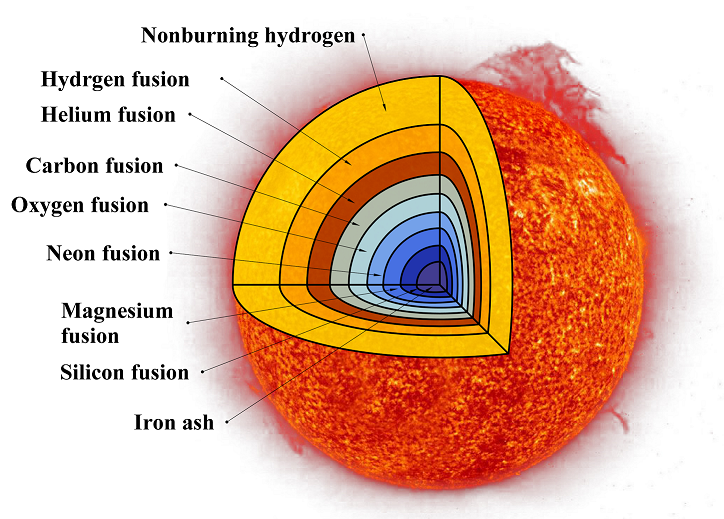
\includegraphics[scale=0.6]{graph/ch1/onion_1}}
    \caption{Onion-like structure just before the end of the life for a massive star.}
    \label{fig:onion}
  \end{center}
\end{figure}

The nuclear reactions are not only the main energy sources that act against the gravitational contraction of stars, but also the only mechanism by which all isotopes  except for hydrogen are synthesized in the universe. The production of energy and elements by nuclear processes, in turn, explains the structure and evolution of the universe. Stellar nucleosynthesis is therefore a  critical topic that focuses on how elements are produced in the universe and its influence on star evolution. For the understanding of the past and the present, as well as to make predictions for the development of the universe, it is, therefore, essential to fully understand the synthesis of the elements in our universe.


\section{The $s$-process components}

As mentioned in the last section,  nuclei heavier than iron (A $\textgreater$ 56) are mainly synthesized by processes involving the neutron capture (i.e. the neutral-particles capture) on preformed seed nuclei instead of charged particle reactions. This is due to the fact that the temperature required to produce enough energy for charged particle reactions to overcome the rapidly rising Coulomb barriers of the heavy nuclides would be so high that they would destroy those seed nuclei through photonuclear reactions\citep{Boyd}.%[R. Boyd]


\begin{figure}[tpb]
  \begin{center}
    \centerline{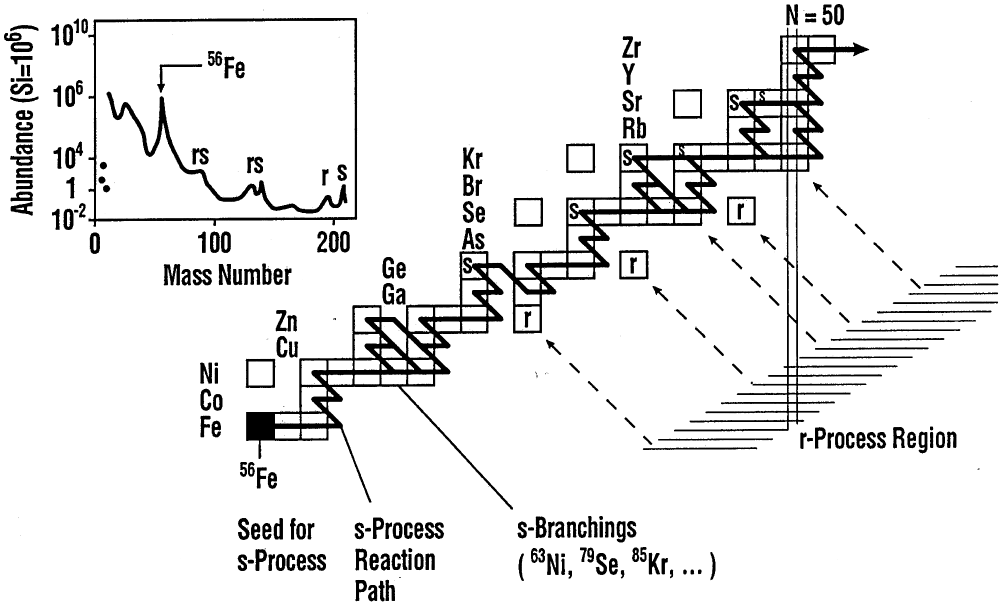
\includegraphics[scale=0.5]{graph/ch1/n-cap}}
    \caption{Chart of the nuclides showing the path of the s-process starting from  iron~\citep{Kappeler2011}. See retails in the text.}
    \label{fig:n-cap}
  \end{center}
\end{figure}

The s-process proceeds through nuclei that $\beta$-decay rapidly compared with the time between successive neutron capture.  It starts from the iron seed along the group of stable nuclei and will eventually terminate at the most massive stable nucleus $^{209}$Bi. Fig.~\ref{fig:n-cap} illustrated the path of the s-process in a portion of the chart of the nuclides, along with the r-process which  drives the nuclei to the neutron-rich region. 
The inset gives the solar abundance distribution relative to 10$^6$ Si atoms. The sharp abundance peaks denoted as $s$  near the mass numbers A = 88, 138 and 208 (corresponding to the neutron magic numbers of N = 50, 82 and 126, respectively) are due to the s-process,  indicating  the impact of the nuclear structure effect.
The s-process can be considered as a ��secondary�� process
in the sense that the seed nuclei (typically $^{56}$Fe) must have existed at the stellar birth as the stellar evolution does not produce the heavy elements before those burning phases are triggered. This is in contrast to  the r-process which generally is referred to as a `primary' process as it is likely to proceed on freshly produced seeds in the interiors of extreme stellar environment (Type-II supernovae for instance).


%%%%%


According to the classical approach to describe s-process model\citep{Kappeler1989}\citep{CLAYTON1961}, under neutron irradiation, for an  isotope A the change in abundance ($N_s(A)$) with time  can be written as
 \begin{equation}
    \label{Na_rate}
    \begin{aligned}
        dN_s(A)/dt = \lambda_n(A-1)N_s(A-1) - (\lambda_n(A) + \lambda_{\beta}(A)) N_s(A)
    \end{aligned}
\end{equation}
where the neutron capture rate $\lambda_n$ is proportional to the neutron capture cross section $\sigma$ and the neutron flux $\Phi$ by $\lambda_n = \sigma \Phi$. The neutron flux $\Phi$ is the product of neutron density $n_n$ and the thermal neutron velocity $v_T = (2kT/m)^{1/2}$, where $m$ refers to the reduced mass. The $\beta$-decay rate $\lambda_\beta=\ln 2/t_{1/2}$ for a radioactive isotope A.

With two assumptions in the classical model: (i)The s-process temperature $T$ is constant as the neutron capture rates are almost independent of  temperature and (ii) The radioactive nuclei on the synthesis path is stable ($\lambda_\beta \ll \lambda_n$), Eq~\ref{Na_rate} can be rewritten by the time-integrated neutron flux $\tau = \int \Phi dt$,
 \begin{equation}
    \label{Na_rate2}
    \begin{aligned}
        dN_s(A)/d\tau = \sigma(A-1)N_s(A-1)-\sigma(A)N_s(A)
    \end{aligned}
\end{equation}
When the system reaches the equilibrium, the production and destruction terms in Eq.\ref{Na_rate2} leading to a constant product of cross section and s-process abundance, written as $\sigma N_s$. $\sigma N_s$ is the characteristic quantity of the classical s-process.

As the abundances of s-only isotopes cannot only be reproduced by a single irradiation of an iron seed\citep{CLAYTON1961}, the assumption that the neutron exposure was in the form of   an exponential distribution\citep{SeegerP1965}, written as
 \begin{equation}
    \label{rho}
    \begin{aligned}
        \rho(\tau) = \frac{f N_{56}}{\tau_0} \exp(-\tau/\tau_0),
    \end{aligned}
\end{equation}
where $\rho$ represents the fraction of iron seeds that have been irradiated in a unit time. $\tau_0$ refers to the mean neutron exposure,  $N_{56}$ is  the number of irradiated iron seeds and $f$ is the fraction of the number of the iron nuclei.

Eq.\ref{rho}  leads to the  solution of the system of Eq.~\ref{Na_rate2}
 \begin{equation}
    \label{product}
    \begin{aligned}
    \sigma(A)N_s(A) = \frac{f N_{56}}{\tau_0} \prod^A_{i=56}[1+(\sigma(i)\tau_0)^{-1}]^{-1}
    \end{aligned}
\end{equation}

% EXplain the measured data point in Fig.2
As mentioned in the last section, according to the phenomenological s-process model analysis for Eq.~\ref{product}~\citep{Kappeler1989}~\citep{CLAYTON1961}, there are three distinct components are needed to  fit the solar abundance distribution of the s-process elements, which is described by the $N_{s}(A) \langle \sigma_s \rangle $ curve as a function of neutron exposure. Fig.~\ref{fig:abundance} shows the clear separation of the two s-process components, the weak component and the main component, by depicting the cross section times the s-process abundance ($N_{s}(A) \langle \sigma_s \rangle $) as a function of the mass number. The measured data points correspond to the experimental measurement for the s-only nuclei. The thick solid line represents the  main component calculated from the means of the classical model, which fits the measured data well especially for nuclei with large mass numbers. The thin solid line refers to the result of the weak component in  massive stars, which is successful in describing s-process products with mass number up to A = 90.
%One should also notice that at A = 84, 138 and 208 the cross sections for
%neutron captures into new neutron shells are very small since these nuclei correspond
%to magic neutron numbers N = 50, 82 and 126, respectively. Therefore, for a given
%supply of neutrons, the  product drops to a new plateau as shown in Figure\ref{fig:abundance}.

%State that 3 components are needed to fit the data(thin line)


%Introduce those 3 components

\begin{figure}[tpb]
  \begin{center}
    \centerline{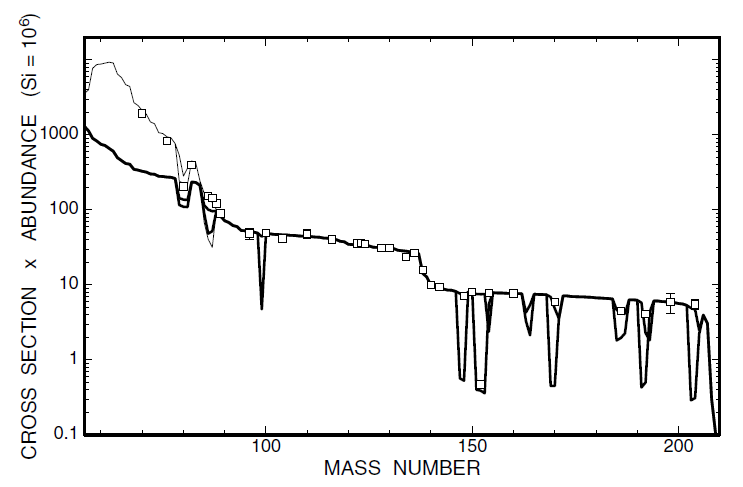
\includegraphics[scale=0.6]{graph/ch1/abundence}}
    \caption{The product of the cross section and the s-process abundance v.s. the mass number. The thin line refers to the weak component in massive stars obtained by means of the classical model and the thick line represents the main component. The  data points denote the experimental results for the s-only nuclei. Figure from Ref.~\citep{Kappeler2011}}
    \label{fig:abundance}
  \end{center}
\end{figure}

%%%%

It is reasonable to assume that different sites are required for each of the observed s-process components. The astrophysics sites for main- and weak- components are described in the following subsections.


\subsection{AGB stars}

The main component of the s-process is shown to occur in low mass as well as intermediate mass (0.8M$_\odot$ $\lesssim$ M $\lesssim$ 8M$_\odot$ ) Asymptotic Giant Branch (AGB) stars during a thermal pulsing phase, accounting for the s-process nuclei in the mass range  90 $\lesssim$ A $\lesssim$ 208.  The model of an AGB star can be explained by the evolution of M = 5$M_{\odot}$ in  the Hertzsprung-Russel (HR) diagram, which plots the luminosity versus surface temperature of a star (shown in Fig.~\ref{fig:AGB}).

Core hydrogen burning sets in on the zero age main sequence (ZAMS) and   slowly continues,  converting hydrogen in its core into helium. Once a significant fraction of about 10$\%$ of central hydrogen is exhausted, which takes about 10$^9$ to 10$^{10}$ years, the star will move towards the red giant phase as the envelope expands. Between the first dredge-up and the red giant branch (RGB), the hydrogen shell burns  and brings helium to the core, increasing the temperature rapidly, therefore, the core helium burning is ignited. The envelope expands once again as the core burns its helium until the core helium runs of out of materials. At this point the hydrogen and helium shell will burn periodically around the C-O core. The star will then undergo a thermal pulsing (TP) AGB phase, where the helium shell surrounding the C-O core and the hydrogen in the outer convective shell  burn alternately. At this moment the star appears close to the RGB, giving the name of AGB phase.


\begin{figure}[tpb]
  \begin{center}
    \centerline{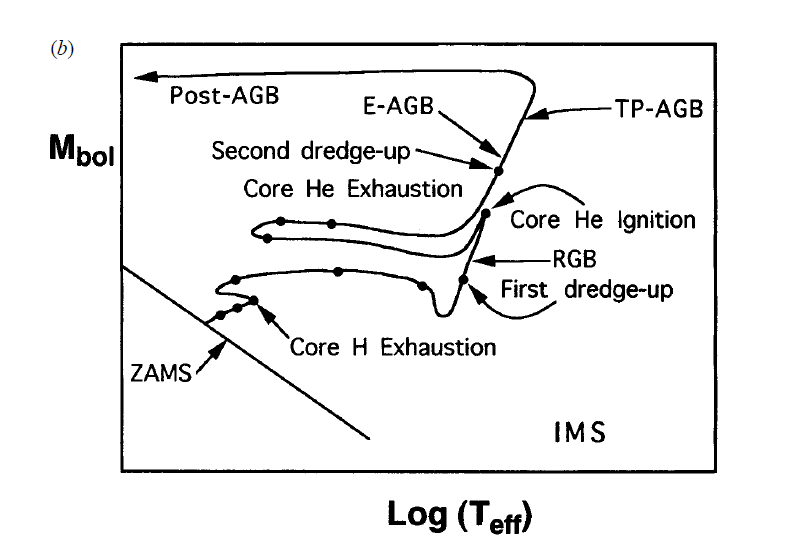
\includegraphics[scale=0.6]{graph/ch1/AGB_HR}}
    \caption{HR diagram for a AGB star (M = 5 M$_\odot$).}
    \label{fig:AGB}
  \end{center}
\end{figure}

During the AGB phase, after the quiescent of a TP, the convective envelope penetrates below the hydrogen shell and the helium shell, mixing the carbon and oxygen into the intershell, and adds a small amount of protons into the top layer of the helium from the hydrogen shell. The protons then can be captured by $^{12}$C through the reaction $^{12}$C(p,$\gamma$)$^{13}$N($\beta^+v$)$^{13}$C, producing a so-called $^{13}$C pocket. The $^{13}$C is consumed in the helium intershell in the AGB phase before a new TP develops. This is the dominant neutron source for the main s-process component.

\subsection{Massive stars}

Another s-process site, the weak $s$-process component is thought to originate mainly from the core helium burning stage in massive stars (M $\gtrsim$ 13M$_\odot$) during the pre-supernovae evolution, producing light s-elements in the A $\sim$ 60 - 90 mass range.

At the beginning of the helium burning in the core, the $^{14}$N produced by the preceding CNO cycles during the hydrogen burning phase are rapidly converted to $^{22}$Ne by successive $\alpha$ captures and a $\beta$-decay through  $^{14}$N($\alpha$,$\gamma$)$^{18}$F($\beta ^{+} v$) $^{18}$O($\alpha,\gamma$)$^{22}$Ne. Towards the end of the helium burning when most of the helium is exhausted (about 10$\%$ left), when the temperature reaches $\sim$ 2.5 GK, the $^{22}$Ne($\alpha$,n)$^{25}$Mg neutron source becomes operative. The remaining $^{22}$Ne left over from helium burning is the main neutron source during the subsequent carbon shell burning. This process is sensitive to the treatment of mixing at the edge of the convective zone during the end of the core helium burning.


%The main neutron source triggering the s-process in massive stars is the 22Ne(a,n) reaction.




\section{Astrophysical Importance of the $^{25}$Mg(d,p)$^{26}$Mg}


So far it is known that $^{22}$Ne($\alpha$,n)$^{25}$Mg is the main neutron source for the  weak s-process component in massive stars during core helium burning and in AGB stars during helium-shell burning. Most of the neutrons are captured by various neutron poisons, especially by $^{25}$Mg since it has a very large neutron capture cross sections, therefore dramatically reducing the number of neutrons per $^{56}$Fe seed. The competing reaction  $^{22}$Ne($\alpha$,$\gamma$)$^{26}$Mg is another neutron poison, since the cross sections of both reactions are  dominated by the contribution of low energy and natural parity resonances\citep{Kappeler2011}. Considerable effort has been made in the past to measure the low energy resonances in $^{22}$Ne($\alpha$, $\gamma$) and $^{22}$Ne($\alpha$, n) \citep{Wolke1989}\citep{Jaeger2001}to determine their impact on the channel branching and the overall efficiency of the neutron sources in the stellar environment. There are a number of low energy resonances which have not yet been measured because of the extremely small cross sections. Only limited experimental information is available about these states in the compound nucleus $^{26}$Mg which primarily results from transfer reactions, neutron capture or photo-excitation studies. This lack of information introduces considerable uncertainties into the calculation of the reaction rates and can have an significant influence on the calculated nucleosynthesis in massive stars.


The lowest-lying known resonance in the $^{22}$Ne + $\alpha$  channel has been observed at a center of mass energy of E$\alpha$ = 703 keV corresponding to an excitation energy in $^{26}$Mg of 11.318 MeV \citep{Wolke1989}\citep{Jaeger2001}. Additional 38 states have been reported between the alpha threshold at 10.615 MeV and this resonance, which might contribute to the stellar-reaction rate. 16 of these states are above the neutron threshold of E$\alpha$ = 478 keV (E$x$ =11.093 MeV) and can contribute to both the ($\alpha$,n)- and the ($\alpha$, $\gamma$)-reaction channel. The actual number of relevant states will be lower because only natural parity states can be populated in the  $^{22}$Ne + $\alpha$ system.

Since the ($\alpha$,n) and the ($\alpha$, $\gamma$) reaction are competing with each other, it is necessary to know the ratio of the  gamma to neutron width, $\Gamma_{\gamma}/\Gamma_{n}$.
The role of the $^{22}$Ne($\alpha$,n) reaction as a stellar neutron source might be impacted if the stellar-reaction rate for $^{22}$Ne($\alpha$, $\gamma$) reaches a few percent of the $^{22}$Ne($\alpha$,n) reaction. Detailed information is available about neutron-unbound states within the first 500 keV above the neutron threshold from (n,$\gamma$) experiments~\citep{Massimi}~\citep{Koehler2002}. These two experiments provide precise excitation energies and determine the $\gamma$ and neutron widths for these states with ratios $\Gamma_{\gamma}/\Gamma_{n}$ ranging from 10$^{-4}$ to 10. However they failed to observe the 703 keV resonance which has been observed in both reactions. In addition, the (n,$\gamma$) experiments mainly populate s- and p-wave resonances and definite spin and parity assignments were not possible for a majority of the observed states.

To clarify the situation we propose a high resolution measurement of the $^{25}$Mg(d,p)$^{26}$Mg
reaction to populate states within 1 MeV above the alpha threshold using the Grand Raiden Spectrometer at the Research Center for Nuclear
Physics (RCNP) in Osaka, Japan. The goals of  the experiment are (i) Precise measurement of excitation energies; (ii) Restricting spin and parity of observed states; (iii) Observation of the 11.32 MeV state which is missing in the n-ToF measurement; (iv) Determination of the neutron spectroscopic factors.

% % uncomment the following lines,
% if using chapter-wise bibliography
%
% \bibliographystyle{ndnatbib}
% \bibliography{example}

%%
% Modified by Megan Patnott
% Last Change: Jan 18, 2013
%
%%%%%%%%%%%%%%%%%%%%%%%%%%%%%%%%%%%%%%%%%%%%%%%%%%%%%%%%%%%%%%%%%%%%%%%%
%
% Modified by Sameer Vijay
% Last Change: Wed Jul 27 2005 13:00 CEST
%
%%%%%%%%%%%%%%%%%%%%%%%%%%%%%%%%%%%%%%%%%%%%%%%%%%%%%%%%%%%%%%%%%%%%%%%%
%
% Sample Notre Dame Thesis/Dissertation
% Using Donald Peterson's ndthesis classfile
%
% Written by Jeff Squyres and Don Peterson
%
% Provided by the Information Technology Committee of
%   the Graduate Student Union
%   http://www.gsu.nd.edu/
%
% Nothing in this document is serious except the format.  :-)
%
% If you have any suggestions, comments, questions, please send e-mail
% to: ndthesis@gsu.nd.edu
%
%%%%%%%%%%%%%%%%%%%%%%%%%%%%%%%%%%%%%%%%%%%%%%%%%%%%%%%%%%%%%%%%%%%%%%%%

%
% Chapter 2
%

\chapter{Gnu Things are Good Things for all Graduate Students or so it Seems}
\label{chap:golfing}

\section{Gnu See, Gnu Do, Gnu Goes Golfing with Green Golf Genes and
  Gesticulates Grapes}

So why do gnus do what they do?  This is a perennial question that has
yet to be answered definitively by scientists.  Is their future
somehow tied inexplicably with that of humans?  Hard to say, but we do
feed them a lot.  It has even been theorized that rotundness is a
symbol of status or class within the Gnus; those who are more
productive (i.e., cute, furry, friendly) will be fed more than those
who are less so.  So the more rotund, the higher status one has in the
Gnu society.

One could extrapolate this to mean that there is a super-Gnu out there
somewhere; the biggest, rotundest Gnu that you've ever seen, probably
of epic proportions!  This would have to be the Leader of Gnus, or LoG
for short.  But the LoG would definitely have to be the cutest,
furriest, and most friendly Gnu that you've ever seen.

\subsection{The LoG}

So how does the LoG get chosen?  Ultimately by humans.  So we can say
that the Gnu society is perhaps the truest democracy that has ever
existed; the leader is chosen by merit, and chosen by complete
outsiders.  As such, the LoG must truly epitomize all that Gnus stand
for: opposedness to overmanagement, cuteness, friendliness, and
furriness~\citep{gloonson98:_gnuly_discov_gnus}.  The gnus themselves
vote at an anual election, based upon these attributes (campagaining
is an anethema to Gnus; see Section~\ref{sec:groovin-gnus}).

\subsubsection{Election Data}
\label{sec:data}

Table~\ref{tbl:votes} shows the latest electoral college voting by the
LoG for the year 2000.  Each Gnu is scored on a scale of one to ten on
the attributes described above.  The results shown in the table are
average scores in each category for all votes; the Gnu's final score
is shown in the final column.

%
% Be aware that page-spanning tables a Very Odd Creatures.  The
% "longtable" environment in LaTeX does some deep Voodoo to make
% everything work out properly.  One of its deep incantations is to
% make the table appear as though it is double spaced.  You can fix
% this by trailing each line with "\\[-6em]" instead of just "\\".
% When using longtable it is also important to compile your file
% more than once. But you're probably already doing this to get
% the internal references correct, anyway.
%

\begin{center}
  \begin{longtable}{lccccc}
    \caption{Electoral College Results for the \NoCaseChange{LoG} Election in the Year
2000\label{tbl:votes}\/}\\
        \toprule
        Candidate\footnote{note all names begin with G} & Anti-management & Cuteness & Friendliness & Furriness & Aggregate \\
        \midrule
\endfirsthead % Everything above goes at the top of the 1st page only
% As with the first header, we don't want obscene amounts of space for
% subsequent headings either, and eliminate an em of whitespace.
  \caption[]{{\em Continued}}\\
  \midrule
  Candidate & Anti-management & Cuteness & Friendliness & Furriness & Aggregate \\
  \midrule
\endhead % Everything above here (and below the \endfirsthead) goes at the top
         % of continuation pages.  The [] argument prevents a duplicate
         % entry from appearing in the table of contents.
% The following 3 lines are provided as an example only -- per ND
% guidelines, the footer at the bottom of a page for a longtable
% should not have a bottom line.  Only the absolute bottom of the
% table should have a final \bottomline

%  \midline
%  \multicolumn{6}{|r|}{\textit{continued}\ldots} \\
%  \bottomrule
\endfoot % The above section goes at the bottom of continuation pages
  \bottomrule
\endlastfoot % The very last bottom of the table
    Glen & 6.2 & 7.0 & 6.1 & 9.8 & 7.2 \\
    Goober & 6.9 & 2.1 & 5.7 & 4.1 & 4.6 \\
    Genevra & 2.2 & 2.0 & 1.1 & 1.1 & 1.6 \\
    Greg & 8.3 & 0.4 & 1.1 & 9.5 & 4.8 \\
    Gina & 6.0 & 7.8 & 6.4 & 4.9 & 6.2 \\
    Geof & 1.1 & 8.7 & 3.7 & 7.3 & 5.2 \\
    Grendel & 2.8 & 1.7 & 3.4 & 3.2 & 2.7 \\
    Geronimo & 1.2 & 1.2 & 8.8 & 2.2 & 3.3 \\
    Gabrielle & 4.7 & 3.6 & 0.8 & 2.0 & 2.7 \\
    Giovani & 8.4 & 5.8 & 3.4 & 7.4 & 6.2 \\
    Graham & 4.7 & 5.8 & 5.3 & 0 & 3.9 \\
    Gil & 5.9 & 4.0 & 5.5 & 7.6 & 5.7 \\
    Gerald & 2.0 & 3.7 & 8.0 & 4.3 & 4.5 \\
    Guilani & 7.7 & 3.9 & 2.7 & 6.4 & 5.1 \\
    Guido & 7.6 & 4.3 & 6.5 & 1.0 & 4.8 \\
    Godzilla & 5.1 & 2.2 & 5.3 & 6.9 & 4.8 \\
    Gail & 5.7 & 7.9 & 4.1 & 1.0 & 4.6 \\
    Garth & 4.7 & 7.1 & 2.5 & 3.0 & 4.3 \\
    Gavin & 1.1 & 9.5 & 0.4 & 8.0 & 4.7 \\
    George & 9.5 & 4.5 & 9.1 & 7.5 & 7.6 \\
    Gunnar & 1.4 & 5.8 & 4.8 & 6.2 & 4.5 \\
    Gillian & 7.6 & 9.0 & 6.4 & 4.6 & 6.9 \\
    Greta & 1.5 & 0.5 & 0.9 & 7.7 & 2.6 \\
    Gabby & 1.2 & 3.3 & 7.0 & 2.1 & 3.4 \\
    Gaetena & 6.8 & 1.9 & 4.1 & 8.3 & 5.2 \\
    Ganet & 2.3 & 1.1 & 8.5 & 7.3 & 4.8 \\
    Gardenia & 1.8 & 9.5 & 9.9 & 3.0 & 6.0 \\
    Genna & 5.2 & 3.7 & 3.4 & 3.8 & 4.0 \\
    Genesis & 1.7 & 8.3 & 6.7 & 4.9 & 5.4 \\
    Genaveve & 4.7 & 8.9 & 3.4 & 9.2 & 6.5 \\
    Gene & 3.3 & 6.9 & 0.6 & 5.5 & 4.0 \\
    Gilda & 5.2 & 4.6 & 9.9 & 1.4 & 5.2 \\
    Goldie & 8.9 & 9.1 & 2.0 & 8.2 & 7.0 \\
    Grace & 5.9 & 3.2 & 3.1 & 4.3 & 4.1 \\
    Gretchen & 4.5 & 6.5 & 1.6 & 1.3 & 3.4 \\
    Garrick & 4.8 & 5.7 & 9.4 & 5.1 & 6.2 \\
    Gallagher & 7.4 & 0.4 & 7.6 & 0.4 & 3.9 \\
    Gerry & 1.4 & 8.8 & 4.7 & 0.5 & 3.8 \\
    Gertrude & 9.1 & 8.3 & 0.4 & 5.5 & 5.8 \\
    Gehosephet & 6.6 & 2.9 & 8.3 & 4.4 & 5.5 \\
    Gohn & 8.7 & 2.6 & 7.4 & 2.3 & 5.2 \\
    Gibby & 8.7 & 6.9 & 4.7 & 7.2 & 6.9 \\
  \end{longtable}
\end{center}

As you can see from Table~\ref{tbl:votes}, George (my favorite Gnu)
won for the year 2000, with an aggregate score of 7.6.

% % uncomment the following lines,
% if using chapter-wise bibliography
%
% \bibliographystyle{ndnatbib}
% \bibliography{example}

%
\chapter{EXPERIMENTAL SETUP AND PROCEDURES}

\section{Experiment Overview}
We measured the $^{25}$Mg(d,p)$^{26}$Mg reaction  at the Research Center for Nuclear Physics (RCNP) of the Osaka University using the AVF Cyclotron, the WS course and Grand Raiden (GR) spectrometer. The layout of the facility is shown in Figure.\ref{fig:RCNP_layout}. The deuteron beam was accelerated to 56 MeV by the  K = 140 MeV Azimuthally Varying Field (AVF) cyclotron and transported to the  GR through the WS beam line. For highest resolution the beam line was dispersion matched to the GR spectrometer.

\begin{figure}[tpb]
  \begin{center}
    \centerline{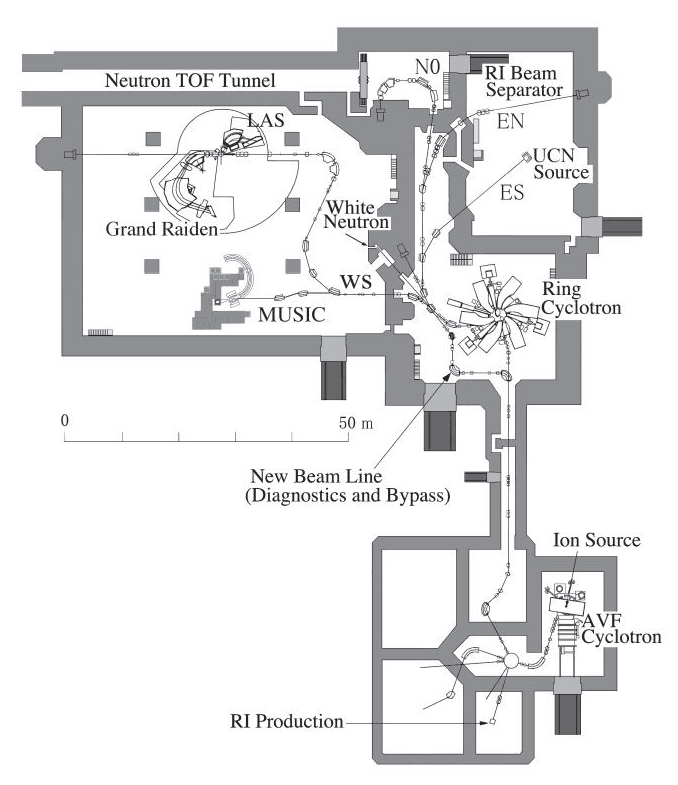
\includegraphics[scale=0.6]{graph/ch3/RCNP_layout}}
    \caption{Floor plan of the experimental facility at RCNP. The Ring Cyclotron was bypassed in this experiment.~\citep{Hatanaka2013}
    }
    \label{fig:RCNP_layout}
  \end{center}
\end{figure}
   % 

A self-supporting $^{25}$Mg target (enrichment $\approx$ 97.8$\%$) with a thickness of 1 mg/cm$^2$ was placed at the center of the scattering chamber. The total energy resolution of approximately 20 keV was  achieved, resulting from 10 keV energy loss and 4.5 keV of energy straggling of the scattering protons, as well as 1 keV of target inhomogeneity and 2.5 keV from the GR resolving power of 37000. In addition, a $^{24}$Mg target with the thickness of 1.2 mg/cm$^2$ and Mylar foils [(C$_{10}$H$_8$O$_4$)$_n$] of 6$\mu$m/(29 mm $\times$ 29 mm) were used for background measurements of reactions on carbon and oxygen.

%%%%%%
The GR spectrometer was originally placed at 0$^\circ$. The full acceptance was 20 mrad in the horizontal direction and 40 mrad in the vertical direction. The deuteron beam was dumped into the Faraday Cup inside the first dipole (D1) magnet, which is shown in Fig \ref{fig:GR_FC}. This Faraday Cup was also used for monitoring the beam current. For scattering angles in the range of $2^\circ \textendash 6 ^\circ$ the Faraday cup Q1-FC downstream of the quadrupole Q1 was used. For larger angles, the Faraday cup in the scattering chamber was employed.
In order to achieve best possible spatial and angular resolution, full dispersion matching\citep{Wakasa200279} including the over-focus mode \citep{FUJITA200217} were applied. Outgoing protons were momentum analyzed and focused at the focal plane where the focal plane detector system was placed. The focal plane detector system consisted of two multi-wire drift chambers (MWDCs)  and two plastic scintillators. Particles were then traced back with  the MWDCs allowing the reconstruction of particle trajectory. The protons were identified with the scintillators by the timing and energy loss differences. The scintillators also produced  the start and stop triggers for the MWDCs.


%Protons scattered by the target placed in the target chamber were analyzed by the GR %spectrometer and detected by the Focal Plane Detectors at the end of the beam line.



\section{The Grand Raiden Spectrometer}
The Grand Raiden (GR) spectrometer was designed for high resolution measurements. It consists of three dipoles (D1, D2 and DSR) magnets, two quadrupole  (Q1 and Q2) magnets, a sextupole  (SX)  magnet and a multipole  (MP) magnet (See Fig.~\ref{fig:GR_layout}). The design parameters of the specification and ion-optical properties are listed in Table.~\ref{tb:GR}. Its large magnetic rigidity of B$\rho=$5.4 T$\cdot$m  and high resolving power of $p/\Delta p=\dfrac{D_x}{M_x \Delta x_0}=37000$ (where $\Delta x_0$ = 1 mm for a monochromatic beam spot size, $M_x$ and $D_x$ refer to the magnification and the dispersion of the spectrometer, respectively) make it stand out for high resolution measurement.
The Q1 magnet is placed close to the scattering chamber in order to achieve large vertical angle acceptance.
The second-order ion-optical aberrations are in part minimized by the SX magnet. The MP magnet generating the quadrupole, sextupole, octupole and decapole is installed between the D1 and D2 magnet to further correct higher-order aberrations. The DSR magnet is an auxiliary magnet for measuring the spin-rotation parameters and was not used in the present experiment. The GR spectrometer is designed in such way that particles with different magnet rigidities are transported to different horizontal positions in the focal plane.

\begin{figure}[tpb]
  \begin{center}
    \centerline{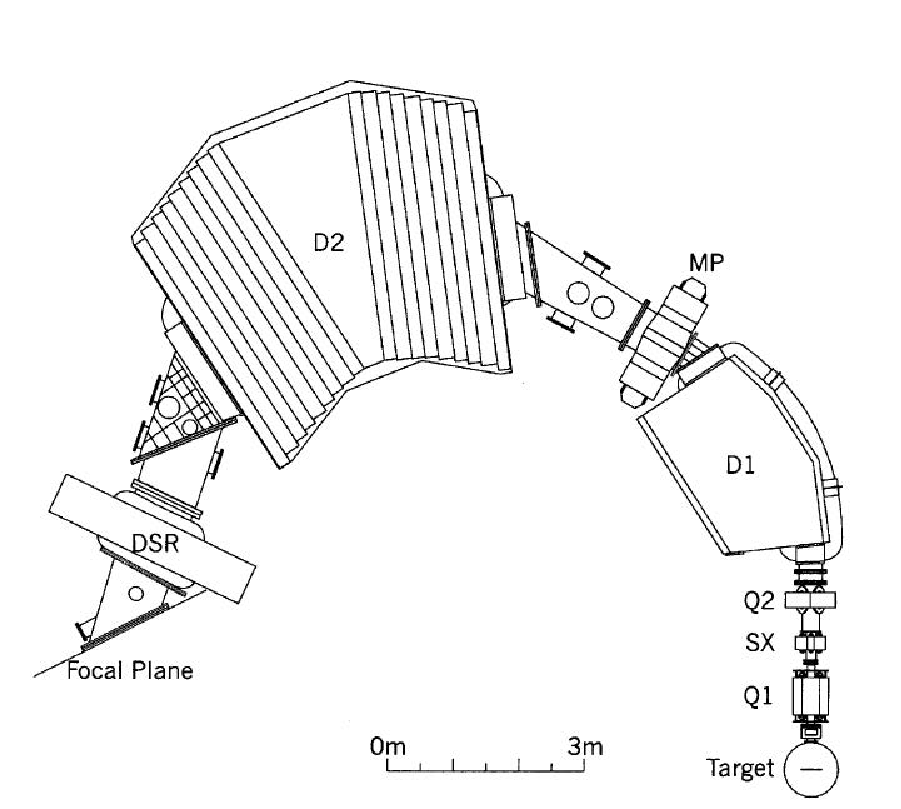
\includegraphics[scale=0.7]{graph/ch3/GR_layout}}
    \caption{The schematic layout of the Grand Raiden (GR) Spectrometer. ~\citep{Wakasa200279} }
    \label{fig:GR_layout}
  \end{center}
\end{figure}


\begin{table}[tpb]
  \setlength{\capwidth}{0.7\textwidth}
  \begin{center}
    \caption{DESIGN VALUES FOR THE GRAND RAIDEN SPECTROMETER ~\citep{Fujiwara1999484} }
    \label{tb:GR}
    \begin{tabular}{lr} \toprule
      \hline
      Mean orbit radius                         &           3 m \\
      Total deflection angle                    &           162$^{\circ}$\\
      Angular range                             &           0$^{\circ}$ to 90$^{\circ}$\\
      Focal plan length                         &           150 cm\\
      Tilting angle of focal plane              &           45.0$^{\circ}$\\
      Maximum field strength of dipoles (D$_1$, D$_2$)    &       1.8 T\\
      Vertical magnification (M$_y$)            &           5.98\\
      Horizontal magnification (M$_x$)          &           -0.417\\
      Momentum dispersion (D$_x$)               &           15.45 m\\
      Momentum range                            &           5\%\\
      Momentum resolution (p/$\Delta$p)         &           37000\\
      Horizontal acceptance angle               &           $\pm$ 20 mrad\\
      Vertical acceptance angle                 &           $\pm$ 40 mrad\\
      Solid angle                               &           3.2 msr \\\bottomrule
    \end{tabular}
  \end{center}
\end{table}



\section{Dispersion Matching}
The high resolving power of the  spectrometer gives an optimum energy resolution of about 2.5 keV for  56 MeV deuterons  for a monochromatic image size on target of $\Delta  x = 1$ mm ($\Delta K=(1.70\cdot \Delta p/p)K = 2.5$ keV). However, the momentum spread of the incident beam produced by the cyclotron usually makes the spectral resolution worse in the achromatic beam transportation. To achieve the high resolution measurement, the dispersion of the beam line and the dispersion of a spectrometer has to be  matched.
The dispersion matching method can be explained by using matrices for ion optics in the TRANSPORT notations in the phase space. A particle in the system can be described by coordinates $\boldsymbol{x}=(x, \theta, \delta)$, where the $x$, $\theta$ and $\delta$ are the horizontal displacement, angle and fraction of the momentum deviation defined by $p/\Delta p$ respectively,  and they are defined as differences from the central trajectory.
Assume particles pass through the exit point of the accelerator with the coordinates $\boldsymbol{x_0}=(x_0, \theta_0, \delta_0)$ and end up with the coordinates $\boldsymbol{x_1} =(x_1, \theta_1, \delta_1)$ at the target position after transport through the beam line system  described by the matrix $\textbf{B}=\{b_{\mu \nu}\}$, where the matrix elements represent $x$, $\theta$, $\delta$ with 1, 2 and 6, respectively. $\delta_0=\delta_1$, $b_{61}=b_{62}=0$ and $b_{66}=1$ as the energy does not change in the magnetic field.
Particles are then scattered in the target position with $\boldsymbol{x_2}=(x_2, \theta_2, \delta_2)$ by the target matrix $\textbf{T}$ and reach the focal plane with $\boldsymbol{x}=(x, \theta, \delta)$ transported by the spectrometer matrix $\textbf{S}=\{s_{\mu \nu}\}$. By combining $\textbf{B}$, $\textbf{T}$ and $\textbf{S}$, the transformations at the focal plane position are given by
\begin{equation}
    \label{eq:x_fp}
    \begin{aligned}
     x_{fp} & =  x_0(s_{11} b_{11} T + s_{12} b_{12})               \\
            & + \theta_0(s_{11} b_{12} T + s_{12} b_{22})          \\
            & + \delta_0(s_{11} b_{16} T + s_{12} b_{26} + s_{16} C)  \\
            & + \Theta(s_{12} + s_{16} K)                           \\
    \end{aligned}
\end{equation}
\begin{equation}
    \label{eq:theta_fp}
    \begin{aligned}
     \theta_{fp} &= x_0(s_{21} b_{11} T + s_{22} b_{21})        \\
                 &+ \theta_0(s_{21}b_{12}T + s_{22} b_{22})     \\
                 &+ \delta_0(s_{21}b_{16}T + s_{22}b_{26} + s_{26}C) \\
                 &+ \Theta(s_{22} + s_{26}K)                    \\
    \end{aligned}
\end{equation}
where $T$, $C$, $K$ are the target function, the dispersion-matching factor and  kinematic factor,  respectively,  and defined as
\begin{equation}
    \label{eq:TKC}
    \begin{aligned}
     T & = \frac{\cos(\alpha - \phi_T)}{\cos \phi_T}                        \\
     C & = \frac{p_{in}}{p_{out}} \cdot \frac{\partial p_{out}}{\partial p_{in}} \\
     K & = \frac{1}{p_{out}} \cdot   \frac{\partial p_{out}}{\partial \alpha}  \\
    \end{aligned}
\end{equation}

\begin{figure}[tpb]
  \begin{center}
    \centerline{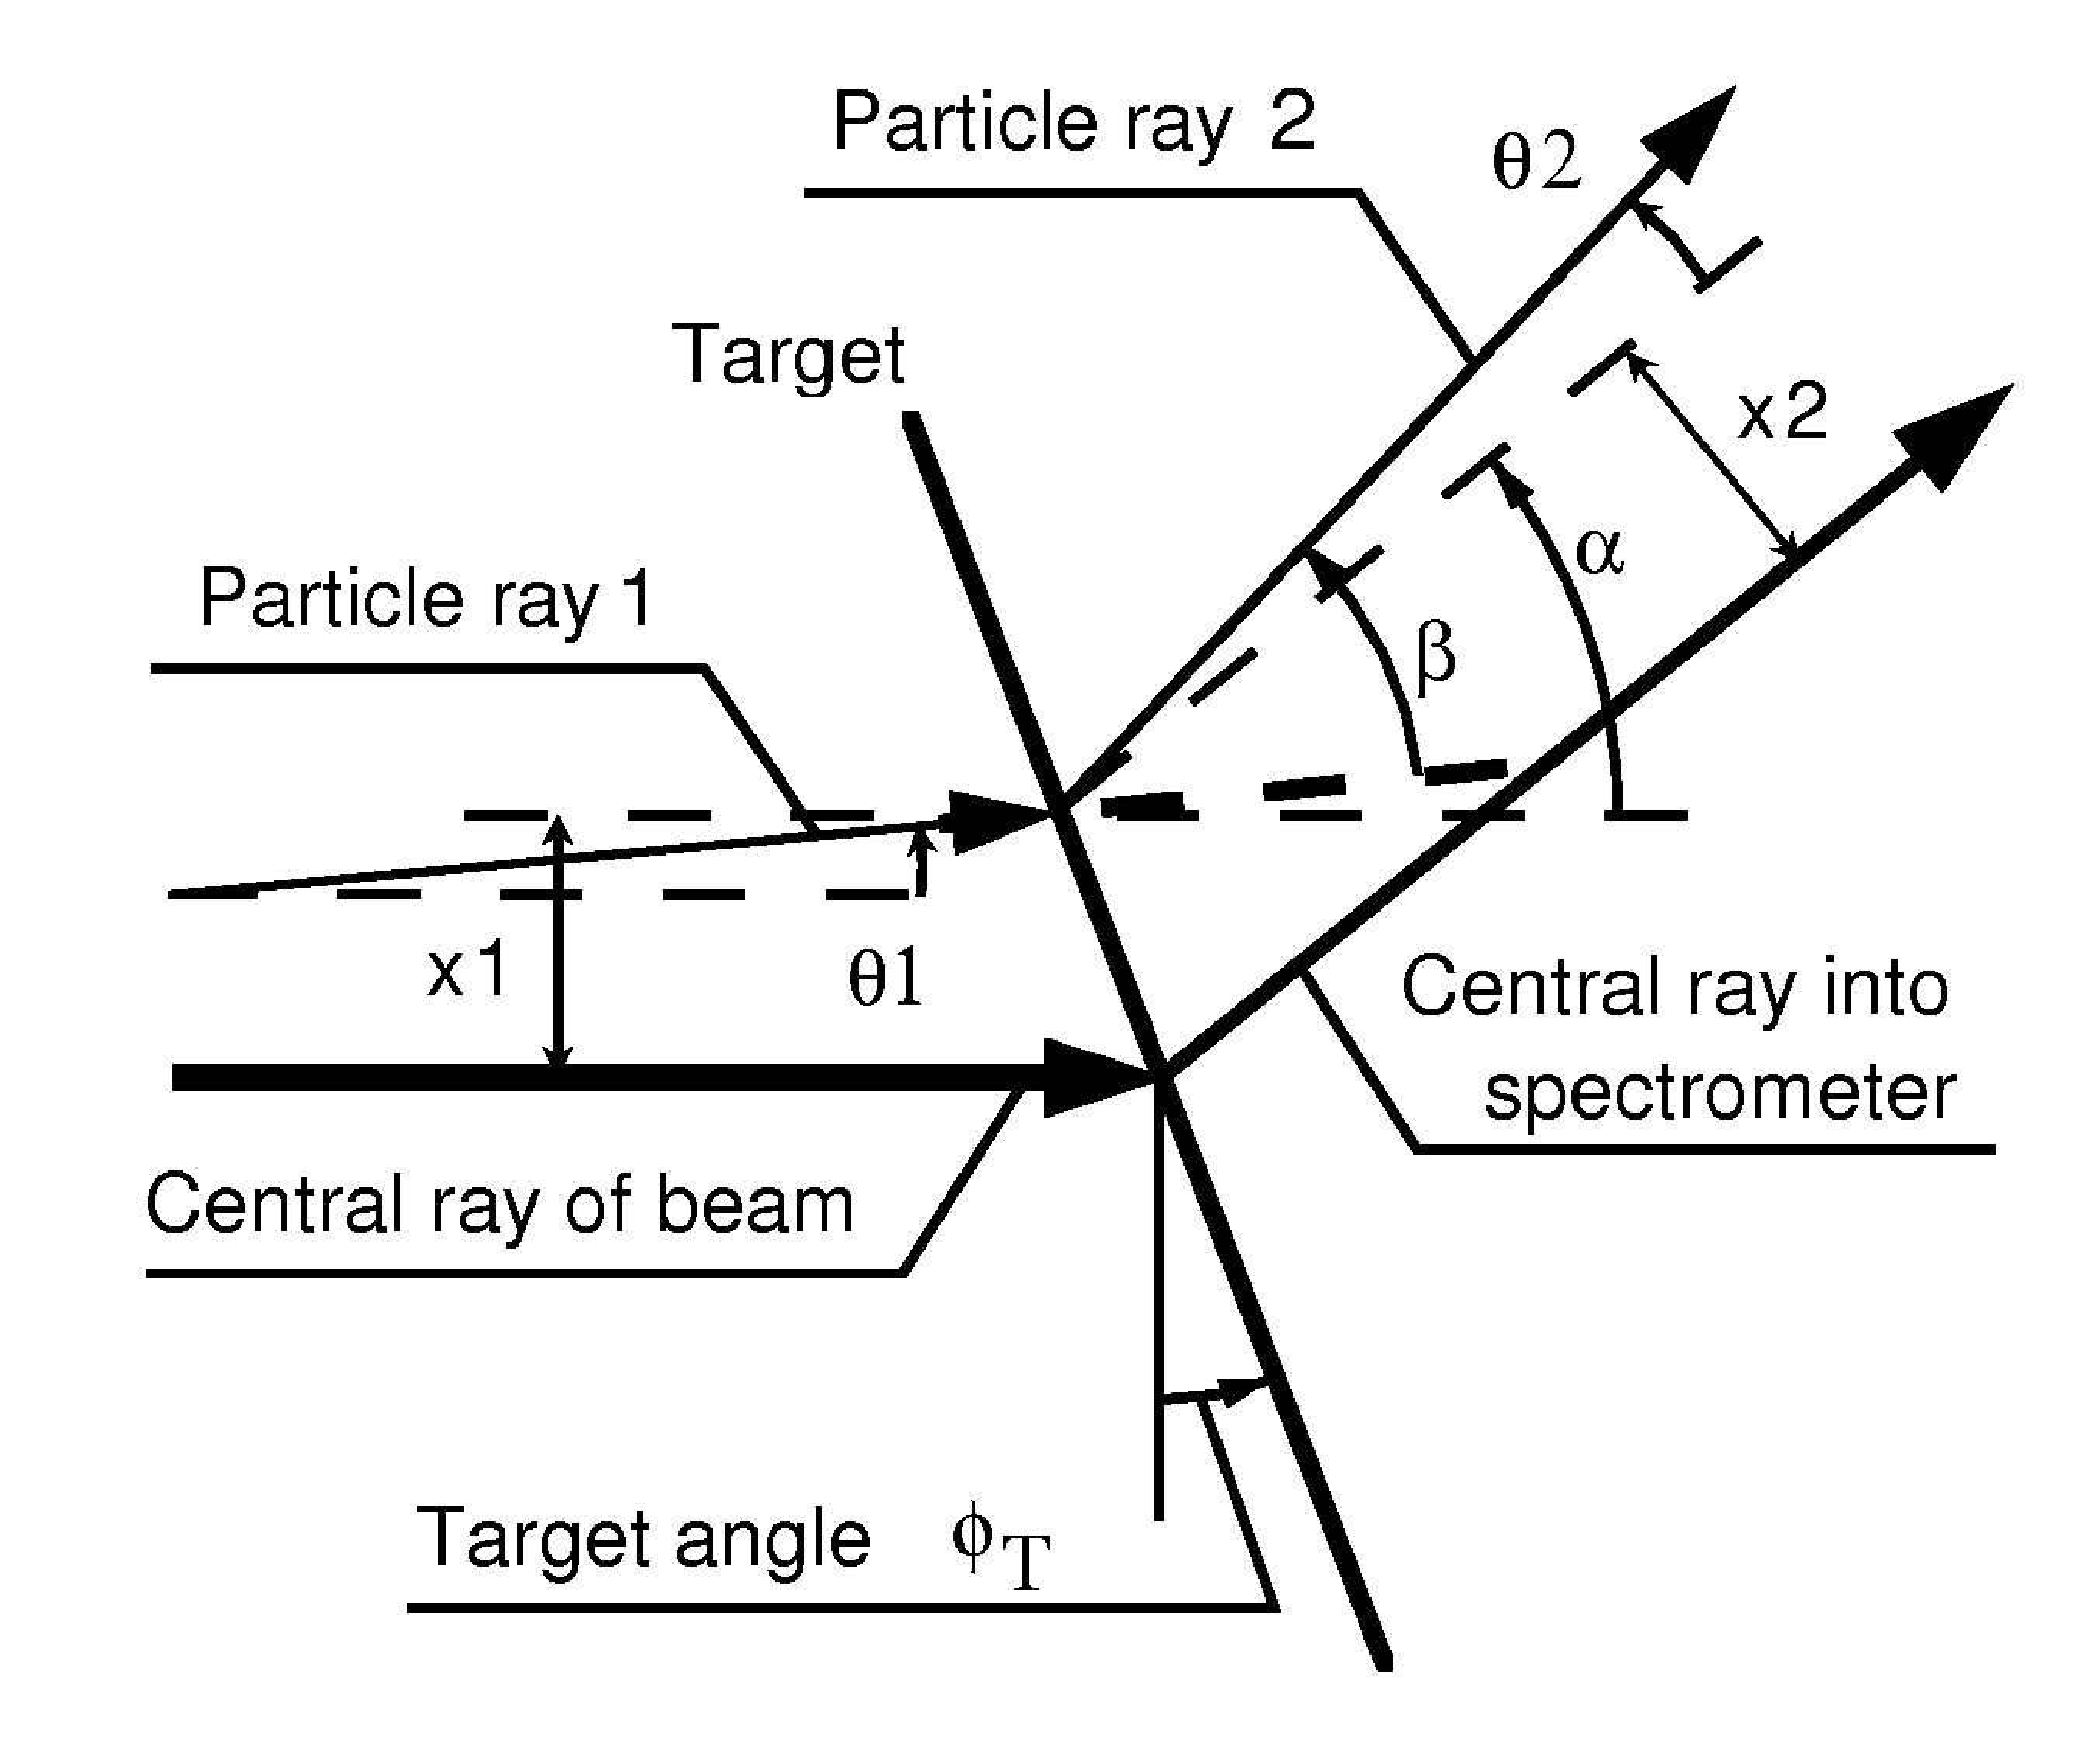
\includegraphics[scale=0.18]{graph/ch3/kinectics}}
    \caption{Schematic representation of the scattering of one particle with coordinates ($x_1$, $\theta_1$ )
relative to the central ray of the beam. The ($x_2$, $\theta_2$) are coordinates of outgoing particles and $\alpha$ is the
scattering angle of the central ray.}
    \label{fig:kinectics}
  \end{center}
\end{figure}

In the target function $T$, $\alpha$ is the reaction angle in the laboratory frame and $\phi_T$ is the tilting angle of the target. In the dispersion-matching factor $C$, $p_{out}$ is the momentum of the outgoing particle at the target and $p_{in}$ is the momentum of the incident particle at the target position. There are several special cases can simplify the calculation. For instance, for an elastic scattering, $C=1$ and at 0$^\circ$, the kinematic factor $K=0$.
The geometry of the kinematics is illustrated in Fig. ~\ref{fig:kinectics}, where $\theta_1$ is the angle between the incident particle  and the central ray of the beam and $\theta_2$ is the angle between the outgoing particle and the central ray into the spectrometer. The true scattering angle is thus given by
\begin{equation}
    \label{eq:beta}
    \begin{aligned}
    \beta=\alpha+(\theta_2-\theta_1)
    \end{aligned}
\end{equation}
The momentum at the focal plane is then given as
\begin{equation}
    \label{eq:sigma_fp}
    \begin{aligned}
    \delta_{fp} = \theta_2 = K \Theta + C\delta_0
    \end{aligned}
\end{equation}
where $\Theta=\theta_1-\theta_2$ is the relative scattering angle.


The best possible spectral resolution can be achieved by minimizing the image size of $x_{fp}$ as well as realizing the angular dispersion matching. As a result, the coefficients of  $\theta_0$, $\sigma_0$ and $\Theta$ in  Eq.~\ref{eq:x_fp}  should be eliminated and the coefficient of $\delta_0$ in Eq.~\ref{eq:theta_fp} should be minimized. The $\delta_0$ dependence of $\theta_{fp}$ in Eq.~\ref{eq:theta_fp} is large since a large dispersion $b_{16}$ of the beam line is required for the lateral dispersion matching.

The minimization of the coefficient of $\Theta$ in Eq.~\ref{eq:x_fp} gives
 \begin{equation}
    \label{eq:s12}
    \begin{aligned}
        s_{12} = -s_{16}K
    \end{aligned}
\end{equation}
which is called the kinematic correction.

The minimization of the $\theta_0$ dependence in Eq.~\ref{eq:x_fp} results in
 \begin{equation}
    \label{eq:b_12}
    \begin{aligned}
        b12=-\frac{s_{12}}{s_{11}}\frac{b_{22}}{T}
    \end{aligned}
\end{equation}
which is known as the focusing matching.

To realized the so-called the dispersion matching, by minimizing the coefficients in  $\sigma_0$ in  Eq.~\ref{eq:x_fp} both lateral dispersion matching and angular dispersion matching can be  achieved by setting the matrix elements of the beam line as:
 \begin{equation}
    \label{eq:b16}
    \begin{aligned}
        b_{16} = -\frac{s_{16}}{s_{11}}(1 + s_{11}s_{26}K - s_{21}s_{16}K)\frac{C}{T}
    \end{aligned}
\end{equation}
and
 \begin{equation}
    \label{eq:b26}
    \begin{aligned}
        b_{26} = (s_{21}s_{16} - s_{11}s_{26})C
    \end{aligned}
\end{equation}
Here the relationship $s_{11}s_{22}-s_{12}s_{21}=1$ is used to make the expression simpler. The matching conditions given by Eq.~\ref{eq:b16} and Eq.~\ref{eq:b26} are the so-called the lateral dispersion matching and the angular dispersion matching, respectively.

The resolving power of the matched system is given by
 \begin{equation}
    \label{eq:R}
    \begin{aligned}
        R=(1/2x_0)(s_{16}/M_{ov})
    \end{aligned}
\end{equation}
where $M_{ov}=(s_{11}b_{11}T+s_{12}b_{12})$ refers to as an overall magnification and has the form
 \begin{equation}
    \label{eq:M}
    \begin{aligned}
        M=(s_{11}b_{11}T-s_{16}b_{12}K)
    \end{aligned}
\end{equation}
if the matching conditions are satisfied.


The concept of dispersion matching conditions is shown in Fig.~\ref{fig:dispersion}. Only trajectories of central rays scattered at 0$^{\circ}$ are shown in these figures. In the left panel (a), three trajectories with different momenta $\sigma_0=0$, $\pm\Delta p/p$ are shown for a beam with the achromatic focus at the target position ($b_{16}=b_{26}=0$). Particles with different $\delta_0$ are dispersed by the spectrometer and the resolution focused in the focal plane are limited by the beam momentum spread.
The middle panel (b) shows beam trajectories when the lateral dispersion-matching is realized ($b_{16}$ matched, $b_{26}=0$).
Particles with different momenta $\delta_0$ are focused at different lateral positions on the target and this dispersion is compensated by the dispersion of the spectrometer. In such way the spectral resolution is no longer limited by the momentum spread of the beam.
However, under this condition, rays with different $\delta_0$ may cross the focal plane with different angles $\theta_{fp}$, which gives rise to an ambiguity in determining the scattering angles at the target. This can be eliminated when both lateral and angular dispersion-matching have been realized simultaneously, which is shown in the right panel (c). By adjusting the dispersion of the positions and incident angles for beam rays appropriately, the positions and angles of particles measured at the focal plane ($x_{fp}$, $\theta_{fp}$) do not depend on the beam dispersion at the target and the measured angle in the focal plane corresponds to a unique scattering angle.




\begin{figure}[tpb]
  \begin{center}
    \centerline{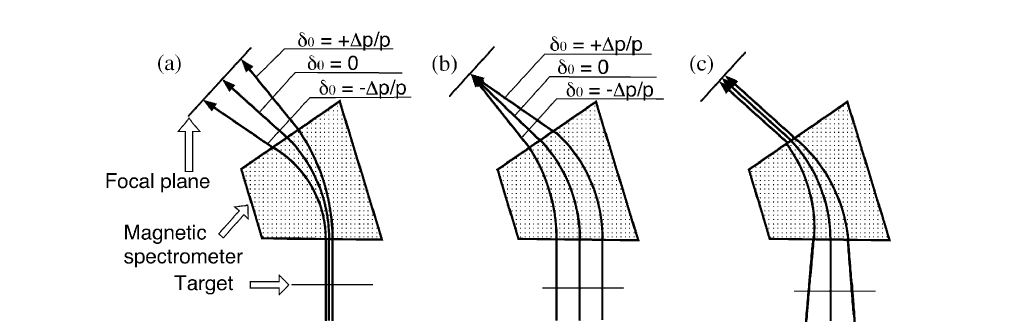
\includegraphics[scale=0.7]{graph/ch3/dispersion}}
    \caption{Schematic ion trajectories under different matching conditions of a beam line and a magnetic spectrometer.(a)When achromatic mode is achieved; (b)when lateral dispersion matching is realized; (c)when both lateral and angular dispersion matching are realized. The rays with the different momenta are shown.~\citep{FUJITA200217}}
    \label{fig:dispersion}
  \end{center}
\end{figure}


\section{0$^{\circ}$ Measurement and the Over-focus Mode}
In order to determine the angular distribution, an angular measurement is needed with a good resolution. Near and including 0$^{\circ}$, high resolution measurements of both horizontal and vertical angle components  are equally important such that the scattering angle can be precisely determined. However, since GR spectrometer is a horizontal-bending high-resolution spectrometer, the vertical angle magnification is small ($\approx$ 0.17)  so that the vertical focusing quadrupole magnet is placed as close to the target as possible in order to realize a large vertical acceptance.
Under this condition, it is impossible to achieve a vertical resolution at the target better than 12 mrad. Therefore, the vertical angle resolution cannot be determined as good as the horizontal angle resolution in the normal point-to-point focus mode.

In order to improve the vertical angular resolution, the ion-optical mode called off-focus mode has been developed at RCNP.  The ion-optical properties of the spectrometer in the vertical direction were considered in the transfer matrix up to the second order:
 \begin{equation}
    \label{eq:y_fp}
    \begin{aligned}
        y_{fp} &= (y|y)y_{tgt}+(y|\phi)\phi_{tgt} + (y|yx)y_{tgt}x_{tgt} \\
               &+ (y|\theta)y_{tgt}\theta_{tgt} + (y|y\delta)y_{tgt}\delta \\
               &+ (y|\phi x)\phi_{tgt} x_{tgt} + (y|\phi \theta) \phi_{tgt} \theta_{tgt} \\
               &+ (y|\phi \theta) \phi_{tgt} \delta           \\
               &+higher \ order \ terms
    \end{aligned}
\end{equation}
where $y_{tgt}$ and $\phi_{tgt}$ are the vertical position and the outgoing angle of a particle at the target and $x_{tgt}$ and $\theta_{tgt}$ are the horizontal position and angle, respectively. $(y|y)$, $(y|\phi)$ etc. are matrix elements of the spectrometer  that transports coordinates from the target to the focal plane coordinates.  $\delta$ is the fractional momentum spread of the incoming beam at the target.


In Fig.~\ref{fig:off_focus} the vertical trajectories for three different focus modes are depicted. In the normal focus mode of GR spectrometer shown in the top panel (a), the term $(y|\phi)$  from Eq.~\ref{eq:y_fp} is set to  zero for the central ray (R = 300 cm). By increasing the strength of the Q1 magnet of GR spectrometer such that $(y|\phi)>0$, particles with different vertical outgoing angles from the target, $\phi_{tgt}$, will be transported to different vertical positions $y_{fp}$ in the focal plane. This mode is called over-focus mode and the vertical trajectories are shown in the middle panel (b). Similarly, the bottom panel (c) shows trajectories of the transport in the under-focus mode where the strength of the Q1 magnet is decreased and $(y|\phi)<0$. Therefore, it is possible to determine  $\phi_{tgt}$ values from the measured value of $y_{fp}$ in the off-focus modes.
\begin{figure}[tpb]
  \begin{center}
    \centerline{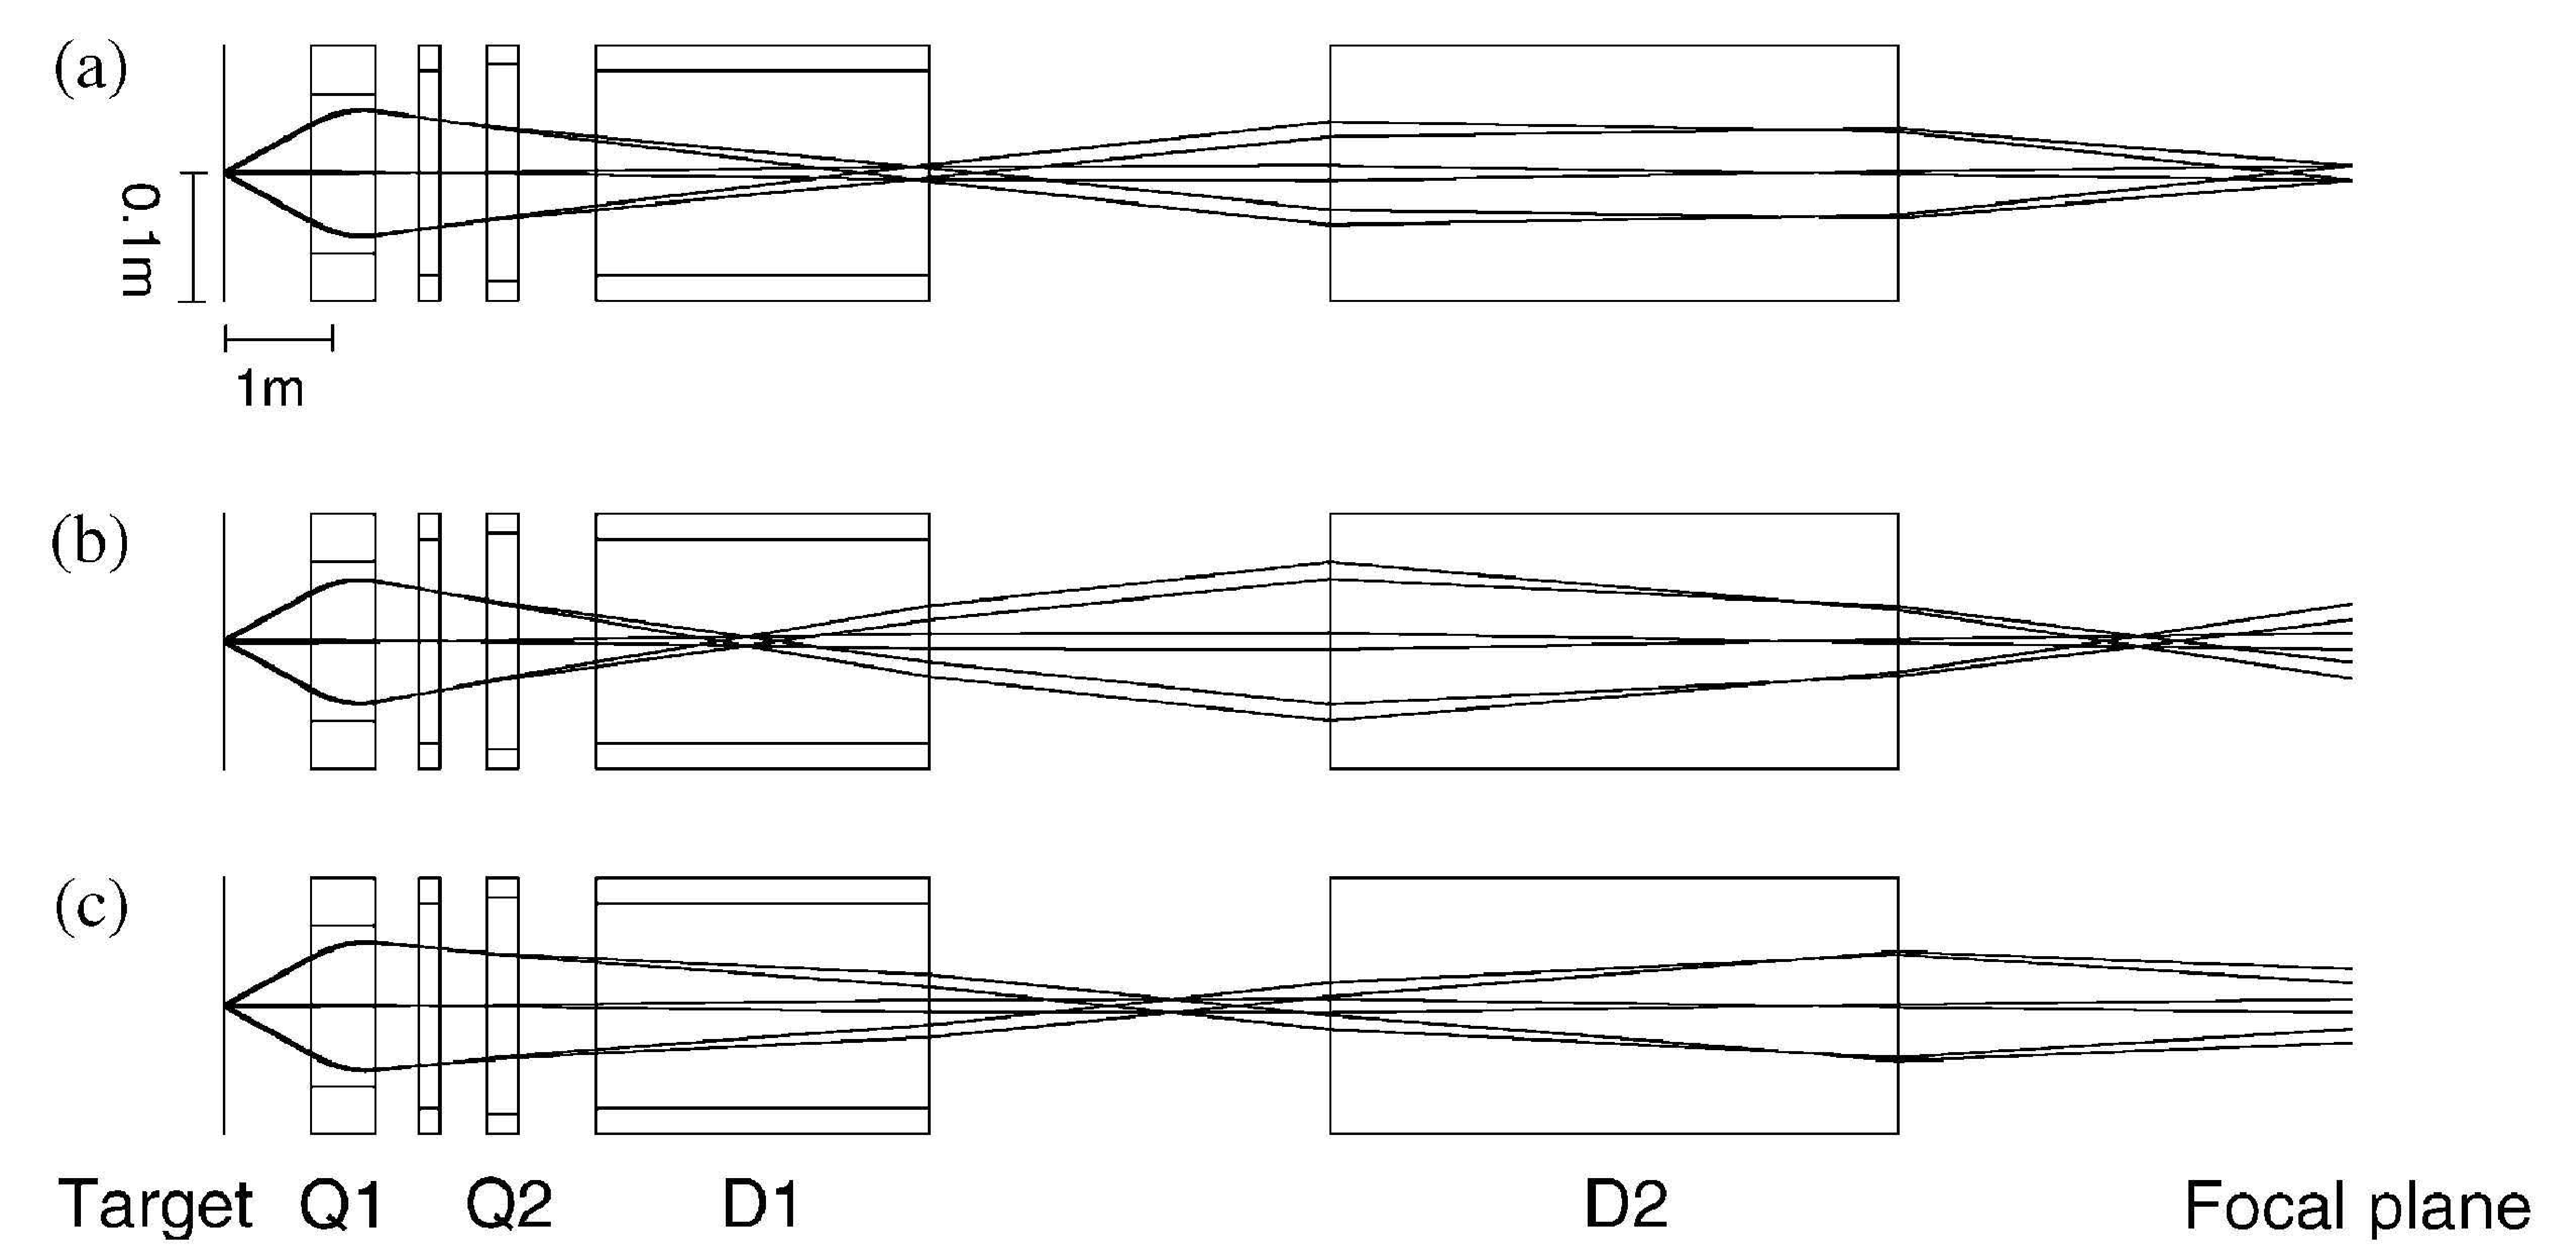
\includegraphics[scale=0.15]{graph/ch3/focus_mode}}
    \caption{Envelope of analyzed particles in Grand Raiden for vertical position with $\phi_{tgt}=0$, $\pm$46 mrad and $y_{tgt}=\pm$1. (a) Normal focus mode. (b) Over focus mode. (c) Under focus mode.~\citep{FUJITA200155}}
    \label{fig:off_focus}
  \end{center}
\end{figure}
In order to calibrate vertical components of scattering angle $\phi_{tgt}$ in the off-focus mode accurately, the ambiguities from the angle determination should be small. The largest ambiguity comes from the vertical beam spot size  $\Delta y_{tgt}$ due to the large  vertical magnification $(y|y)$ of about 6. Typically, $\Delta y_{tgt}$ is $0.5\textendash 1$ mm, so the $(y|y)\Delta y_{tgt}$ term can bring about $3\textendash6$ mm uncertainty in the vertical focal plane. Such effect can be minimized by  increasing the absolute value of the $(y|\phi)$ term which is adjusted by the strength of the quadrupole magnet Q1.

The experiment was performed in the over-focus mode by increasing the Q1 strength by 8\% as compared with the  normal point-to-point focus. In order to  reconstruct the coordinates at the target position from the measured coordinates at the focal plane, a multi-hole aperture (sieve-slit) was used for the angle calibration.


\section{Focal Plane Detectors}
In the focal plane of the GR spectrometer, two 2-dimensional multi-wire drift chambers (MWDCs) were used in order to measure the positions and angles of the outgoing particles. A set of 3 mm and 10 mm thick $\Delta$E plastic scintillator detectors followed by MWDCs was used to provide energy loss and timing information for particle identification. To increase the energy loss in the plastic sintillators, an aluminum degrader (10 mm thick) was placed between the MWDCs and the plastic sintillators. The layout of the focal plane detector system is illustrated in  Fig.~\ref{fig:PSs}. Under this setting the protons produced by the (d,p) reaction are stopped before they reach the last  plastic scintillator.

\begin{figure}[tpb]
  \begin{center}
    \centerline{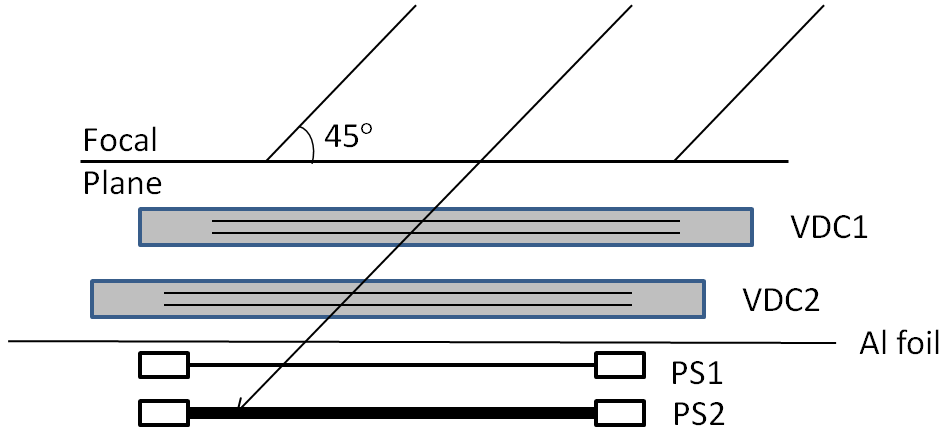
\includegraphics[scale=0.6]{graph/ch3/PSs_new}}
    \caption{Schematic layout of the focal plane detector system. PS1 is 3mm and PS2 is 10mm. An Al degrader is placed in front of the PS1.}
    \label{fig:PSs}
  \end{center}
\end{figure}

The MWDC is also known as the vertical drift chamber (VDC) as  ionized electrons drift perpendicularly to the anode plane. The specifications of the MWDC are listed in Table.~\ref{tb:MWDC}. Each 2-dimensional MWDC consists of two anode-wire planes (X and U) sandwiched between three cathode planes. Anode planes consist of sense wires and potential wires as is depicted in  Fig.~\ref{fig:MWDCs}. The spacing of sense wires is 6 mm for the X-plane and 4 mm for the U-plane, respectively. The potential wires are designed in such way to produce uniform electric field between the cathode plane and the anode plane, supplying the high voltage of -350 V and -500 V in the X-plane and U-plane, respectively. Thus electrons generated by charged particles during the ionization of the detector gas can only produce avalanche near the sense wires. A charged particle trajectory are determined by  measuring the drift-time  of the electrons from four wires, as shown in Fig.~\ref{fig:MWDCs}. For a proper trajectory determination, at least three wire events are  needed to for the drift time measurement per plane. The gas used in the MWDC is a mixture of argon (71.4\%), iso-butane (28.6\%) and iso-propyl-alcohol. The iso-propyl-alcohol was mixed into argon gas with vapor pressure ar 2$^{\circ}$ in order to reduce the deterioration of the gas due to  the aging effect like the polymerization of the gas on the wire surface\citep{Adachi_thesis}\citep{yosoi_thesis}.

\begin{table}[tpb]
  \setlength{\capwidth}{0.7\textwidth}
  \begin{center}
    \caption{SPECIFICATIONS OF MWDCs FOR THE GRAND RAIDEN SPECTROMETER\citep{yosoi_thesis}.}
    \label{tb:MWDC}
    \begin{tabular}{ll} \toprule
      \hline
      Wire configuration                        &           X (0$^{\circ}$ from vertical), U(48.2$^{\circ}$ from vertical) \\
      Active area                               &           1150 mm $\times$ 120 mm\\
      Number of sense wires                     &           192 (X), 208 (U)\\
      Cathode-anode gap                         &           10 mm       \\
      Anode-wire spacing                        &           2 mm\\
      Sense-wire spacing                        &           6 mm (X), 4 mm (U)\\
      Sense-wire thickness                      &           20 $\mu$ m gold-plated tungsten\\
      Potential-wire thickness                  &           50 $\mu$ m gold-plated beryllium-copper\\
      Cathode plane                             &           10 $\mu$ m carbon-aramid foil\\
      Gas mixture                               &           Argon (71.4\%), Iso-butane (28.6\%), \\
                                                &           Iso-propyl-alcohol (trace amount)\\
      Entrance and exit windows                 &           12.5 $\mu$ m aramid foil\\
      Distance between MWDCs                    &           250 mm\\
      \bottomrule
    \end{tabular}
  \end{center}
\end{table}

%\begin{figure}[tpb]
 % \begin{center}
 %   \centerline{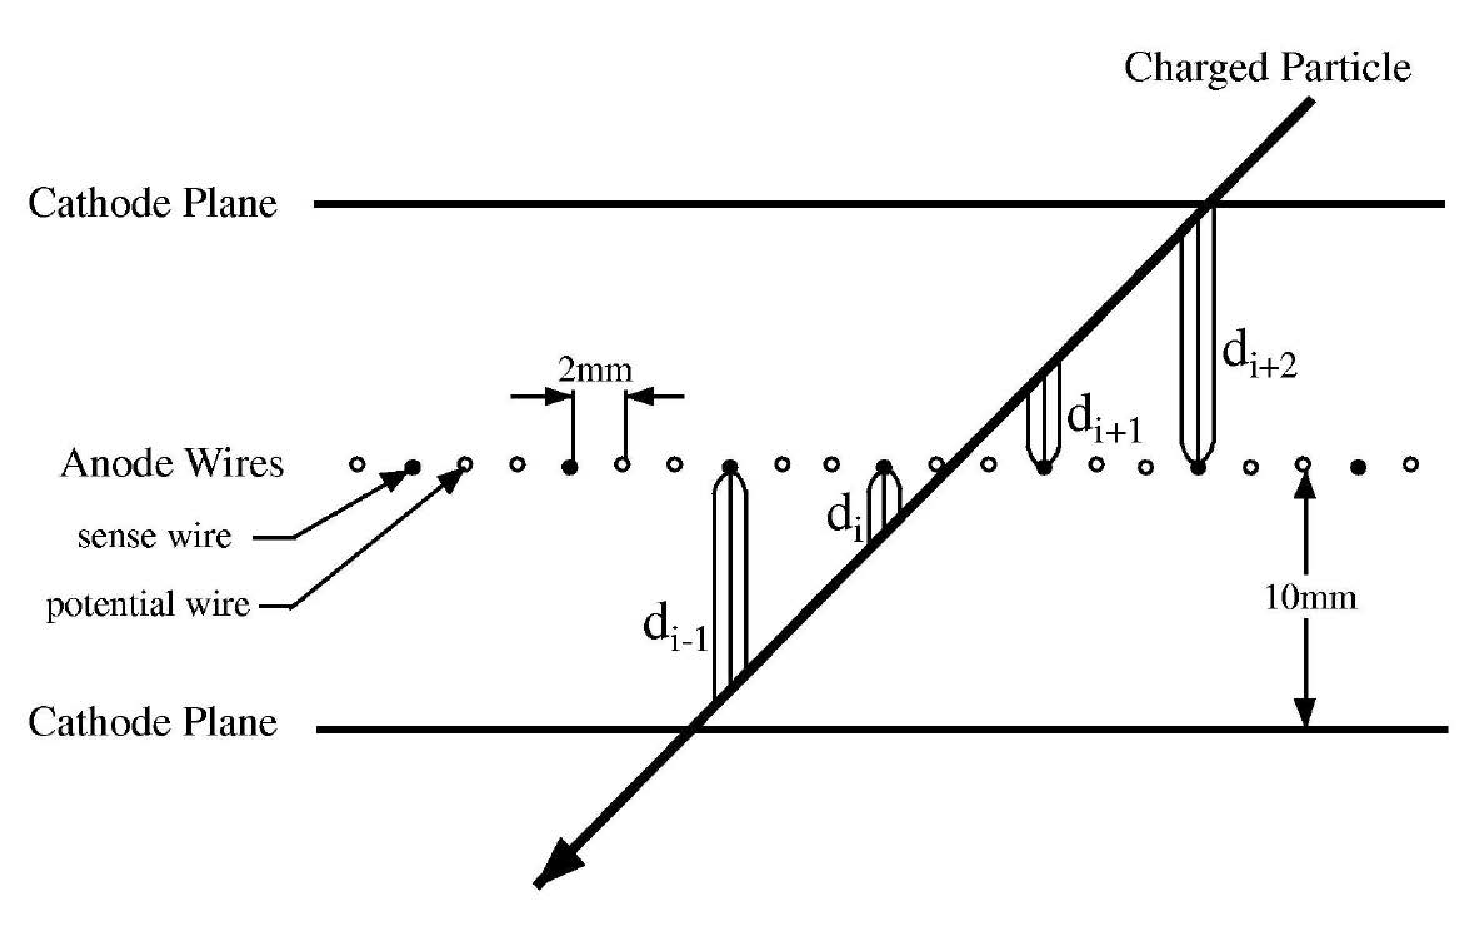
\includegraphics[scale=0.5]{graph/ch3/MWDCs}}
 %   \caption{The schematic structure of an X-plane of the MWDC. A typical track of an charged particle is shown. ~\citep{yosoi_thesis}}
 %   \label{fig:MWDCs.}
 % \end{center}
%\end{figure}

\begin{figure}[tpb]
  \begin{center}
    \centerline{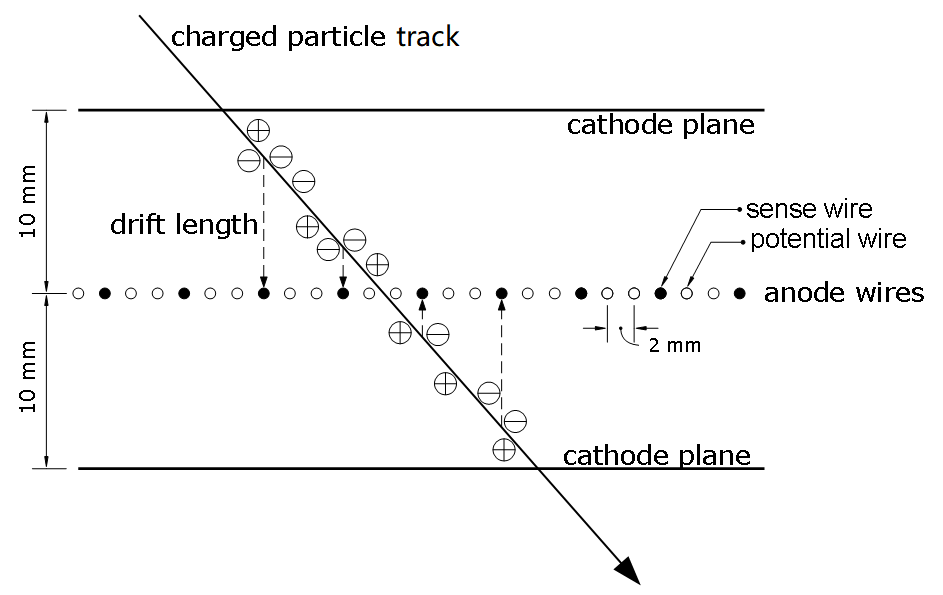
\includegraphics[scale=0.6]{graph/ch4/MWDCs_1}}
    \caption{X-plane configuration of the MWDC. A sample of the charged particle track is shown together with the cathode planes and anode wires.}
    \label{fig:MWDCs}
  \end{center}
\end{figure}

Particles that pass through the MWDCs are detected in two plastic scintillator detectors.
Each scintillator had two photomultipliers (PMs) attached on the left and right side  and were held a voltage of 1800 V and 1450 V for the 3 mm plastic scintillator and 10 mm plastic scintillator, respectively.  The fluorescence is proportional to $\Delta$E of particles, as well as the timing information were produced and collected as events  for particle identification.


\section{Faraday Cup Settings for the (d,p) Reaction}
In addition to the 0$^{\circ}$ data,  measurements were also preformed in the angular range from 5$^{\circ}$ to 40$^{\circ}$ in 5$^{\circ}$ steps. These angular distributions serve several purposes:

1. The measurement of the angular distribution will help to determine the orbital momentum of the transferred neutron.

2. Measurements at different angles allow the identification of lines due to contaminants with different masses owing to their different kinematic shift.

3. Unavoidable light-mass impurities in the target may obscure a peak at one angle but clear this peak at a different angle, allowing its identification.

The Faraday cup setting for 0$^{\circ}$ measurement is shown in Fig.~\ref{fig:GR_FC}. Owing to the differences in magnet rigidities of the deuteron beam and the proton beam from the reaction (ratios in the range of 1.324  to 1.422), the D1 Faraday cup was installed inside the D1 dipole of GR such that deuterons were bent into the Faraday cup while protons were tuned to the focal plane. Since the dispersion in the focal plane is about 15.5m, for a deuteron beam of 56 MeV this allows to measure an excitation range of about 5 MeV and covers the range of interest  about $E_x=$ 9 MeV to 14 MeV with one field setting. At 5$^{\circ}$  the Faraday cup Q1-FC downstream of the quadrupole Q1 was used. For larger angles the Faraday cup inside the scattering chamber was applied.

Nevertheless,  during the experiment there was still a huge deuteron background at 0$^{\circ}$, which was high enough to limit the measurement. This  can be reduced by changing the angle of GR spectrometer to 0.5$^{\circ}$ while still covering the 0$^{\circ}$ measurement. Even though there might still exist  small deuteron background after changing the angle, the remaining background can be removed by using information from the time of flight of the particles.

In this experiment, beam intensities up to 6 nA were used for 0.5$^{\circ}$ and up to 100 nA for higher angle measurements. The live time of the system varied between 93\% and 96\% during the experiment. Three magnet field settings were deployed to cover the whole excitation energy region of interest with sufficient overlap between the different spectra.

The energy calibration was preformed using the $^{25}$Mg(d,p)$^{26}$Mg reaction. The energies of excited states in $^{26}$Mg up to 12 MeV are well known. However, above 7 MeV the level density becomes sufficiently large that it becomes impractical to use these higher-lying states for the calibration. Therefore, protons from lower-lying states were used to calibrate the full focal plane by changing the magnetic settings with sufficient overlap between the different spectra. Three magnetic fields were established in this experiment, which allows us to determine the relatively small but not negligible quadratic term over the full focal plane.  The absolute excitation energy calibration has been  established using the locations of the peaks of the low-lying states in the target nuclei with well-known excitation energies.


\begin{figure}[tpb]
  \begin{center}
    \centerline{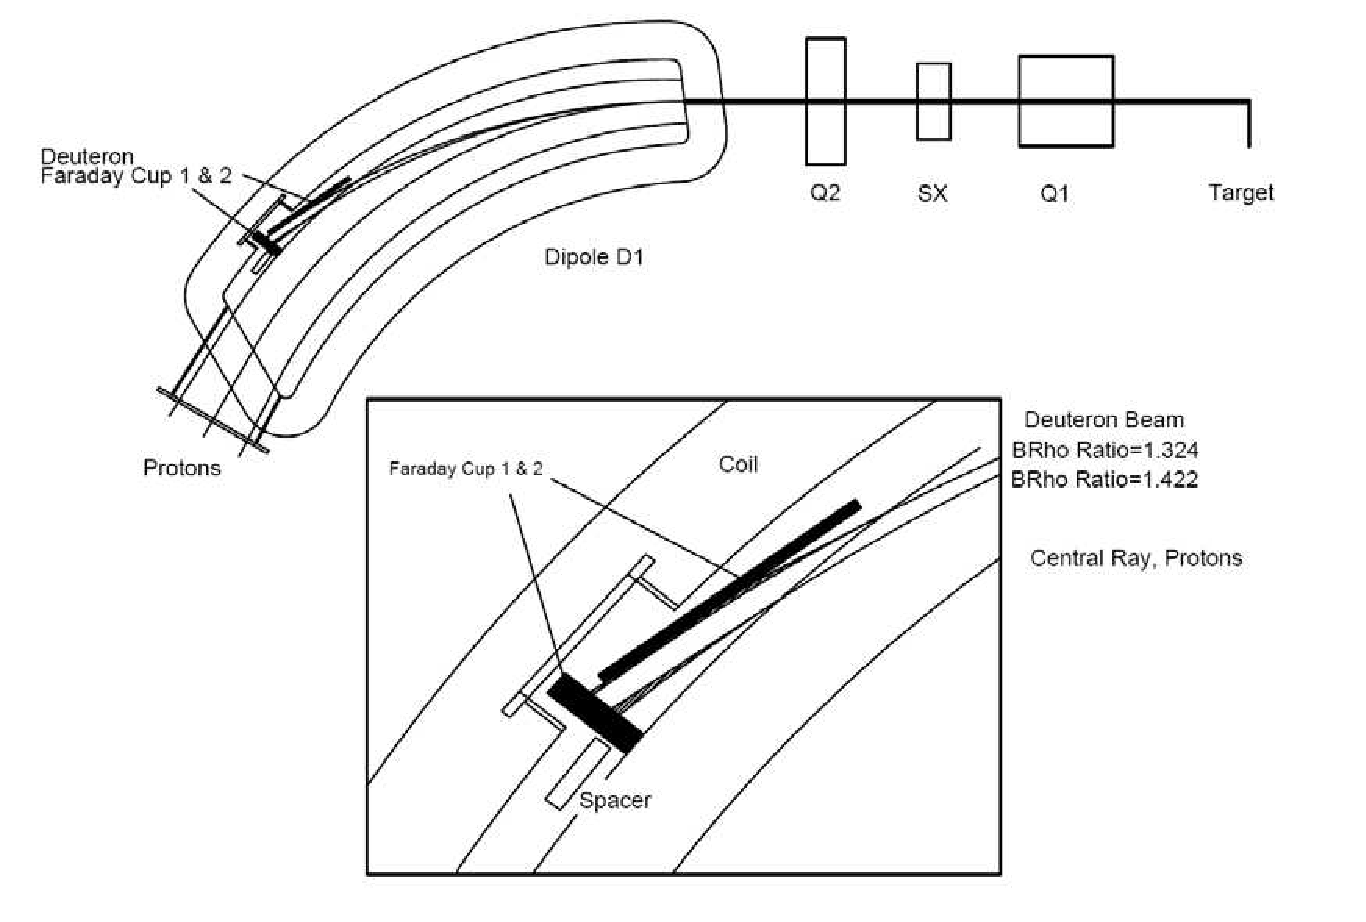
\includegraphics[scale=0.6]{graph/ch3/FC}}
    \caption{The Faraday Cups inside dipole D1 for 0$^\circ$ mode.}
    \label{fig:GR_FC}
  \end{center}
\end{figure}


% % uncomment the following lines,
% if using chapter-wise bibliography
%
 % \bibliographystyle{ndnatbib}
 % \bibliography{reference}

%
%
% Chapter Four


\chapter{RECONSTRUCTION OF THE SPECTRUM}

At RCNP, the raw data  obtained with Grand Raiden was analyzed with  a general purpose analyzer program, Tamii Analyzer, developed by A.Tamii ~\citep{Tamii-ana}.
To extract  clean and optimized spectra with the best possible resolution, events consisting of reaction products of interests without any  unwanted particles, called background, were first selected through the GR spectrometer and were transported to the focal plane. In addition to the particle positions and angles,  data measured by the detectors in the focal plane gave the ToF and energy loss  which were used to further reduce the background.
Finally,  software corrections were applied to correct higher order aberrations to improve the resolution of the spectra. All analyzed results were  stored in the HBOOK file and were plotted using the PAW and ROOT program packages from the CERN library.

\section{Particle Identification and Background Reductions}



In the (d,p) reaction at small scattering angles, most of the particles detected in the focal plane counter were protons - the particles of interests. Any other ``contamination particles'' such as unreacted deuterons and other reaction products had to be prevented from  reaching the focal plane. Neutral particles such as neutrons and $\gamma$-rays produced at the target did not make it to the focal plane through the spectrometer and were not measured by the MWDCs. Therefore, the dominant background particles  measured in this experiment were deuterons. By setting the rigidity acceptance of the spectrometer to the desired proton rigidity, most of the undesirable reaction products including deuterons did not reach the focal plane.
At RCNP, the particle identification for proton events was realized by using time-of-flight (ToF) information and the energy loss difference between the PS1 and PS2 of the GR spectrometer.


The ToF was measured as the time difference between the timing trigger from the plastic scintillator PS1 and the RF signal from the AVF cyclotron. In order to reject deuterons effectively, the corrected  ToF (denoted as RF signals in the analyzer) spectrum was used to be independent of $x_{fp}$ and $\theta_{fp}$, defined as
\begin{equation}
    \label{eq:RFC}
    \begin{aligned}
    RFC = RF - 0.130 \times x_{fp} + 22.0 \times \theta_{fp}
    \end{aligned}
\end{equation}
where RFC is the corrected ToF in channel number (ch), and $x_{fp}$ and $\theta_{fp}$ are the horizontal position in mm and horizontal angle in degree measured in the focal plane, respectively. The position and angle independence of the corrected time RFC is shown in Fig.\ref{fig:RFC}.
\begin{figure}[tpb]
  \begin{center}
    \centerline{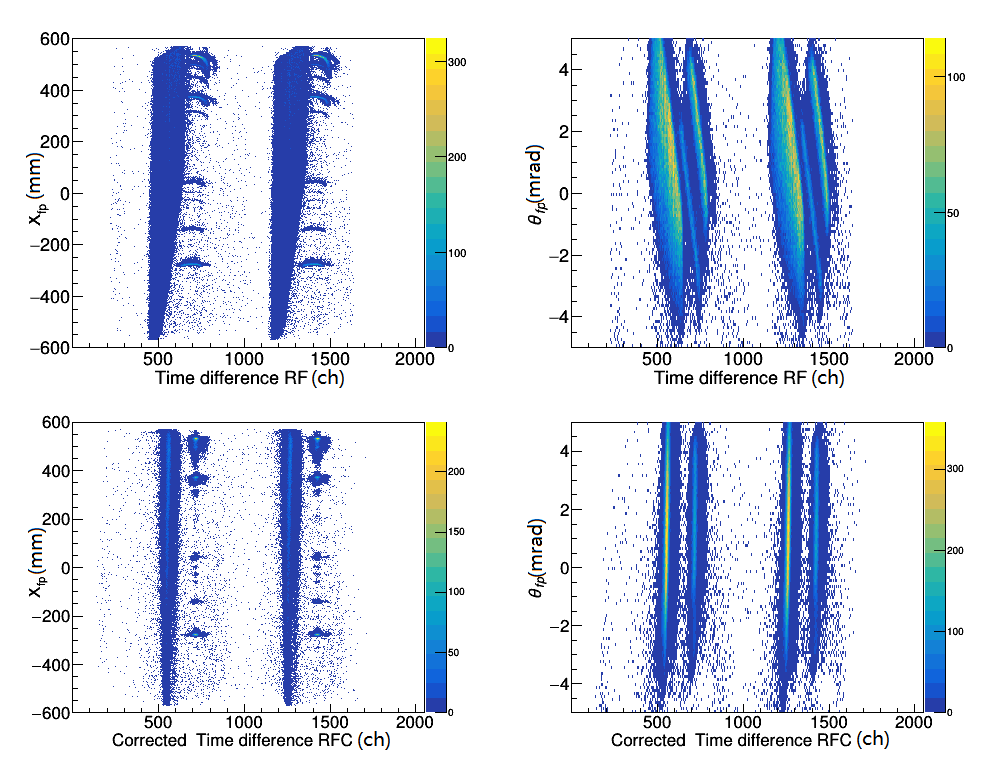
\includegraphics[scale=0.6]{graph/ch4/RFC}}
    \caption{The ToF (RF) in  the top panel and the corrected-ToF (RFC) in the bottom panel for horizontal position and horizontal angle measured at the focal plane. The corrected ToF spectra shows  the dependency on  $x_{fp}$ and $\theta_{fp}$.}
    \label{fig:RFC}
  \end{center}
\end{figure}

An independent method of particle identification is achieved by using the differences of energy losses in the two plastic scintillator detectors. When a charged particle passes through a scintillator, the energy loss depends on its charge and velocity given by the Bethe-Bloch formula:
\begin{equation}
    \label{eq:BB_formula}
    \begin{aligned}
    -\frac{dE}{dx} \propto \frac{az^2}{E}
    \end{aligned}
\end{equation}
where $z$, $a$ and $E$ refer to  the charge, mass and energy, respectively.  The energy loss of a charged particle is approximately proportional to the intensity of the light produced in the scintillator. The photons are collected by PMTs on each side of the scintillator. The number of photons arriving at each PMT depend on the position x and can be expressed in terms of the distance from the PMT $x$  as
\begin{equation}
    \label{eq:intensity}
    \begin{aligned}
    I(x) = I_0 \exp(-\frac{x}{l})
    \end{aligned}
\end{equation}
where $I_0$ is the initially produced light intensity and $l$ is the attenuation length of the scintillator. The mean intensity $I_{mean}$ measured at the left and right side of the PMTs is  expressed as
\begin{equation}
    \label{eq:intensity_mean}
    \begin{aligned}
    I_{mean} = \sqrt{I(x)I(L-x)} = I_0 \exp(-\frac{L}{2l}) \propto \Delta E
    \end{aligned}
\end{equation}
where $L$ is the length of the scintillator. As $I_{mean}$ is independent of the position of the ionization $x$, it is a useful method for particle identification. Fig. \ref{fig:PID} shows an example of particle identification using a cut in the  two-dimensional energy loss versus RFC display.


\begin{figure}[tpb]
  \begin{center}
    \centerline{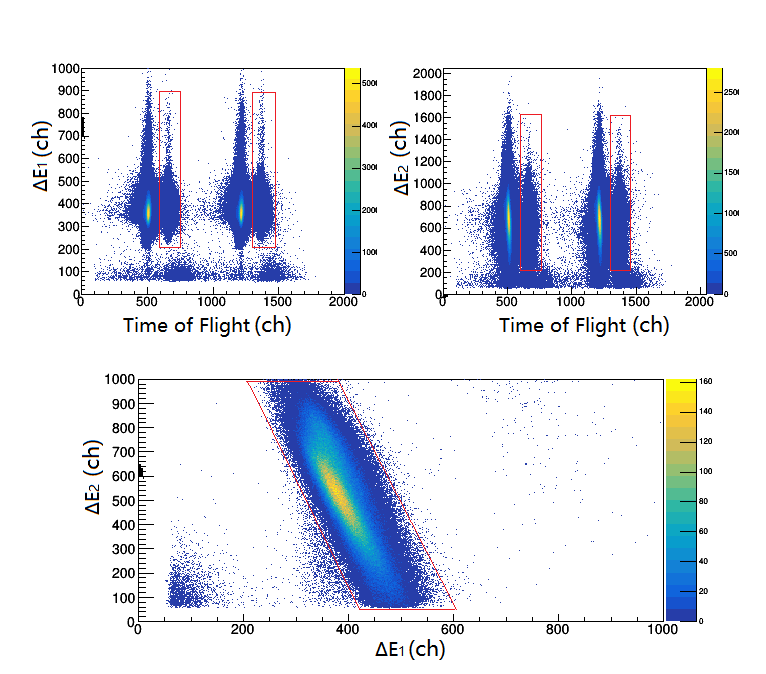
\includegraphics[scale=0.7]{graph/ch4/PID}}
    \caption{Top-left: $\Delta E_1$ vs. ToF plot. Top-right: $\Delta E_2$ vs. ToF cut. Bottom: $\Delta E_1$ v.s. $\Delta E_2$ plot. The red solid lines in these plots were event cuts  used for identifying protons and reducing background particles such as deuterons scattered off the Faraday cups inside the Dipole 1 (D1FC).}
    \label{fig:PID}
  \end{center}
\end{figure}


\section{Track Reconstruction}
As mentioned in the previous chapter, the energy of particles detected in the focal plane is determined using the kinematic equations expressed by scattering positions and angles.
The positions and angles were measured by the MWDCs in  the focal plane, which allows to reconstruct the scattering angle at the target owing to the angular dispersion matching. A voltage of -5000 V was applied to the cathode planes and -500 V to the potential wires in order to optimize the efficiency. The 6 mm spacing of the sense wires for the X-plane and 4 mm spacing for the U-plane were set at ground voltage (Fig. \ref{fig:XUplane} shows the MWDC configuration). The MWDC is designed in such a way that  the electrons, which are produced along the trajectory of a charged particle passing through, drift at a constant velocity  towards the anode under the electric field  between the cathode planes and anode wires, except for the regions nearest to the sense wire. The electrons are collected at the anode wires, generating a negative signal. Particles pass through the MWDCs at about 45$^{\circ}$ and deposit charge on 3 or 4 sense wires, called hits, as shown in Fig. ~\ref{fig:MWDCs}. In the case of a hit with three wires, the focal plane position $p$ is given by
\begin{equation}
    \label{eq:position}
    \begin{aligned}
    p=p_i+d_{sw}\frac{d_{i-1}+d_{i+1}}{d_{i-1}-d_{i+1}}
    \end{aligned}
\end{equation}
where $|d_i|$ is the minimum drift length in a cluster (adjacent to hit wires) with three wires hits, $p_i$ is the position of the $i$-th wire, $d_{i-1}$ and $d_{i+1}$ are the drift lengths to the neighboring sense wires and $d_{SW}$ is the distance between sense wires. The vertical drift lengths $d_{i-1}$, $d_{i}$, $\cdots$ were determined from the drift time recorded by the Time-to-Digital Converter (TDC) and converted to the drift lengths by drift tables. To cover all the signal wires, these drift  tables were calibrated using a spectrum in a  continuum energy region so that the drift length histogram has a flat distribution (Fig.~\ref{fig:drift_time}).


%---
%\begin{figure}[tpb]
%  \begin{center}
%    \centerline{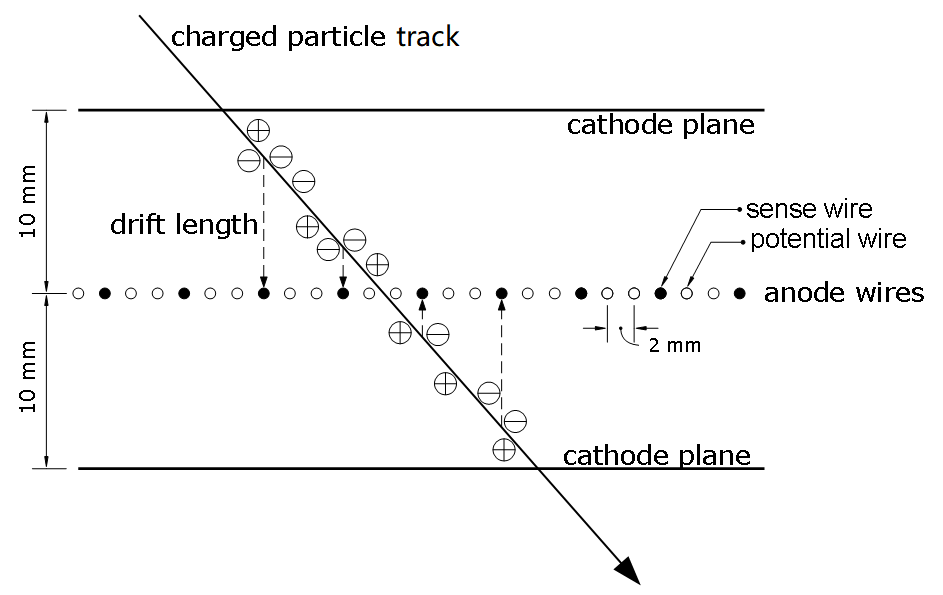
\includegraphics[scale=0.6]{graph/ch4/MWDCs_1}}
%    \caption{X-plane configuration of the MWDC. A sample of the charged particle track is shown together with the cathode planes and anode wires.}
%    \label{fig:MWDCs}
 % \end{center}
%\end{figure}
---%

\begin{figure}[tpb]
  \begin{center}
    \centerline{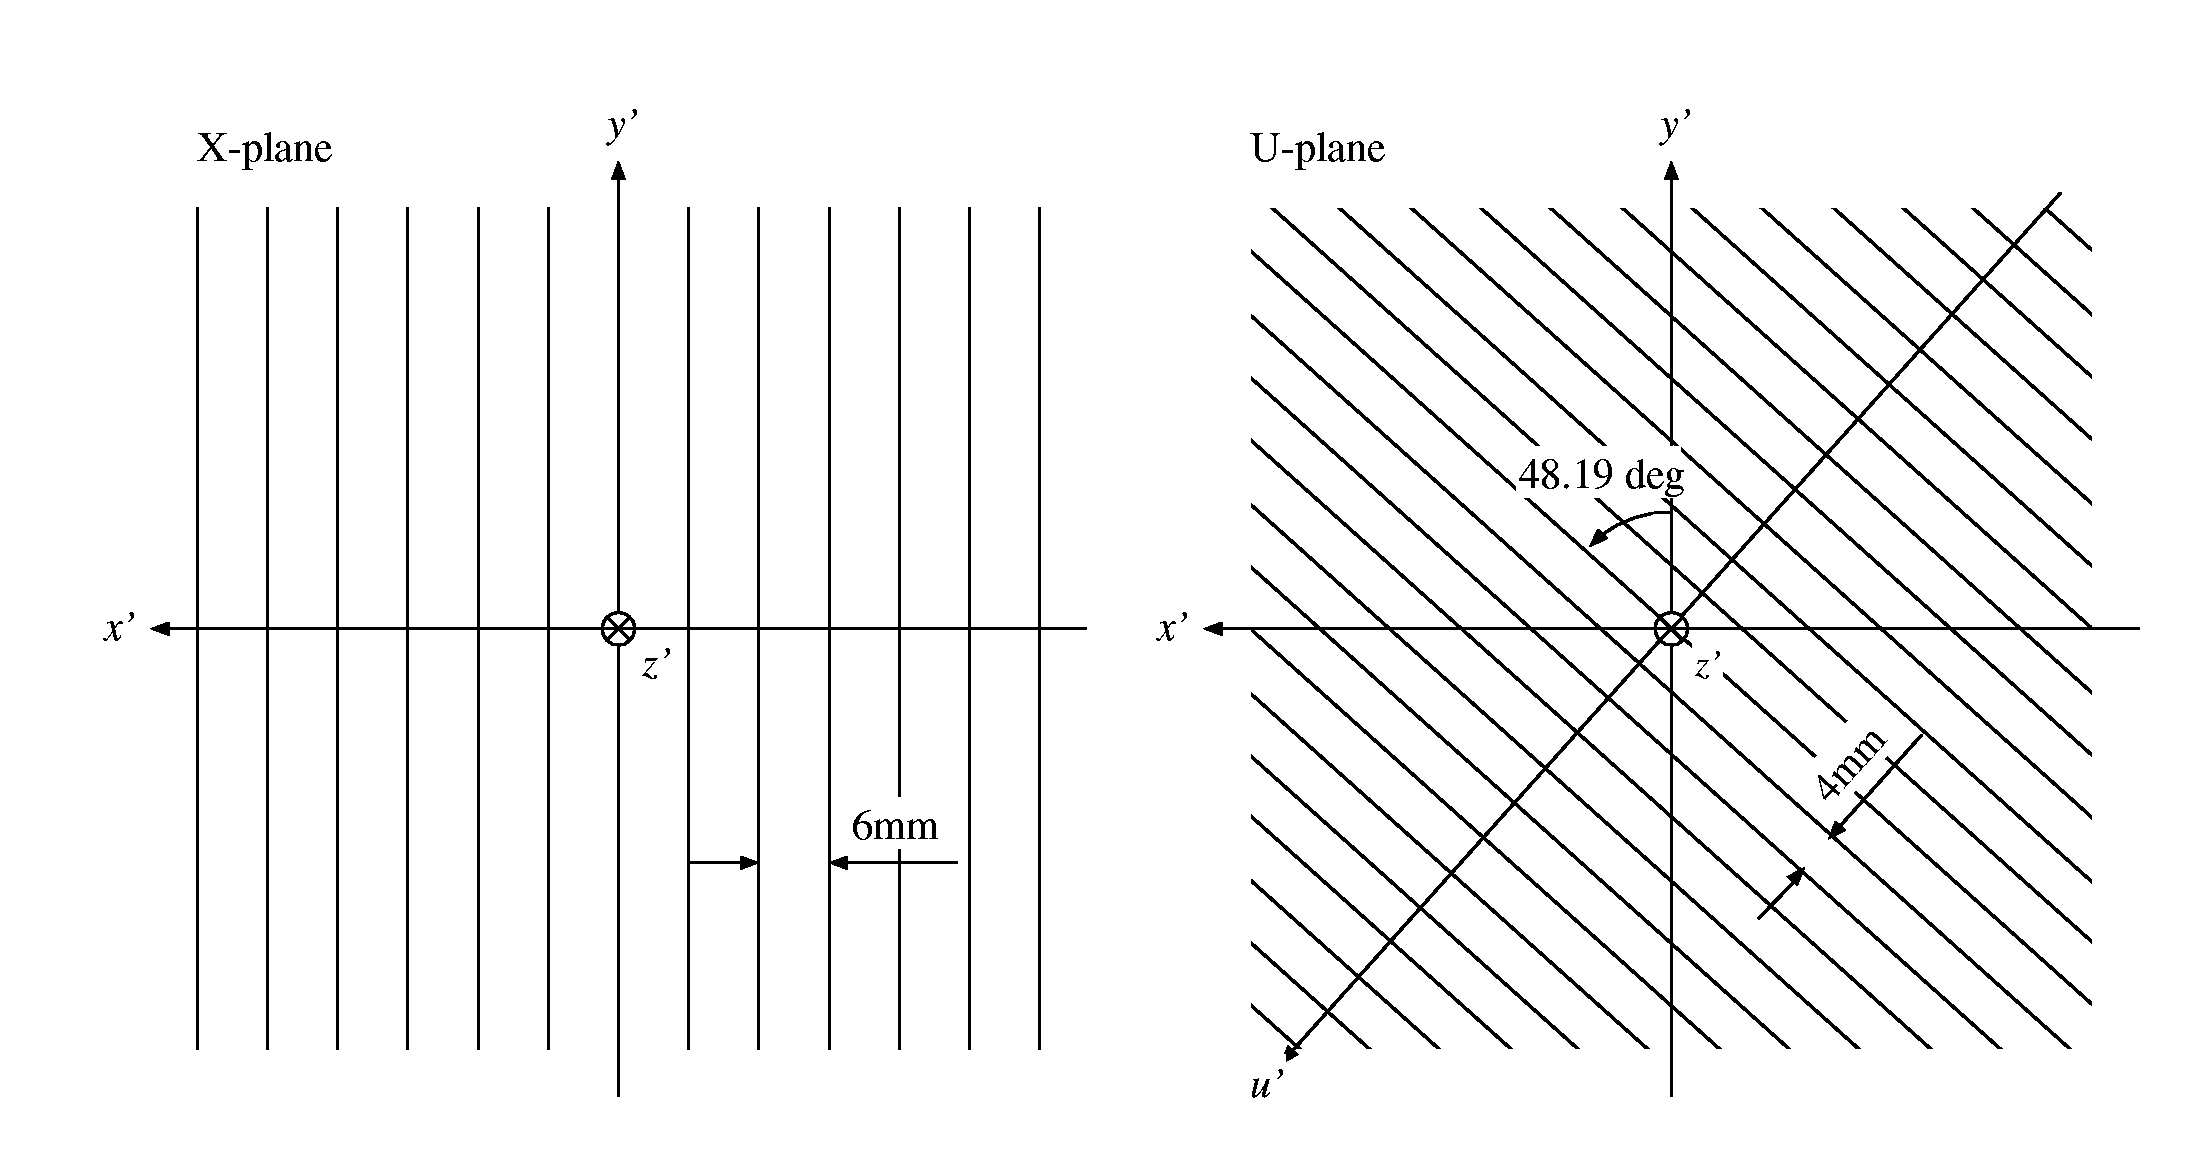
\includegraphics[scale=0.3]{graph/ch4/XUplane}}
    \caption{Wire configuration of the X-plane and U-plane of the MWDC.}
    \label{fig:XUplane}
  \end{center}
\end{figure}

\begin{figure}[tpb]
  \begin{center}
    \centerline{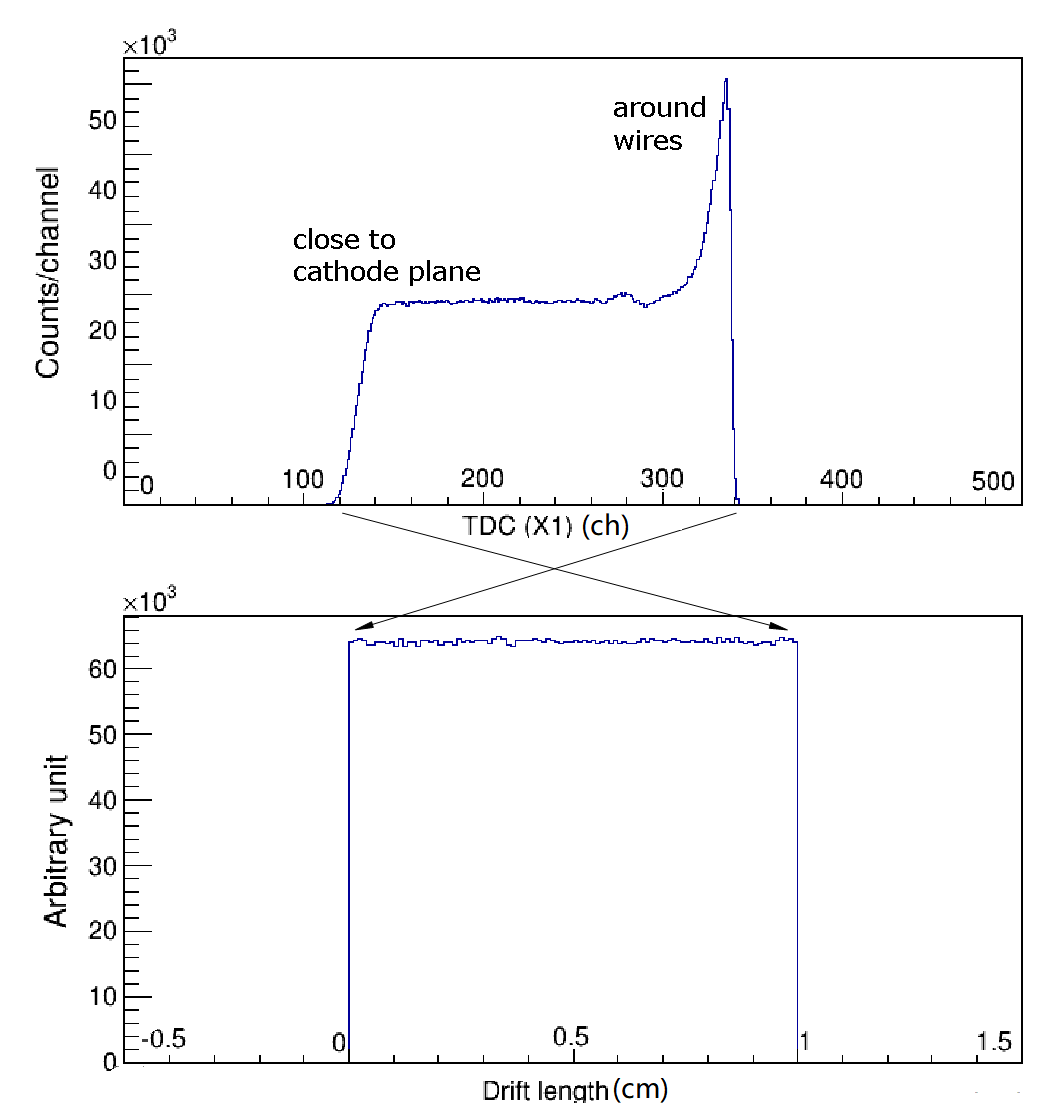
\includegraphics[scale=0.5]{graph/ch4/drift_time}}
    \caption{Conversion of the drift-time spectrum to the drift length for the position measurement with the MWDC. Example from the X-plane.}
    \label{fig:drift_time}
  \end{center}
\end{figure}

The efficiency of X1 wire plane was determined by
\begin{equation}
    \label{eq:efficiency}
    \begin{aligned}
    \eta_{X1} = \frac{N_{U1\cap X2\cap U2}}{N_{X1 \cap U1 \cap X2\cap U2}}
    \end{aligned}
\end{equation}
where $N_{X1 \cap U1 \cap X2\cap U2}$ refers to the number of events detected in all the four wire planes, and $N_{U1\cap X2\cap U2}$ is the number of events detected in the other three wire planes. The total MWDC efficiency is the product of the efficiencies of all anode wire planes:
\begin{equation}
    \label{eq:efficiency}
    \begin{aligned}
    \eta_{MWDC} = \eta_{X1} \times \eta_{X2} \times \eta_{U1} \times \eta_{U2}
    \end{aligned}
\end{equation}
In this experiment, the efficiencies for each wire plane was 96\% and the total efficiency was 85\%.



\section{Scattering Angle Reconstruction}


%%%%%%%%%%%%%
As mentioned in Section 3.3, the scattering angle of the reaction at the target $\Theta_{scatt}=\sqrt{\theta_{tgt}^2 + \phi_{tgt}^2}$ can be reconstructed from the measurement in the focal plane if the angular dispersion matching condition in horizontal direction and the off-focus mode in vertical direction  are realized, where $\theta_{tgt}$  and $\phi_{tgt}$ refer to the horizontal and vertical scattering angles, respectively. In order to calibrate the relationship between the scattering angle and the focal plane measurements, a multi-hole slit called the ``sieve-slit" (shown in Fig.\ref{fig:sieve_slits}) was placed 585 mm downstream of  the target  while the Grand Raiden spectrometer was set to 10$^{\circ}$. A gold target $^{197}Au$ with the thickness of 1.68 $mg/cm^2$ and a carbon target with a thickness of 1 $mg/cm^2$ were used in order to give spectra that cover the full range of the X-focal plane positions $x_{fp}$. The horizontal and vertical scattering angles were well defined by the geometry of the sieve-slit with respect to the target by the reactions $^{197}$Au(d,d')$^{197}$Au and $^{12}$C(d,p)$^{13}$C, respectively. As  shown in the left panel of Fig.\ref{fig:anglecalib}, the image of the sieve-slit can be seen in the focal plane by the vertical focal plane position ($y_{fp}$) versus horizontal focal plane angle ($\theta_{fp}$) for a given range of the X-focal plane position ($x_{fp}$). With the measured $x_{fp}$ and $\theta_{fp}$ from the 2-dimensional plots of images of the sieve-slit, the horizontal scattering angle $\theta_{tgt}$ was calibrated from the $x_{fp}$ and $\theta_{fp}$ dependent equation:
\begin{equation}
    \label{eq:theta_calib}
    \begin{aligned}
        \theta_{tgt} =  \sum_{i=0}^{2} \sum_{j=0}^{2}  a_{ij} \theta_{fp}^i  x_{fp}^j
    \end{aligned}
\end{equation}
The same method was used for  the vertical scattering angle $\phi_{tgt}$ calibration by the $x_{fp}$, $\theta_{fp}$ and $y_{fp}$ dependent equation:
\begin{equation}
    \label{eq:phi_calib}
    \begin{aligned}
        \phi_{tgt} = \sum_{i=0}^2 \sum_{j=0}^2 \sum_{k=0}^2 b_{ijk} \theta_{fp}^i x_{fp}^j y_{fp}^k
    \end{aligned}
\end{equation}
\begin{figure}[tpb]
  \begin{center}
    \centerline{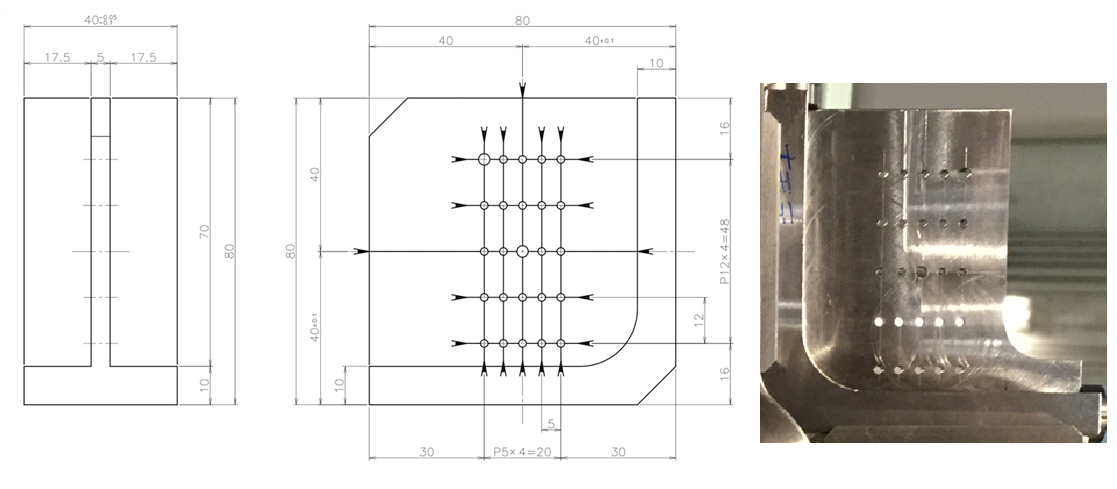
\includegraphics[scale=0.65]{graph/ch4/sieveslits_1}}
    \caption{Drawing (left side) and photograph of the sieve-slit used to calibrate the scattering angles at the target as a function of the measured focal plane angles and vertical positions.}
    \label{fig:sieve_slits}
  \end{center}
\end{figure}
where the fitting parameters $a_{i}$, $b_{i}$ , $c_{ij}$ and $d_{ij}$ were determined by a multi-dimensional non-linear least squares fit. The calibrated scattering angle from the sieve-slit pattern is shown on the right of the Fig.\ref{fig:anglecalib} as the horizontal angle versus the vertical angle. By applying the calibration equations \ref{eq:theta_calib} and \ref{eq:phi_calib} to the measurements in the focal plane ($x_{fp}$, $\theta_{fp}$ and $y_{fp}$), the horizontal and vertical components of scattering angles of the reaction products can be correlated to the target coordinates, which allows for the determination of the excitation energies populated in the recoil nucleus (parameters listed in Table.~\ref{tb:sieve-slit}).

\begin{figure}[tpb]
  \begin{center}
    \centerline{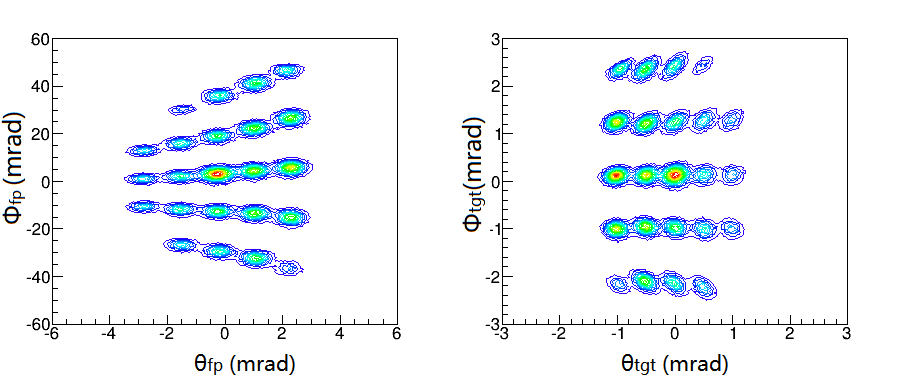
\includegraphics[scale=0.8]{graph/ch4/angle_cal}}
    \caption{2D histogram of the angular calibration run with the sieve-slit. Left panel: measurement of the vertical focal plane position ($y_{fp}$) versus horizonal angle ($\theta_{fp}$). Each blob is associated with a hole of the sieve-slit. Right Panel: reconstructed pattern at the target position after the angular calibration. Data from $^{197}$Au(d,d��)$^{197}$Au at 10$^{\circ}$.}
    \label{fig:anglecalib}
  \end{center}
\end{figure}



\begin{table}[tpb]
    \setlength{\capwidth}{0.7\textwidth}
    \begin{center}
       \caption{TABLE OF THE PARAMETERS $a_{ij}$ AND $b_{ijk}$ DETERMINED IN EQS.\ref{eq:theta_calib} AND \ref{eq:phi_calib}, RESPECTIVELY.}
       \label{tb:sieve-slit}
       \begin{tabular}{cc||cc|cc|cc}
	\hline
    \hline

    $ij$ & $a_{ij}$     & $ijk$ & $b_{ijk}$ & $ijk$ & $b_{ijk}$  & $ijk$  & $b_{ijk}$  \\
    \hline
     00  &  -2.951E+00  & 000    & -2.085E+00    &  100  &  -6.087E-01     &  200   &    2.110E-02                    \\
     01  &  6.903E+00   & 001    &  1.400E+00    &  101  &  -1.806E-01     &  201   &    1.910E-02                      \\
     02  &  4.812E-02   & 002    &  8.200E-05    &  102  &  4.091E0-05     &  202   &    1.040E-07          \\
     10  &  -2.115E-02  & 010    &  5.009E-05    &  110  &   5.000E-04     &  210   &    -3.000E-04                   \\
     11  &   2.217E-04  & 011    &  -9.012E-04   &  111  &   -3.012E-4     &  211   &    2.000E-05                   \\
     12  &   7.200E-06  & 012    &  1.031E-08    &  112  &   2.001E-07     &  212   &    2.011E-08                 \\
     20  &  -4.524E-06  & 020    &  -1.030E-06   &  120  &   8.052E-07     &  220   &    -7.000E-07                 \\
     21  &  -9.142E-08  & 021    &  3.338E-07    &  121  &   -2.019E-07    &  221   &    6.039E-08             \\
     22  &  2.694E-10   & 022    &  1.100E-09    &  122  &   7.008E-08     &  222   &    -8.000E-09                \\

       \hline
       \hline
       \end{tabular}
     \end{center}
\end{table}



\section{Software Corrections  of Higher Order Aberrations}

Besides the energy spread of the incident beam  that were corrected for the full dispersion matching conditions, there are several additional effects (higher order aberration) that need to be corrected  in order to achieve the best possible resolution.
From the reaction kinematics, it is known that particles emitted from the target at the same excitation energy of residual nucleus with different scattering angles will have different momenta $p = B\rho$ and, therefore different  magnetic rigidities $B\rho$, along with the optical aberrations,  both together hindering the spectrum resolution, especially for large angular acceptances.
These effects can be seen in the $\theta_{tgt}$ versus $x_{fp}$ plot shown on the left two panels in Fig~\ref{fig:software}. Each discrete line with curvature indicates a  state of $^{13}$C populated by the $^{12}$C(d,p)$^{13}$C reaction at 0.5$^\circ$. If projecting each curved line of events down onto the x-position, it will affect the width of the corresponding states, which is the resolution of the spectrum. Scattering particles  with larger angles are transported to the focal plane away from the scattering angle.  This creates the higher order aberrations.

The multipole magnet (MP) of Grand Raiden can be used to correct these aberration, but this  is a time consuming procedure and requires precious beam time. Therefore, to correct the kinematic effect and other higher order aberrations, software corrections were performed by straightening each discrete curved state on the 2-dimensional plots $\theta_{tgt}$ versus $x_{fp}$ and  $\phi_{tgt}$ versus $x_{fp}$ around the value of the central ray ($x_{fp}(\theta_{tgt}=0,\phi_{tgt}=0)$ in this case) using mathematical functions. The correction parameters can be determined by employing the fourth-order polynomial function:
\begin{equation}
    \label{eq:software_theta}
    \begin{aligned}
  x_{fp}'=\sum_{i=0}^2 \sum_{j=0}^4 a_{ij} x^i_{fp} \theta^j_{tgt}
    \end{aligned}
\end{equation}
and
\begin{equation}
    \label{eq:software_phi}
    \begin{aligned}
  x_{fp}''=\sum_{i=0}^2 \sum_{j=0}^4 b_{ij} x'^i_{fp} \phi^j_{tgt}
    \end{aligned}
\end{equation}
The top right plot on Fig~\ref{fig:software} shows the 2-dimensional spectrum $\theta_{tgt}$ versus $x'_{fp}$ where $x'_{fp}$ is the corrected focal plane position given by Eq~\ref{eq:software_theta}. In the analysis the horizontal component of the scattering angle was first corrected with Eq~\ref{eq:software_theta}, followed by the vertical scattering angle correction with Eq~\ref{eq:software_phi}. This procedure allowed to improve the final resolution  from 32 keV to 23 keV at 0.5$^{\circ}$ measurements.
%%%%%%%%%%%%%%%%%%%%%%%%%%%%%%%%%%%%%%%%%%%%%%%%%%%%%%%%%%%%%%%%%%%%%%%%%
\begin{figure}[tpb]
  \begin{center}
    \centerline{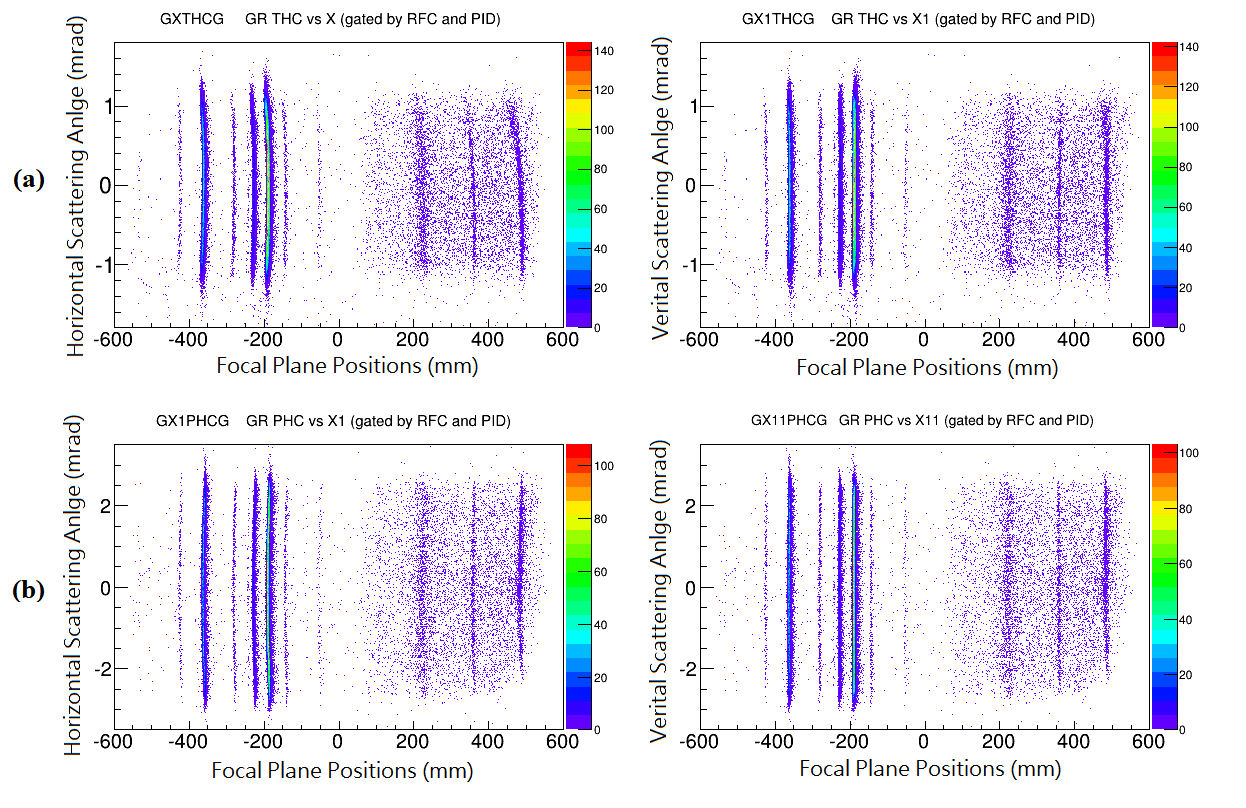
\includegraphics[scale=0.6]{graph/ch4/software}}
    \caption{Software corrections. Example of $^{12}$C(d,p)$^{13}$C at 0.5$^{\circ}$ (a) and (b): plots of the horizontal scattering angle $\theta_{scatt}$ and the vertical scattering angle $\phi_{scatt}$ versus the position in the focal plane before and after correction.}
    \label{fig:software}
  \end{center}
\end{figure}



% % uncomment the following lines,
% if using chapter-wise bibliography
%
% \bibliographystyle{ndnatbib}
% \bibliography{example}

%
%
% Chapter Five
%


\chapter{DATA ANALYSIS}
As mentioned in the previous chapter, focal plane spectra of $^{26}$Mg were taken at three different
magnetic field settings. With overlapping spectra appropriate for energy calibrations for all  states in $^{26}$Mg from the first excited state up to 12.311 MeV excitation energies have been measured. Following the procedure of peak fitting and peak identification,   $^{26}$Mg states were identified in the proton spectra from the reaction $^{25}$Mg(d,p)$^{26}$Mg, extracted with best possible resolution  and  cross sections  and angular distributions were determined.
By comparison with previous work, the spin-parity of the excited states of $^{26}$Mg measured in this work were determined.

\section{Peak Identification}

Fig.~\ref{fig:brho} shows the rigidity B$\rho$ ranges of the three spectrometer settings of the (d,p) reaction at 56 MeV incident energy in the regions of interest. Also shown are the (d,p) reactions on $^{16}$O, $^{12}$C and $^{24}$Mg. These contaminants  were the dominant sources of background that could  show up in the $^{26}$Mg spectra. One method used to identify these contaminant was to perform measurements at different angles, allowing the identification due to the different kinematic shifts (illustrated in Fig.~\ref{fig:K}).
Another method applied was to use  Mylar  and  $^{24}$Mg to obtain
$^{13}$C, $^{17}$O and $^{25}$Mg spectra at the same
magnetic field settings that were used for the
$^{25}$Mg target measurements. Once the peak positions of all the possible contaminants were obtained, these contaminants could be identified in the $^{26}$Mg spectra (shown in Fig.~\ref{fig:peaks}).
%The second method is shown in Fig.\ref{fig:peaks}

\begin{landscape}
    \begin{figure}[tpb]
    \centerline{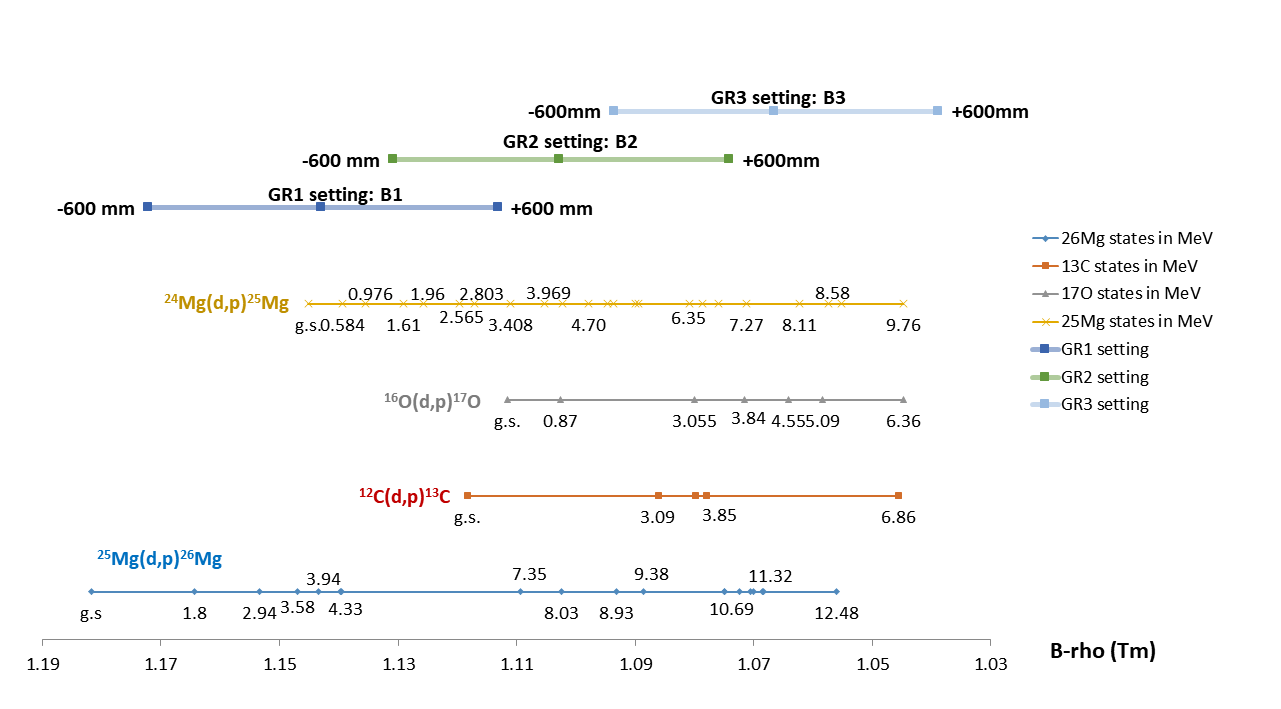
\includegraphics[scale=0.8]{graph/ch5/brho}}
    \caption{B-rho map for the measured three spectrometer settings.}
    \label{fig:brho}
    \end{figure}
\end{landscape}

\begin{figure}[tpb]
  \begin{center}
    \centerline{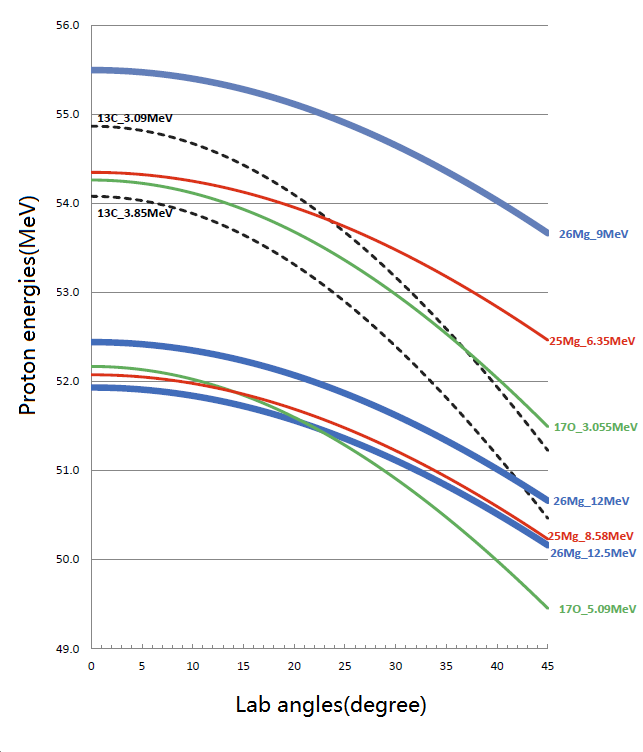
\includegraphics[scale=0.6]{graph/ch5/K}}
    \caption{Kinematic calculation of possible reaction products by proton energies versus  lab angles. Excited states of different targets could be identified by their different angular dependencies.}
    \label{fig:K}
  \end{center}
\end{figure}


\begin{figure}[tpb]
  \begin{center}
    \centerline{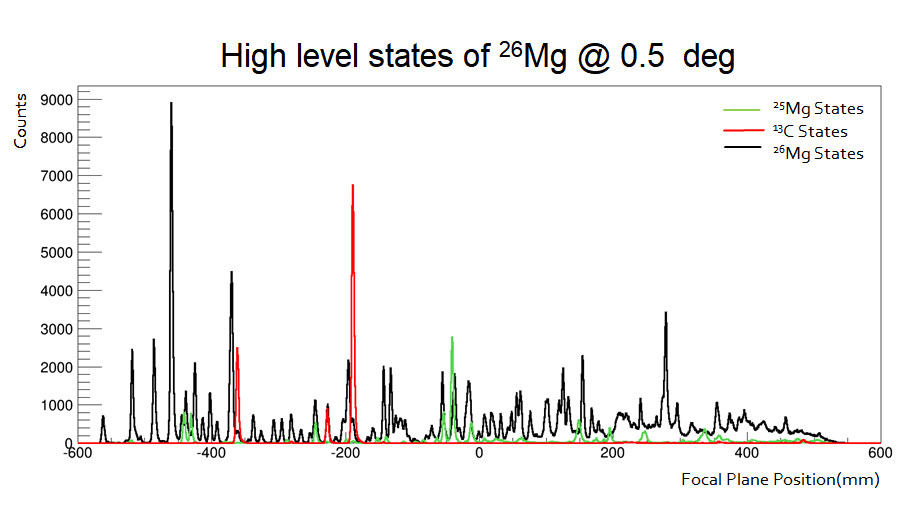
\includegraphics[scale=0.7]{graph/ch5/peaks}}
    \caption{Spectrum showing $^{12}$C(d,p)$^{13}$C, $^{24}$Mg(d,p)$^{25}$Mg and $^{25}$Mg(d,p)$^{26}$Mg for the third GR setting (B3). Energy range is from 8.5 MeV to 13 MeV.}
    \label{fig:peaks}
  \end{center}
\end{figure}

Peak normalization was performed in order to determine the contribution of each contamination peak in the $^{26}$Mg spectrum. This was done by first normalizing the spectrum with respect to the beam charges collected in each run. Then  the $^{26}$Mg spectrum was further improved by removing the identified contaminants. 



In this work all the contamination peaks had almost negligible contribution to the
$^{26}$Mg peaks.

\section{Peak Fitting}
To determine the centroid of each peak, the Right-skewed Gaussian function  was used to fit peaks as it gave lower reduced $\chi^2$ compared to a pure Gaussian shape. Right-skew rather than left-skew  was used because an electron energy shift occurs regularly toward the lower energies side, due to the incomplete charge collection in the detector. The formalism for a Right-skewed Gaussian function is defined as
\begin{equation}
    \label{eq:right_skew_gaus}
    \begin{aligned}
 f(x) & =  A \times \frac{\sqrt{\pi}}{2} \sigma \times RA \times \exp{\left[\left(\frac{\sigma}{2\times RS}\right)^2-\frac{x-x_0}{RS}\right]} \times erfc \left( \frac{\sigma}{RS} - \frac{x-x_0}{\sigma}\right) \\
      & + a x^2 + b x + c
    \end{aligned}
\end{equation}
where

$A$: Amplitude of Gaussian

$\sigma$: Gaussian width (Width = FWHM/1.66)

$x_0$: Position of the Gaussian centroid

$RA$: Right-skew amplitude relative to that of Gaussian

$RS$: Right-skew slope

$erfc$: Standard complementary error function

$a$, $b$, and $c$: Parameters of the second order polynomial background function.
Fig.~\ref{fig:fitting} shows an example of the total fit and the associated individual components obtained using Eq.~\ref{eq:right_skew_gaus}. %Table~\ref{tb:high} lists the energies of states of interest above the neutron threshold together with the the possible spin-parity values.
The Gaussian width $\sigma$ for $^{26}$Mg peaks populated by the $^{25}$Mg(d,p)$^{26}$Mg reaction was fixed for spectra at the same spectrometer angle settings.

\begin{figure}[tpb]
  \begin{center}
    \centerline{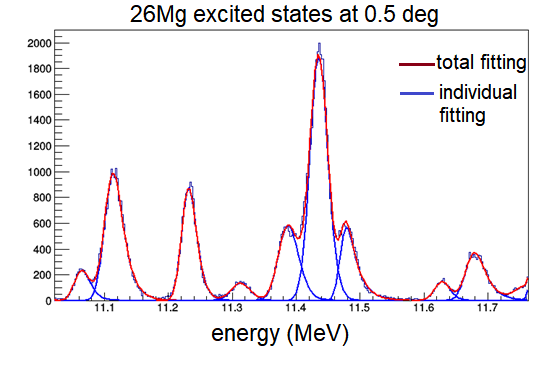
\includegraphics[scale=0.8]{graph/ch5/fitting}}
    \caption{Example of fitting results from Eq.~\ref{eq:right_skew_gaus}. Data from high-lying states of $^{26}$Mg at 0.5$^{\circ}$}
    \label{fig:fitting}
  \end{center}
\end{figure}

%x_error
The error of the peak position measurement consists of the systematic error given by  the peak fitting($\Delta x_{fit}$) and the statistical error ($\Delta x_{stat}$) due to the limited counting numbers defined by
\begin{equation}
    \label{eq:x_stat}
    \begin{aligned}
       \Delta x_{stat} = \frac{FWHM}{\sqrt{N}},
    \end{aligned}
\end{equation}
where $N$ is the integral of counts under each fitted peak. The total error of the peak position is calculated by the square root sum of the two components:
\begin{equation}
    \label{eq:x_error}
    \begin{aligned}
       \Delta x = \sqrt{\Delta x^2_{fit} + \Delta x^2_{stat}}.
    \end{aligned}
\end{equation}

\section{Energy Calibration}

The energy calibration was established using the $^{25}$Mg(d,p)$^{26}$Mg reaction at 0.5$^{\circ}$. The low-lying excited states of $^{26}$Mg are well-known\citep{Cujec1964} so their positions on the focal plane can be used to perform the absolute excitation energy calibration  as shown in Fig.\ref{fig:brho}.

As scattered particles travel through the Grand Raiden (GR) spectrometer, their bending radii in the magnetic dipole  field depend on the momentum following the equation:
\begin{equation}
    \label{eq:brho}
    \begin{aligned}
       B\rho = \frac{p}{q},
    \end{aligned}
\end{equation}
where $B$ is the magnetic field of the GR setting, $\rho$  the orbital radius, and $p$ and $q$  the momenta and the charge states of the scattered particle, respectively. $B\rho$ is  the magnetic rigidity of the detected particles and is associated with the focal plane position ($x_{fp}$). The excitation energy of the residual nuclei can be calculated by solving the two-body scattering kinematics Eq. \ref{eq:kinematic} once $B\rho$ and $q$ are known.
\begin{equation}
    \label{eq:kinematic}
    \begin{aligned}
 E_x = & \left(  { m^2_{in} + m^2_{tar} + m^2_{out} + 2E_{in}m_{tar}-2E_{out}m_{tar}}  \right. \\
       & \left.  { -2 E_{in}E_{out}+2p_{in}p_{out}\cos\theta_{lab} }        \right) ^{1/2} -m_{res} \\
    \end{aligned}
\end{equation}
where $m_{in}$, $m_{tar}$, $m_{out}$ and $m_{res}$ are the masses of the incident beam, target nuclei, outgoing particles and the residual nuclei, respectively. $E_x$, $E_{in}$ and $E_{out}$ are the energies of the excited states, incident  particles and outgoing particles, respectively. $p_{in}$, $p_{out}$ and $\theta_{lab}$ are the momenta of the incident and outgoing particles and the scattering angles in the lab frame. Since the energy losses of particles in the target need to be taken into account in the kinematic calculations, it is assumed that on average the $^{25}$Mg(d,p)$^{26}$Mg occurs at the center of the target. Therefore, the kinematic terms $E_{in}$, $E_{out}$, $p_{in}$ and $p_{out}$ were determined by the following equations:
\begin{equation}
    \label{eq:kinematic2}
    \begin{aligned}
        E_{in}  = m_{in} + T_{in} - E_{loss1} \\
        E_{out} = \sqrt{m_{out}^2 + p^2_{out}} + E_{loss2} \\
        p_{in}  = \sqrt{E_{out}^2-m_{in}^2}   \\
        p_{out} = \sqrt{E_{out}^2 - m_{out}^2}
     \end{aligned}
\end{equation}
where $E_{loss1}$ and $E_{loss2}$ refer to the energy loss of deuterons in the target prior to the reaction, and the protons after the reaction, respectively. This was calculated by the Stopping and Range of Ions in Matter (SRIM) program\citep{srim}. $T_{in}$ represents the kinematic energy of the incident beam. $p_{out}$ is the momentum of the scattered particles whose movements are described by Eq. \ref{eq:brho}. Therefore, once the magnetic rigidities of the detected particles in the focal plane are known, the excitation energies of the corresponding recoil nuclei can be calculated.

To determine the relationship between the measured $x_{fp}$ and $B\rho$, a function quadratic in $x_{fp}$ was used. In addition, as mentioned in the previous section,  three spectrometer  settings were used by changing the magnetic fields with sufficient overlap between the different spectra.

Finally, the calibration function is following the form:
\begin{equation}
    \label{eq:focal_plane_cali}
    \begin{aligned}
    B\rho /B\rho_0 = (ax_{fp}^2+bx_{fp}+c)/( 1.1597 \ T\cdot m)
    \end{aligned}
\end{equation}
where $x_{fp}$ is the corrected focal plane position after the software corrections. The quantity  1.1597 $T\cdot m$ is the magnetic rigidity of the first excited state of $^{26}$Mg.

The focal plane calibration obtained above is derived from the well-known low-lying states of $^{26}$Mg that were populated in the first spectrometer setting (B1). It could not be directly applied to the other two spectrometer  settings, for example, the third setting (B3) that corresponds to the region of our interest. However, since each setting was scaled to the next one, the initial focal plane calibration can also be scaled to the other focal plane settings by using the scaling factors obtained during the experiment:
\begin{equation}
    \label{eq:scaling}
    \begin{aligned}
    B\rho  =  \frac{B_2}{B_1}(ax_{}^2+bx_{}+c).
    \end{aligned}
\end{equation}
where $\dfrac{B_2}{B_1}$ represents the scaling factor between two different settings.



%%%
%b-rho : g.s. 1.1770
%b-rho : 1st  1.1597
\begin{figure}[tpb]
  \begin{center}
    \centerline{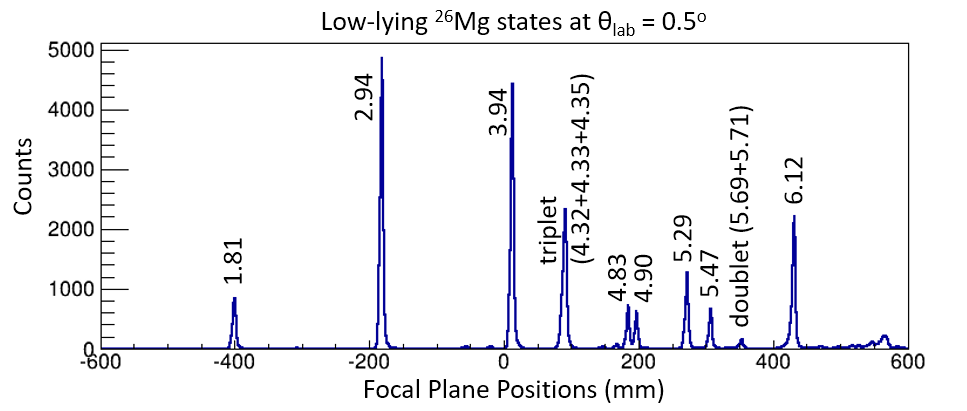
\includegraphics[scale=0.6]{graph/ch5/mg26_low}}
    \caption{Spectrum of low-lying $^{26}$Mg states populated by the $^{25}$Mg(d,p)$^{26}$Mg reaction at $\theta_{lab}$ = 0.5$^{\circ}$ under the first spectrometer setting. Level energies are taken from\citep{Cujec1964}}
    \label{fig:lowlying}
  \end{center}
\end{figure}

\begin{table}[tpb]
    \setlength{\capwidth}{0.7\textwidth}
    \begin{centering}
       \caption{WELL-KNOWN STATES USED IN THE ENERGY CALIBRATION}
       \label{tb:wellknown_states}
       \begin{tabular}{c c c}
       \toprule
       \toprule
          Well-known $^{26}$Mg States from NNDC~\citep{NNDC}  & Magnetic Rigidity & Focal Plane Position   \\
         (MeV) &(T $\cdot$ m)& (mm) \\
         \hline
         1.80874(4)  & 1.16429 & -400.691   \\
         2.93833(4)  & 1.15328 & -181.612   \\
         3.94157(4)  & 1.14342 & 12.396   \\
         4.83513(5)  & 1.13458 & 184.390   \\
         4.90144(7)  & 1.13392 & 197.105   \\
         5.29174(6)  & 1.11300 & 271.915   \\
         5.47605(7)  & 1.12819 & 307.048   \\
         6.12547(5)  & 1.12168 & 430.729   \\
         \hline
       \end{tabular}
     \end{centering}
\end{table}

\begin{figure}[tpb]
  \begin{center}
    \centerline{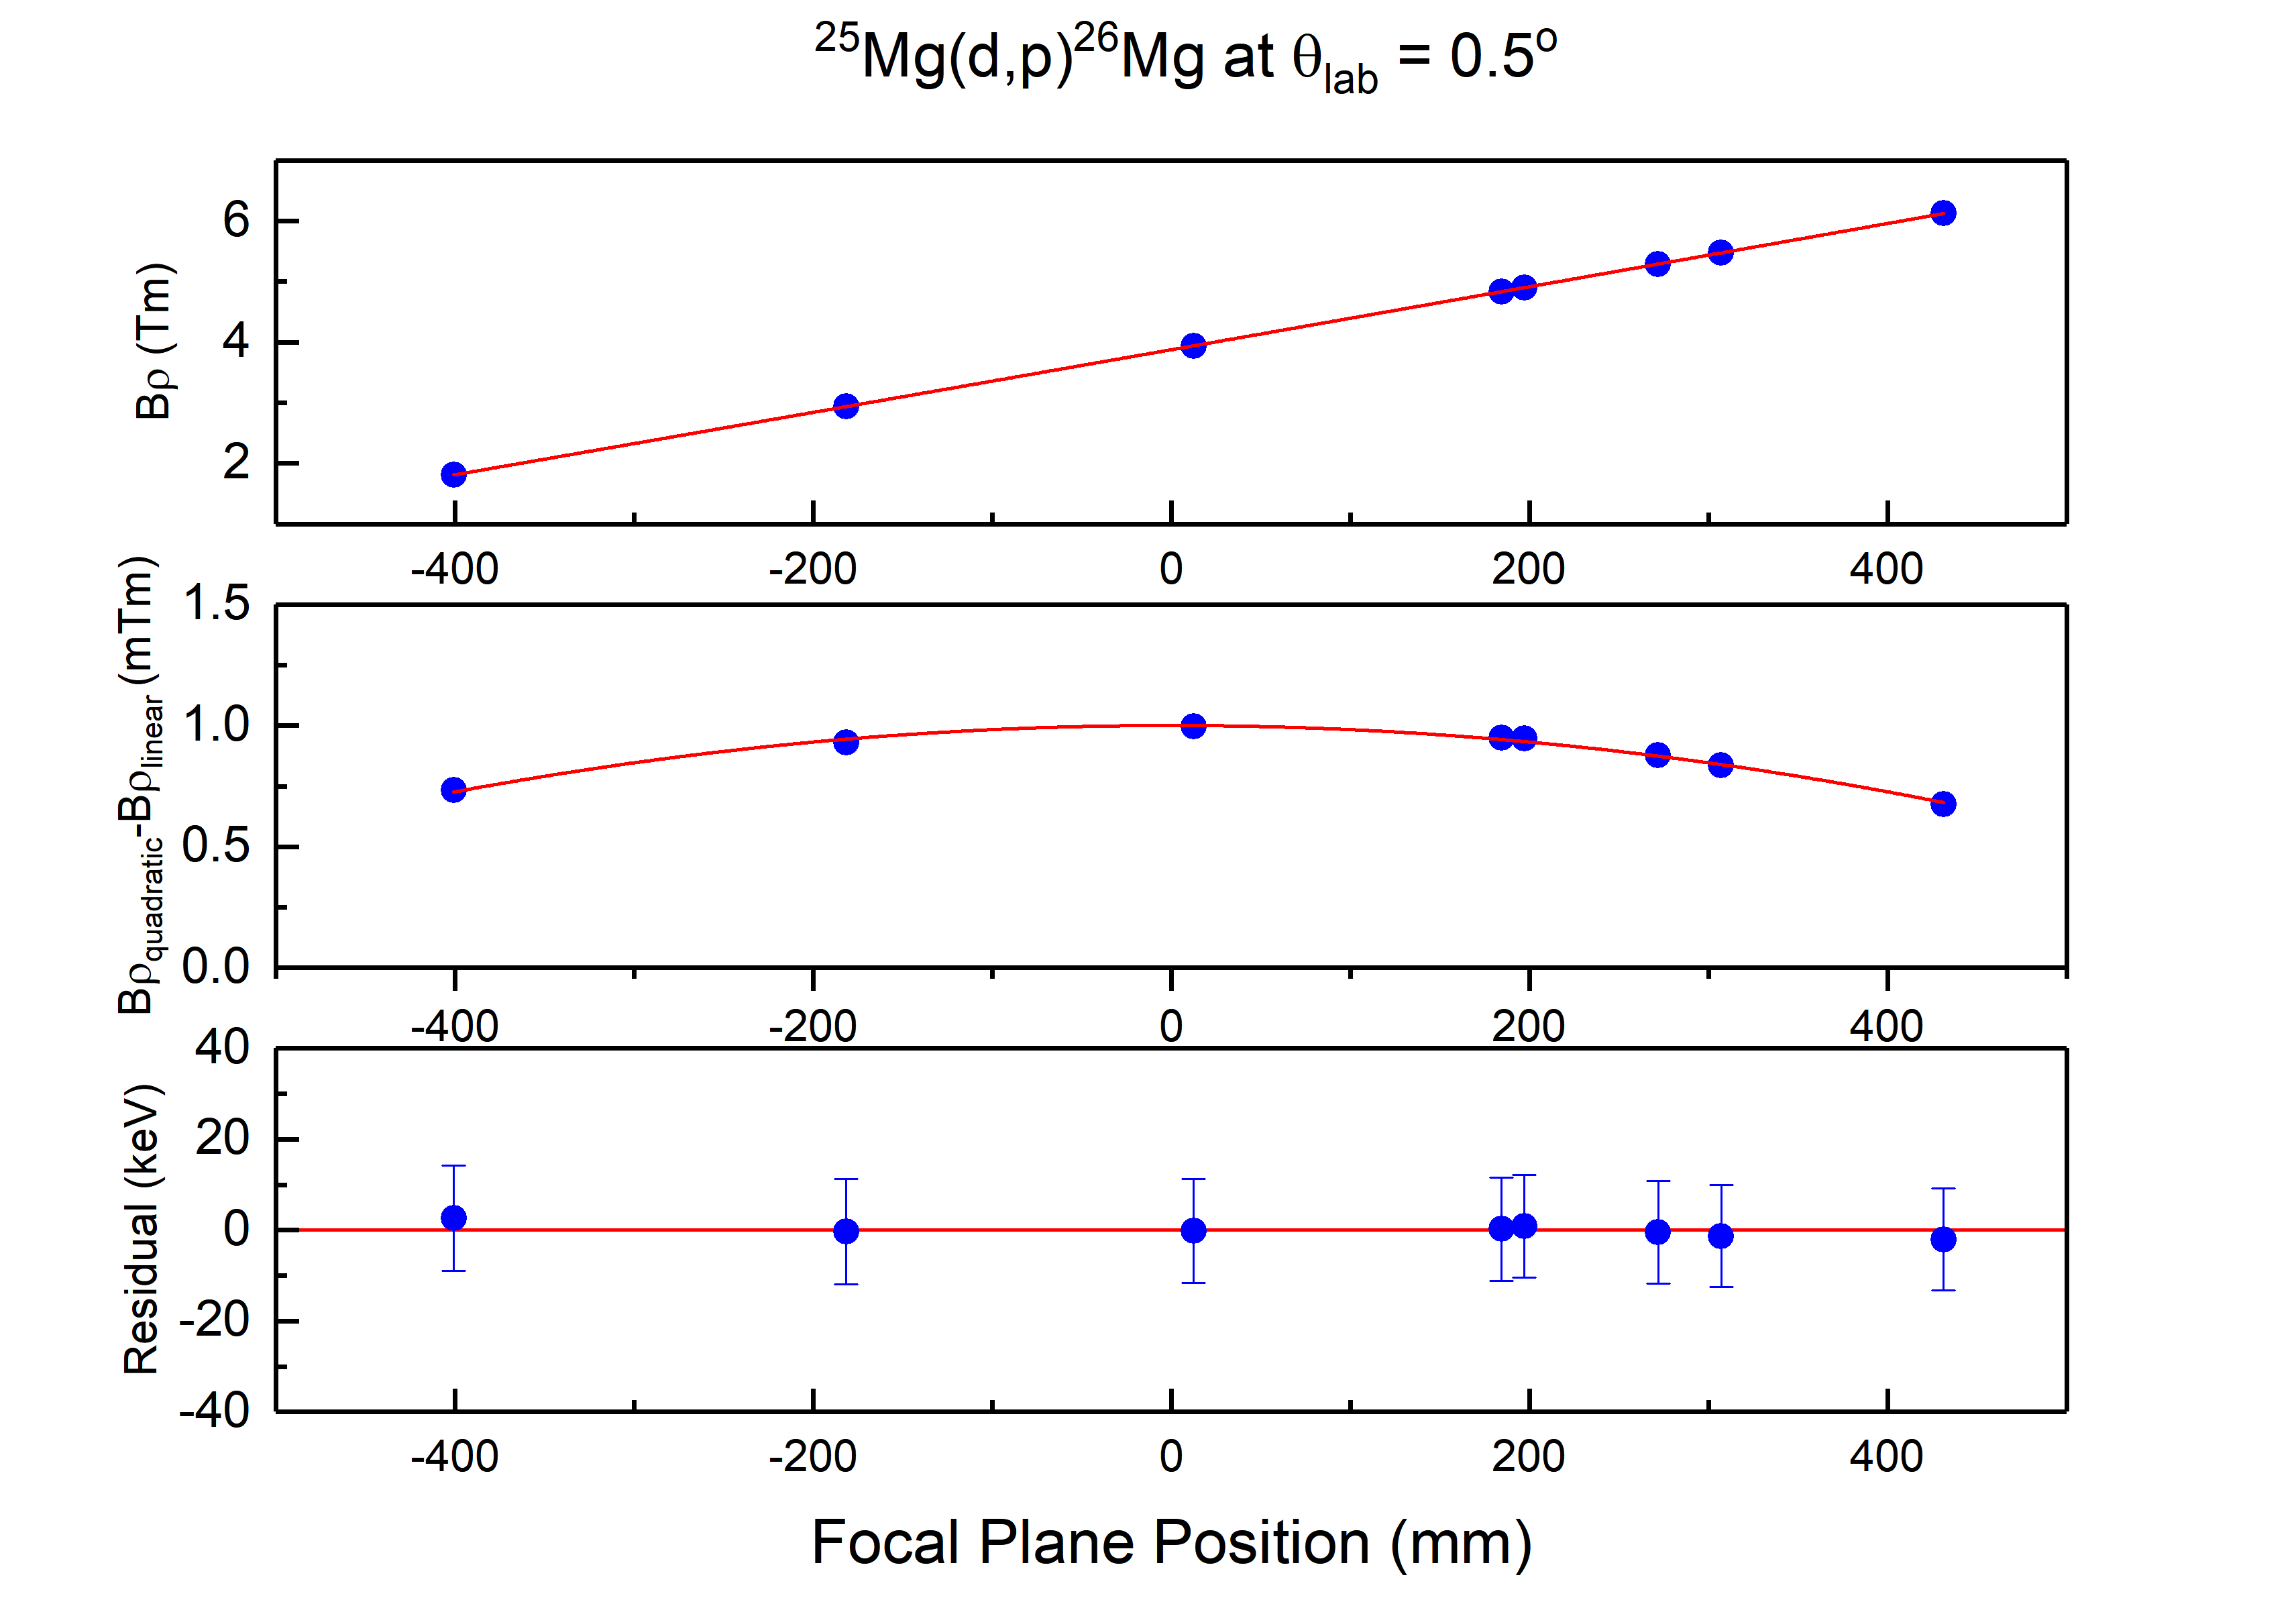
\includegraphics[scale=0.4]{graph/ch5/focalplane}}
    \caption{Focal plane calibration. Top panel: quadratic fitting . Middle panel: quadratic residual of the fit. Bottom panel: The deviation of the calibration from the actual data in terms of energy. }
    \label{fig:fp}
  \end{center}
\end{figure}

The determination of the fitting error of B$\rho$ in Eq. \ref{eq:focal_plane_cali} is  not straightforward since the calibration parameters  $a$, $b$ and $c$ are not  independent. Solving the covariance error matrix gives the systematic error $B\rho_{fit}$ by
\begin{equation}
    \label{eq:b-rho_fit}
    \begin{aligned}
    \delta B \rho^2_{fit} &=   (\frac{\partial B\rho}{\partial a})^2 (\delta a)^2 + (\frac{\partial B\rho}{\partial b})^2 (\delta b)^2 + (\frac{\partial B\rho}{\partial c})^2 (\delta c)^2 \\
                    & + \frac{\partial B\rho}{\partial a} \frac{\partial B\rho}{ \partial b} \delta a \delta b
                     + \frac{\partial B\rho}{\partial a} \frac{\partial B\rho}{ \partial c} \delta a \delta c
                     + \frac{\partial B\rho}{\partial b} \frac{\partial B\rho}{ \partial c} \delta b \delta c    \\
    \end{aligned}
\end{equation}
where $\delta a$, $\delta b$ and $\delta c$ are  covariant matrix terms.

The other type of error in the fitting is the error regarding the peak position:
\begin{equation}
    \label{eq:b-rho_pos}
    \begin{aligned}
    \delta B \rho_{c}^2 &=   (\frac{\partial B\rho}{\partial x})^2 (\Delta x)^2
    \end{aligned}
\end{equation}
where $\Delta x$ is obtained from Eq. ~\ref{eq:x_error}.

The final error of the magnetic rigidities can be expressed as
\begin{equation}
    \label{eq:b-rho_tot}
    \begin{aligned}
    \delta B \rho^2 &= B\rho_{c}^2 + B\rho_{fit}^2 \\
                    &=  (\frac{\partial B\rho}{\partial x})^2 (\Delta x)^2
                     + (\frac{\partial B\rho}{\partial a})^2 (\delta a)^2 + (\frac{\partial B\rho}{\partial b})^2 (\delta b)^2 + (\frac{\partial B\rho}{\partial c})^2 (\delta c)^2 \\
                    & + \frac{\partial B\rho}{\partial a} \frac{\partial B\rho}{ \partial b} \delta a \delta b
                     + \frac{\partial B\rho}{\partial a} \frac{\partial B\rho}{ \partial c} \delta a \delta c
                     + \frac{\partial B\rho}{\partial b} \frac{\partial B\rho}{ \partial c} \delta b \delta c    \\
    \end{aligned}
\end{equation}

The final schematic error of the excitation energy calculated from  Eq. ~\ref{eq:kinematic} was determined by the propagation of the errors from terms that were associated with $E$, including the error of particle energy loss in targets given by SRIM and the error associated with the atomic mass  ~\citep{mass_excess}.


The $^{26}$Mg energy levels in the region of interests populated by the (d,p) reaction are listed in Table~\ref{tb:6Lid}, Table~\ref{tb:aa}, Table~\ref{tb:ddpp}, Table~\ref{tb:dp} and Table~\ref{tb:other}.

\section{Cross Section Calculation}

The differential cross section is defined by
\begin{equation}
    \label{eq:cross_section}
    \begin{aligned}
    \frac{d\sigma}{d\Omega} = \frac{Y}{N_B l N_0 \eta \Delta \Omega}  cm^2/sr
    \end{aligned}
\end{equation}
Where $Y$ is the reaction yields in the accepted solid angle $\Delta \Omega$ (in msr) while $\Delta \Omega$ was calculated from the $\theta_{tgt}$ and $\phi_{tgt}$ plot  and was determined to be  2.79 msr in this experiment.  $\eta$ is the efficiency of the total detection system (85\% in the experiment) as described in the previous chapter.  $N_0$ is the number of target nuclei per cm$^2$ determined from the target thickness $\Delta x$, and $N_B$ is  the total number of incident particles which depends on the integrated current of the incident  beam $Q$, the atomic charge $Z$ and the electron charge $e$. The live time ratio $l$ of the detection system varied from 93\% to 96\%.
%$N_B$ is the number of incident beam particles.

The cross-section measurement near 0$^{\circ}$  required a different Faraday cup compared to those at higher angles. As shown in Fig. 3.8 ( Chapter 3), in the  0$^{\circ}$ measurement the Faraday cup was placed inside the first dipole  D1 (D1FC).  For the angle at 5$^{\circ}$  the Faraday cup Q1FC downstream of the quadrupole  Q1 was used. For larger angles the Faraday cup in the scattering chamber (SCFC) was employed. Measurements at small angles by D1FC and Q1FC need to be normalized to SCFC since SCFC has an effective electron suppression
system. Faraday cup normalization between the different modes was achieved by monitoring the count rate on the D1FC and SCFC for several runs.







\section{Analysis of Energy Levels}

In this measurement of $^{25}$Mg(d,p)$^{26}$Mg, 102 energy levels were populated above the first excited states up to 12.311 MeV.
Considerable effort has been made in the past by various methods to probe the $^{26}$Mg resonances in the astrophysical region of interest. The reaction mechanism of each reaction  focuses on different aspects in terms of the input parameters into the  reaction rate calculation.
The (d,p) reactions used in this work populate more or less every state but the strength depends on the strength of the single particle component in the wave function.
The excited states of $^{26}$Mg in the present work will be compared with  the states populated by several different reactions, including
the reaction $^{22}$Ne($^6$Li,d)$^{26}$Mg by Ugalde $et\ al.$\citep{Ugalde2007}, Giesen $et\ al.$\citep{GIESEN199395} and Talwar $et\ al.$\citep{Rashi2016},
the reaction $^{26}$Mg($\alpha$,$\alpha'$)$^{26}$Mg by Talwar $et\ al.$\citep{Rashi2016} and Adsley $et\ al.$\citep{26mgaa2017},
the inelastic scattering $^{26}$Mg(p,p$'$)$^{26}$Mg and  $^{26}$Mg(d,d$'$)$^{26}$Mg by Adsley $et\ al.$\citep{26mgdd2018} and Moss $et\ al.$ \citep{Moss1967},
the reactions $^{25}$Mg(d,p)$^{26}$Mg by Cujec $et\ al.$\citep{Cujec1964}, Hinds $et\ al.$\citep{Hinds1965}\citep{Hinds1961} and Arciszewski $et\ al.$\citep{Arciszewski1984}, along with data from the n-ToF $^{25}$Mg(n,$\gamma$) measurement by Massimi $et\ al.$\citep{Massimi}\citep{MASSIMI2017},
and the last comparison will be among reactions $^{23}$Na($\alpha$,p$\gamma$)$^{26}$Mg and $^{12}$C($^{18}$O,$\alpha$)$^{26}$Mg by Glatz $et\ al.$\citep{Glatz1986} and Gustafson $et\ al.$ \citep{Gustafson1976}, respectively.
%%%%%%%%%%%%





\subsection{Comparison with the  reaction $^{22}$Ne($^6$Li,d)$^{26}$Mg}

Studies of the $\alpha$-transfer on $^{22}$Ne have been performed \citep{GIESEN199395}\citep{Ugalde2007}\citep{Rashi2016} and several states with strong $\alpha$ structure have been observed and is listed in Table~\ref{tb:6Lid}. These measurements also provided critical information on the $\alpha$-widths for states above the $\alpha$-threshold which contribute to reaction rate calculation for the $^{22}$Ne + $\alpha$ system. Since no  ($\alpha$,n) resonance strength was determined in the $\alpha$-channel in this work,  the data from $\alpha$-transfer data is needed.  Giesen $et\ al.$\citep{GIESEN199395} reported two natural parity resonances (E$_x=$10.694(20) MeV and E$_x=$10.949(25) MeV) between the  $\alpha$- and $n$- thresholds with the resolution of 120 keV.  Ugalde $et\ al.$\citep{Ugalde2007} subsequently improved the resolution to 63 keV in the region of interest.   Talwar $et\ al.$\citep{Rashi2016} observed and used additional resonances to the reaction rate calculation with the resolution of 100 keV.
However, due to the fact that the $\alpha$-transfer reaction only populates natural parity states and favors states with a strong $\alpha$ structure, it  gives a lower number of states comparing to the (d,p) reaction. Other than that, the energy levels in the present work are mostly consistent with  the previous ($^6$Li,d) measurements, despite one weakly populated state E$_x=$11.644(20) MeV in Giesen $et\ al.$'s work is not observed in the present measurements.


%%%%%%%%%%%%%%%%%6Lid

\begin{center}
%\setlength{\LTleft}{0pt} \setlength{\LTright}{0pt}
%\setlength{\tabcolsep}{7mm}
%%   \begin{ThreePartTable}
    \begin{longtable}{cc c cc cc}
    %\setlength{\LTleft}{0pt} \setlength{\LTright}{0pt}
    \caption{COMPARISONS WITH STATES of $^{26}$MG POPULATED BY THE ($^6$LI,D) REACTION \label{tb:6Lid}\/}\\
    \toprule
    \hline
    \multicolumn{2}{c}{This Work}          & Ugalde $et\ al.$\citep{Ugalde2007}    & \multicolumn{2}{c}{Giesen $et\ al.$\citep{GIESEN199395}}  & \multicolumn{2}{c}{Talwar $et\ al.$\citep{Rashi2016}} \\
    \multicolumn{2}{c}{($d,p$)}            &              ($^6Li,d$)               & \multicolumn{2}{c}{($^6 Li,d$)}      & \multicolumn{2}{c}{($^6 Li,d$)}     \\
      $E_x$(MeV)  &  $l_n$                 & $E_x$(MeV)                            &  $E_x$(MeV)   & $J^{\pi}$             & $E_x$(MeV)   & $J^{\pi}$             \\
    \midrule
    \endfirsthead % Everything above goes at the top of the 1st page only
% As with the first header, we don't want obscene amounts of space for
% subsequent headings either, and eliminate an em of whitespace.
  \caption[]{{\em Continued}}\\
    \midrule
    \hline
    \multicolumn{2}{c}{This Work}          & Ugalde $et\ al.$\citep{Ugalde2007}    & \multicolumn{2}{c}{Giesen $et\ al.$\citep{GIESEN199395}}  & \multicolumn{2}{c}{Talwar $et\ al.$\citep{Rashi2016}} \\
    \multicolumn{2}{c}{($d,p$)}            &              ($^6Li,d$)               & \multicolumn{2}{c}{($^6 Li,d$)}      & \multicolumn{2}{c}{($^6 Li,d$)}     \\
      $E_x$(MeV)  &  $l_n$                 & $E_x$(MeV)                            &  $E_x$(MeV)   & $J^{\pi}$             & $E_x$(MeV)   & $J^{\pi}$             \\
    \midrule
    \endhead
    \endfoot % The above section goes at the bottom of continuation pages
  \bottomrule

\endlastfoot

  7.347 (12)    &       &                   &                   &                   &    7.365(13)      &  2$^+$            \\
  7.540 (11)    &       &                   &                   &                   &                   &                   \\
  7.677 (11)    &       &                   &                   &                   &    7.671(16)      &                   \\
  7.712 (12)    &       &                   &                   &                   &                   &                   \\
  7.733 (11)    &       &                   &                   &                   &                   &                   \\
  7.809 (11)    &       &                   &                   &                   &    7.821(22)      &  3$^-$            \\
  7.942 (10)    &       &                   &                   &                   &                   &                   \\
  7.996 (11)    &       &                   &                   &                   &                   &                   \\
  8.042 (11)    &       &                   &                   &                   &    8.040(13)      &   2$^+$           \\
  8.179 (12)    &       &                   &                   &                   &    8.214(14)      &   6$^+$           \\
  8.243 (12)    &       &                   &                   &                   &                   &                   \\
  8.393 (11)    &       &                   &                   &                   &                   &                   \\
  8.454 (10)    &       &                   &                   &                   &                   &                   \\
  8.497 (11)    &       &                   &                   &                   &                   &                   \\
  8.527 (11)    &       &                   &                   &                   &                   &                   \\
  8.621 (11)    &       &                   &                   &                   &    8.625(15)      &   5$^-$           \\
  8.706 (11)    &       &                   &                   &                   &                   &                   \\
  8.865 (11)    &       &                   &                   &                   &                   &                   \\
  8.904 (10)    &       &                   &                   &                   &                   &                   \\
 8.931 (11)     &       &                   &                   &                   &    8.931(13)      &   1$^-$,2$^+$     \\
  8.960 (11)    &       &                   &                   &                   &                   &                   \\
   9.052 (11)   &       &                   &                   &                   &                   &                   \\
  9.167 (11)    &       &                   &                   &                   &                   &                   \\
  9.238 (12)    &       &                   &                   &                   &                   &                   \\
  9.263 (11)    &       &                   &                   &                   &                   &                   \\
   9.322(11)    &       &     9.32(6)       &                   &                   &                   &                   \\
  9.382 (11)    &       &                   &                   &                   &    9.383(16)      &  0$^+$,1$^-$      \\
  9.430 (11)    &       &                   &     9.404(20)     & (4$^+$), 6$^+$    &                   &                   \\
  9.476 (11)    &       &                   &                   &                   &                   &                   \\
   9.578(11)    &       &     9.57(4)       &    9.586(20)      &   4$^+$           &   9.595(32)       &  1$^-$,2$^+$      \\
   9.613(11)    &       &                   &                   &                   &                   &                   \\
  9.683 (10)    &       &                   &                   &                   &                   &                   \\
  9.716 (11)    &       &                   &                   &                   &                   &                   \\
  9.770 (11)    &       &                   &                   &                   &                   &                   \\
  9.856 (11)    &       &                   &                   &                   &                   &                   \\
  9.985 (11)    &       &                   &     9.985(20)     &                   &    9.987(18)      & 1$^-$,2$^+$       \\
  9.991 (11)    &       &                   &                   &                   &                   &                   \\
  10.040(10)    &       &                   &                   &                   &                   &                   \\
  10.100(10)    &       &                   &                   &                   &                   &                   \\
  10.137(11)    &       &                   &                   &                   &                   &                   \\
  10.269(11)    &       &                   &                   &                   &                   &                   \\
  10.320(11)    &       &                   &                   &                   &                   &                   \\
  10.355(12)    &       &                   &     10.335(20)    &   (7$^-$)         &   10.357(14)      & 2$^+$             \\
  10.385(12)    &       &                   &                   &                   &                   &                   \\
  10.487(12)    &       &                   &                   &                   &                   &                   \\
  10.522(11)    &       &                   &                   &                   &                   &                   \\
  10.568(11)    &       &                   &    10.568(25)     &                   &                   &                   \\
  10.595(11)    &       &                   &                   &                   &                   &                   \\
 10.641(11)     &       &                   &                   &                   &                   &                   \\
 10.676(11)     &       &                   &                   &                   &                   &                   \\
 10.708(10)     &   1   &                   &     10.694(20)    &4$^+$,7$^-$,8$^+$  &    10.714(20)     & 1$^-$,2$^+$,4$^+$ \\
 10.735(11)     &   2   &                   &                   &                   &                   &                   \\
 10.808(10)     &   2   &     10.808(20)    &     10.949(25)    &(2$^+$,4$^+$)3$^-$ &   10.977(15)      &1$^-$,2$^+$,4$^+$  \\
 10.875(11)     &   3   &                   &                   &                   &                   &                   \\
 10.915(10)     &   2   &                   &                   &                   &                   &                   \\
10.988(11)      &   3   &     10.953(25)    &                   &                   &                   &                   \\
 11.069(10)     &   2   &                   &                   &                   &                   &                   \\
  11.112(11)    &   3   &                   &                   &                   &                   &                   \\
 11.165(10)     &   1   &                   &                   &                   &   11.169(17)      &       1$^-$       \\
 11.232(10)     &   2   &                   &                   &                   &                   &                   \\
 11.267(10)     &   2   &                   &                   &                   &                   &                   \\
 11.317(11)     &   3   &                   &     11.310(20)    &  (1$^-$),2$^+$    &   11.317(18)      &       1$^-$       \\
 11.374(12)     &   3   &                   &                   &                   &                   &                   \\
 11.425(12)     &   2   &                   &                   &                   &                   &                   \\
 11.447(11)     &   3   &                   &     11.453(25)    &(1$^-$,2$^+$),3$^-$&                   &                   \\
 11.482(10)     &   1   &                   &                   &                   &                   &                   \\
 11.509(10)     &   3   &                   &                   &                   &                   &                   \\
  11.573(11)    &   3   &                   &                   &                   &                   &                   \\
  11.613(11)    &   2   &                   &                   &                   &                   &                   \\
                &       &                   &     11.644(20)    &                   &                   &                   \\
   11.690(10)   &   1   &                   &                   &                   &                   &                   \\
   11.767(11)   &   3   &                   &                   &                   &                   &                   \\
   11.790(11)   &   2   &                   &                   &                   &                   &                   \\
   11.828(10)   &   3   &                   &     11.831(20)    &(1$^-$,2$^+$,3$^-$)&                   &                   \\
     11.874(11) &   2   &                   &                   &                   &                   &                   \\
    11.927(11)  &   3   &                   &                   &                   &                   &                   \\
    11.981(11)  &   2   &                   &                   &                   &                   &                   \\
     12.032(11) &   1   &                   &                   &                   &                   &                   \\
     12.059(12) &   3   &                   &                   &                   &                   &                   \\
    12.311(11)  &   1   &                   &                   &                   &                   &                   \\


    \end{longtable}
\end{center}




\subsection{Comparison with the reaction $^{26}$Mg($\alpha$,$\alpha'$)$^{26}$Mg}

Talwar $et\ al.$\citep{Rashi2016} and Adsley $et\ al.$\citep{26mgaa2017} have made the similar measurements using the $^{26}$Mg($\alpha$,$\alpha'$)$^{26}$Mg reaction. This reaction preferentially populates natural parity states with low-spins.  In addition to the the fixed peak positions with known excitation energies, an additional resonance at E$_x$=10.89(1) MeV was observed in Adsley $et\ al.$'s work at small angle measurements (4${^\circ}<\theta_{lab}< $5$^{\circ}$ and 5${^\circ}<\theta_{lab}< $6$^{\circ}$). Owing to the poor resolution in Talwar $et\ al.$'s measurements (65 keV compared to 53 keV from Asdley $et\ al.$'s small angle data), this weakly populated state was only seen in Asdley $et\ al.$'s work. This state might correspond to the 10.881 MeV or 10.893 MeV observed by Moss\citep{Moss1967} or 10.875(11) or 10.915(10) MeV observed in this work.
Since only $l=0$ and $l=1$ transitions can be made in the ($\alpha$,$\alpha'$) reaction, while the transferred neutrons in the present work  brought higher momenta,  there are differences in the spin-parity assignments of the two experiment methods (See Table~\ref{tb:aa}).

\begin{center}
%\setlength{\LTleft}{0pt} \setlength{\LTright}{0pt}
%\setlength{\tabcolsep}{7mm}
    \begin{longtable}{cc cc cc}
    %\setlength{\LTleft}{0pt} \setlength{\LTright}{0pt}
    \caption{COMPARISONS WITH STATES of $^{26}$MG POPULATED BY THE ($\alpha,\alpha'$) REACTION \label{tb:aa}\/}\\
    \toprule
    \hline
    \multicolumn{2}{c}{This Work}& \multicolumn{2}{c}{Talwar $et\ al.$\citep{Rashi2016}}  & \multicolumn{2}{c}{Adsley $et\ al.$\citep{26mgaa2017}} \\
    \multicolumn{2}{c}{($d,p$)}  & \multicolumn{2}{c}{($\alpha,\alpha'$)} & \multicolumn{2}{c}{($\alpha,\alpha'$)}\\
      $E_x$(MeV) &  $l_n$        &  $E_x$(MeV)   & $J^{\pi}$             & $E_x$(MeV)    & $J^{\pi}$            \\
    \midrule
    \endfirsthead % Everything above goes at the top of the 1st page only
% As with the first header, we don't want obscene amounts of space for
% subsequent headings either, and eliminate an em of whitespace.
  \caption[]{{\em Continued}}\\
    \midrule
    \hline
    \multicolumn{2}{c}{This Work}& \multicolumn{2}{c}{Talwar $et\ al.$\citep{Rashi2016}}  & \multicolumn{2}{c}{Adsley $et\ al.$\citep{26mgaa2017}} \\
    \multicolumn{2}{c}{($d,p$)}  & \multicolumn{2}{c}{($\alpha,\alpha'$)} & \multicolumn{2}{c}{($\alpha,\alpha'$)}\\
      $E_x$(MeV) &  $l_n$        &  $E_x$(MeV)   & $J^{\pi}$             & $E_x$(MeV)    & $J^{\pi}$            \\

    \midrule
    \endhead
    \endfoot % The above section goes at the bottom of continuation pages
  \bottomrule

\endlastfoot
  7.677 (11)      &          &  7.685(8)        &                     &             &                 \\
  7.712 (12)      &          &                  &                     &             &                 \\
  7.733 (11)      &          &                  &                     &             &                 \\
  7.809 (11)      &          &  7.826(6)        &                     &             &                 \\
  7.942 (10)      &          &                  &                     &             &                 \\
  7.996 (11)      &          &                  &                     &             &                 \\
  8.042 (11)      &          &  8.036(7)        &                     &             &                 \\
  8.179 (12)      &          &  8.193(15)       &                     &             &                 \\
  8.243 (12)      &          &                  &                     &             &                 \\
  8.393 (11)      &          &                  &                     &             &                 \\
  8.454 (10)      &          &                  &                     &             &                 \\
  8.497 (11)      &          &  8.497(8)        &                     &             &                 \\
  8.527 (11)      &          &                  &                     &             &                 \\
  8.621 (11)      &          &  8.626(7)        &                     &             &                 \\
  8.706 (11)      &          &  8.703(6)        &                     &             &                 \\
   8.865(11)      &          &  8.866(9)        &                     &             &                 \\
  8.904 (10)      &          &                  &                     &             &                 \\
  8.931(11)       &          &  8.937(6)        &                     &             &                 \\
  8.960 (11)      &          &                  &                     &             &                 \\
   9.052(11)      &          &                  &                     &             &                 \\
  9.167 (11)      &          &                  &                     &             &                 \\
  9.238 (12)      &          &                  &                     &             &                 \\
  9.263 (11)      &          &  9.276(10)       &                     &             &                 \\
   9.322(11)      &          &                  &                     &             &                 \\
  9.382 (11)      &          &  9.383(16)       &                     &             &                 \\
  9.430 (11)      &          &                  &                     &             &                 \\
  9.476 (11)      &          &                  &                     &             &                 \\
   9.578(11)      &          &                  &                     &             &                 \\
   9.613(11)      &          &  9.603(9)        &                     &             &                 \\
  9.683 (10)      &          &                  &                     &             &                 \\
  9.716 (11)      &          &  9.718(7)        &                     &             &                 \\
  9.770 (11)      &          &                  &                     &             &                 \\
  9.856 (11)      &          &  9.863(6)        &                     &             &                 \\
  9.985 (11)      &          &                  &                     &             &                 \\
  9.991 (11)      &          &  9.992(9)        &                     &             &                 \\
  10.040(10)      &          &                  &                     &             &                 \\
                  &          &  10.067(7)       &                     &             &                 \\
  10.100(10)      &          &                  &                     &             &                 \\
  10.137(11)      &          &  10.136(8)       &                     &             &                 \\
  10.269(11)      &          &  10.273(10)      &                     &             &                 \\
  10.320(11)      &          &                  &                     &             &                 \\
  10.355(12)      &          &  10.350(7)       &                     &             &                 \\
  10.385(12)      &          &                  &                     &             &                 \\
  10.487(12)      &          &  10.495(9)       & 1$^-$               & 10.495(9)   &  1$^-$          \\
  10.522(11)      &          &                  &                     &             &                 \\
10.568(11)        &          &  10.575(10)      & 1$^-$,2$^+$         & 10.5733(8)  &  1$^-$          \\
  10.595(11)      &          &                  &                     &             &  1$^-$          \\
     10.641(11)   &          &                  &                     &             &                 \\
     10.676(11)   &          &                  &                     &             &                 \\
     10.708(10)   & 1        &  10.717(9)       & 1$^-$,2$^+$         & 10.717(9)   &  2$^+$          \\
     10.735(11)   & 2        &                  &                     &             &                 \\
     10.808(10)   & 2        &                  &                     & 10.8057(7)  &  1$^-$          \\
                  &          &  10.822(10)      &   1$^-$             & 10.824(3)   &  0$^+$          \\
     10.875(11)   & 3        &                  &                     &             &                 \\
      10.915(10)  & 2        &                  &                     & 10.89(1)    &  $>$1           \\
                  &          &  10.951(21)      &  1$^-$,2$^+$        & 10.9491(8)  &  1$^-$          \\
   10.988(11)     & 3        &                  &                     &             &                 \\
    11.069(10)    & 2        &  11.085(8)       &  2$^+$,3$^-$        & 11.085(8)   &  2$^+$,3$^- $   \\
     11.112(11)   & 3        &                  &                     &             &                 \\
    11.165(10)    & 1        &  11.167(9)       &  1$^-$,2$^+$        & 11.167(8)   &  (2$^+$)        \\
    11.232(10)    & 2        &                  &                     &             &                 \\
    11.267(10)    & 2        &                  &                     &             &                 \\
    11.317(11)    & 3        &  11.301(9)       &  1$^-$,2$^+$,3$^-$  & 11.301(9)   &  $>$1           \\
                  &          &                  &                     & 11.3347(4)  &  $>$1           \\
                  &          &  11.359(8)       &  1$^-$,2$^+$        &             &                 \\
    11.374(12)    & 3        &                  &                     &             &                 \\
    11.425(12)    & 2        &                  &                     &             &                 \\
    11.447(11)    & 3        &  11.445(9)       &  1$^-$,3$^-$        & 11.441(2)   &  1$^-$,3$^-$    \\
    11.482(10)    & 1        &                  &                     &             &                 \\
    11.509(10)    & 3        &  11.509(11)      &  0$^+$,1$^-$        & 11.5001(4)  &  1$^-$          \\
                  &          &                  &                     & (11.526)    &  (1$^-$)        \\
     11.573(11)   & 3        &                  &                     &             &                 \\
     11.613(11)   & 2        &                  &                     &             &                 \\
                  &          &  11.648(7)       & 1$^-$,2$^+$         &             &                 \\
   11.690(10)     & 1        &                  &                     &             &                 \\
                  &          &  11.731(9)       & 1$^-$,2$^+$         &             &                 \\
   11.767(11)     & 3        &                  &                     &             &                 \\
   11.790(11)     & 2        &                  &                     &             &                 \\
   11.828(10)     & 3        &  11.824(9)       & 0$^+$,1$^-$         &             &                 \\
     11.874(11)   & 2        &                  &                     &             &                 \\
                  &          &  11.900(9)       & 1$^-$,2$^+$         &             &                 \\
    11.927(11)    & 3        &                  &                     &             &                 \\
    11.981(11)    & 2        &                  &                     &             &                 \\
     12.032(11)   & 1        &                  &                     &             &                 \\
     12.059(12)   & 3        &  12.064(8)       & 0$^+$,1$^-$,2$^+$   &             &                 \\
    12.311(11)    & 1        &                  &                     &             &                 \\

    \end{longtable}
\end{center}



\subsection{Comparison with the reactions $^{26}$Mg(p,p$'$)$^{26}$Mg and  $^{26}$Mg(d,d$'$)$^{26}$Mg}
The proton  inelastic scattering reaction can populate almost everything of $^{26}$Mg nucleus with no preferences on spins and parities. Adsley $et\ al.$\citep{26mgdd2018} and Moss $et\ al.$ \citep{Moss1967} have performed the reaction $^{26}$Mg(p,p$'$)$^{26}$Mg and probed the states of $^{26}$Mg above the $\alpha$- and neutron-threshold (See Table~\ref{tb:ddpp}).
Besides the states that were populated in both measurements, Adsley $et\ al.$ observed more states than  Moss $et\ al.$' work due to the achievement of a better resolution (6 keV compared to 6 - 12 keV).
Other than the $(p,p')$ reaction, the deuteron inelastic scattering reaction has been performed in  \citep{26mgdd2018} in order to obtain an additional verification of levels of $^{26}$Mg, as well as to evaluate the contribution to the $^{22}$Ne + $\alpha$ reaction  since the $(d,d')$ reaction is selective to isoscalar transitions. The possible new states observed in \citep{26mgdd2018} but not shown in  \citep{Moss1967} were E$_x=$ 10.943(2) MeV, 11.074(1) MeV, 11.102(1) MeV, 11.113(1) MeV, 11.119(1) MeV, 11.209(1) MeV, 11.266(1) MeV, 11.414(1) MeV, 11.426(1) MeV and 11.481(1) MeV. Among them E$_x=$ 10.943(2) MeV was seen only in the  $(d,d')$ reaction and E$_x=$ 11.113(1) MeV was not seen in the  $(d,d')$ reaction but seen in both $(p,p')$ reaction and this work.  E$_x=$ 11.074(1) might be  associated with E$_x=$ 11.069(10) MeV observed in this (d,p) reaction, while E$_x=$ 11.119(1) was the possible new state measured only in \citep{26mgdd2018}.  E$_x=$ 11.209(1) MeV, 11.216(1) MeV, 11.266(1) MeV, 11.414(1) MeV, 11.481(1) MeV and 11.481(1) MeV were only observed at one angle in  Adsley $et\ al.$'s $(p,p')$ measurements. However E$_x=$ 11.266(1) MeV,  11.414(1) MeV and 11.481(1) MeV can find the corresponding states in this work at all angle measurements, only E$_x=$ 11.209(1) MeV, 11.216(1) MeV and 11.414(1) MeV are not shown up in this (d,p) reaction, which can be explained by the possible $^{24}$Mg contaminants as stated in \citep{26mgdd2018}. Finally, although the states populated by the proton inelastic scattering reaction in \citep{26mgdd2018} and \citep{Moss1967}  were necessarily populated the same states as the $\alpha$ inelastic scattering discussed in the last subsection, the energy levels observed in  \cite{Rashi2016} and \cite{26mgaa2017} were all  consistent with the $(p,p')$ data and the additional resonance $E_x=$ 10.89(1) MeV in \cite{26mgaa2017} might be observed as 10.882(1) MeV and 10.881(3) MeV in \citep{26mgdd2018} and \citep{Moss1967}, respectively.



\begin{center}
%\setlength{\LTleft}{0pt} \setlength{\LTright}{0pt}
%\setlength{\tabcolsep}{7mm}
    \begin{longtable}{cc cc c}
    %\setlength{\LTleft}{0pt} \setlength{\LTright}{0pt}
    \caption{COMPARISONS WITH STATES of $^{26}$MG POPULATED BY THE (D,D\') and (P,P\') REACTIONS \label{tb:ddpp}\/}\\
    \toprule
    \hline
    \multicolumn{2}{c}{This Work} & \multicolumn{2}{c}{Adsley $et\ al.$\citep{26mgdd2018}}        &  Moss $et\ al.$ \citep{Moss1967}        \\
     \multicolumn{2}{c}{($d,p$)}  & \multicolumn{2}{c}{($p,p'$) and ($d,d'$)}                     & $(p,p')$                                \\
       $E_x$(MeV) &  $l_n$        &  $E_x$(MeV)   & $J^{\pi}$                                     & $E_x$(MeV)                              \\
    \midrule
    \endfirsthead % Everything above goes at the top of the 1st page only
% As with the first header, we don't want obscene amounts of space for
% subsequent headings either, and eliminate an em of whitespace.
  \caption[]{{\em Continued}}\\
    \midrule
    \hline
    \multicolumn{2}{c}{This Work} & \multicolumn{2}{c}{Adsley $et\ al.$\citep{26mgdd2018}}        &  Moss $et\ al.$ \citep{Moss1967}        \\
     \multicolumn{2}{c}{($d,p$)}  & \multicolumn{2}{c}{($p,p'$) and ($d,d'$)}                     & $(p,p')$                                \\
       $E_x$(MeV) &  $l_n$        &  $E_x$(MeV)   & $J^{\pi}$                                     & $E_x$(MeV)                              \\

    \midrule
    \endhead
    \endfoot % The above section goes at the bottom of continuation pages
  \bottomrule

\endlastfoot

     10.641(11)        &          & 10.650(1)   &            1$^+$              &    10.644(3)  \\
     10.676(11)        &          & 10.684(2)   &                               &    10.678(3)  \\
                       &          & 10.693(1)   &            4$^+$              &    10.689(3)  \\
     10.708(10)        & 1        & 10.706(1)   &                               &    10.702(3)  \\
                       &          & 10.719(2)   &            2$^+$              &    10.715(3)  \\
     10.735(11)        & 2        & 10.730(2)   &                               &    10.726(3)  \\
                       &          & 10.746(3)   &                               &    10.744(3)  \\
                       &          & 10.771(1)   &                               &    10.769(3)  \\
     10.808(10)        & 2        & 10.806(1)   &            1$^-$              &               \\
                       &          & 10.818(1)   &            1$^+$              &               \\
                       &          & 10.826(1)   &            0$^+$              &    10.824(3)  \\
     10.875(11)        & 3        & 10.882(1)   &                               &    10.881(3)  \\
                       &          & 10.893(1)   &                               &    10.893(3)  \\
     10.915(10)        & 2        & 10.915(1)   &                               &    10.915(3)  \\
                       &          & 10.928(1)   &                               &    10.927(3)  \\
                       &          & 10.943(2)   &                               &               \\
                       &          & 10.950(1)   &            1$^-$              &    10.950(3)  \\
                       &          & 10.978(1)   &                               &    10.978(3)  \\
   10.988(11)          & 3        & 10.998(1)   &                               &    10.998(3)  \\
                       &          & 11.017(1)   &                               &    11.017(3)  \\
                       &          & 11.047(1)   &                               &    11.048(3)  \\
    11.069(10)         & 2        & 11.074(1)   &                               &               \\
                       &          & 11.084(1)   &                               &    11.084(3)  \\
                       &          & 11.102(1)   &                               &               \\
     11.112(11)        & 3        & 11.113(1)   &            2$^+$              &               \\
                       &          & 11.119(1)   &                               &               \\
                       &          & 11.155(1)   &            1$^+$              &    11.156(3)  \\
    11.165(10)         & 1        & 11.165(1)   &            2$^+$ ,  3$^-$     &               \\
                       &          & 11.172(1)   &                               &    11.171(3)  \\
                       &          & 11.184(1)   &            (1$^-$)            &               \\
                       &          & 11.191(1)   &            3$^+$              &               \\
                       &          & 11.209(1)   &                               &               \\
                       &          & 11.216(1)   &                               &               \\
    11.232(10)         & 2        & 11.243(3)   &                               &               \\
                       &          & 11.245(1)   &            2$^-$              &               \\
    11.267(10)         & 2        & 11.266(1)   &                               &               \\
    11.317(11)         & 3        & 11.321(1)   &                               &               \\
                       &          & 11.329(1)   &           (1$^+$)             &               \\
                       &          & 11.345(1)   &                               &               \\
                       &          & 11.357(1)   &                               &               \\
    11.374(12)         & 3        &             &                               &               \\
                       &          & 11.395(1)   &                               &               \\
                       &          & 11.414(1)   &                               &               \\
    11.425(12)         & 2        & 11.426(1)   &                               &               \\
    11.447(11)         & 3        & 11.444(1)   & (4$^+$)$\rightarrow$J$\leq$3  &               \\
                       &          & 11.46(1)    &        1$^+$                  &               \\
                       &          & 11.467(1)   & (5$^-$)$\rightarrow$J$\leq$3  &               \\
    11.482(10)         & 1        & 11.481(1)   &                               &               \\
    11.509(10)         & 3        & 11.501(1)   &                               &               \\
     11.573(11)        & 3        &             &                               &               \\
     11.613(11)        & 2        &             &                               &               \\
   11.690(10)          & 1        &             &                               &               \\
   11.767(11)          & 3        &             &                               &               \\
   11.790(11)          & 2        &             &                               &               \\
   11.828(10)          & 3        &             &                               &               \\
     11.874(11)        & 2        &             &                               &               \\
    11.927(11)         & 3        &             &                               &               \\
    11.981(11)         & 2        &             &                               &               \\
     12.032(11)        & 1        &             &                               &               \\
     12.059(12)        & 3        &             &                               &               \\
    12.311(11)         & 1        &             &                               &               \\




    \end{longtable}
\end{center}


\subsection{Comparison with the  reactions $^{25}$Mg(d,p)$^{26}$Mg and $^{25}$Mg(n,$\gamma$)n-ToF }

Previously the (d,p) reaction via $^{25}$Mg have been performed at a number of   different beam energies, as listed in Table~\ref{tb:dp}. Energy levels  in a range  from the ground state to higher states were observed in the population of  the $^{26}$Mg states by these measurements.
The low-lying states  region (E$_x$ = 1.180 MeV to states below $\alpha$-threshold $E_x$ =10.614 MeV) has been well-studied  decades ago, e.g. by Cujec $et\ al.$\citep{Cujec1964} who performed the experiment using a 15 MeV deuteron beam and achieved an energy resolution of about 20 keV. As we can see in Table~\ref{tb:dp}, the states populated in this work are in good agreement with the work in \citep{Cujec1964}, although some of the excited states observed by Cujec  $et\ al.$ don't show up in this work.
One reason for this  is that the resolution in this experiment (23 keV) is not high enough to separate all states identified by Cujec. For example, in Cujec's work states at E$_x$ = 4.32 MeV, 4.33 MeV and 4.35 MeV were grouped as a triplet, while in this work this triplet is presented as E$_x$ = 4.330(11) MeV and 4.340(11) MeV, the same reason why E$_x$ = 7.35 MeV and 7.38 MeV (grouped as a doublet), 9.03 MeV (grouped with 9.05 MeV) and 9.53 MeV (grouped with 9.56 MeV) not showing up in this work.
The other reason is that some states have very small cross sections, such as E$_x$ = 4.97 MeV, 7.41 MeV, 7.83 MeV, 8.52 MeV and 8.66 MeV in  Cujec's work. Since the statistics of this energy state in this experiment is too low to obtain a trustworthy value, there is no adopted value here.
In addition, other works  by Hinds $et\ al.$\citep{Hinds1965}\citep{Hinds1961} and Arciszewski $et\ al.$\citep{Arciszewski1984} also probed the same energy region and were consistent with Cujec and this work. Besides the excitation energies of states, these measurments also assigned possible the possible orbital momenta  $l_n$  for some states in this region.  The comparison between these works is listed in Table~\ref{tb:dp}.

In the region of high-lying  states between  $\alpha$-threshold (E$_x$ = 10.615 MeV) to neutron-threshold (E$_x$ = 11.093 MeV), the state density becomes so high that the  measurements  were handicapped by the limited resolution. The investigation of the  deuteron spectrum in  \citep{Cujec1964} was also hindered by high beam-induced background thus numbers of the states in this region were difficult to identify.

In the region above the neutron-threshold, the measurements by $(n,\gamma)$n-ToF  ({Massimi $et\ al.$\citep{MASSIMI2017}\citep{Massimi}) are added into the comparison because these reactions are sensitive to the states above the neutron-threshold, and preferentially populate states with large neutron-widths. In \citep{MASSIMI2017} 14 neutron unbound states had been studied by high resolution  n-ToF measurements\citep{MASSIMI2017} with resolutions ranging from 0.05\% to 0.3\%.   As mentioned before,  one motivation for this measurement is the search for the lowest known resonance in ($\alpha$,n) and ($\alpha$,$\gamma$) which corresponds to 11.32 MeV that has not been seen in the n-ToF data (Massimi~\citep{MASSIMI2017}\citep{Massimi}). In comparison, only 6 states  have been populated  in this region by the (d,p) reaction, and three of them (E$_x$ = 11.112 MeV, 11.165 MeV and 11.232 MeV) have been found at  the corresponding excitation energies in the n-tof data (see Figure~\ref{fig:states2}).
Figure~\ref{fig:states2} also denotes the region where the measurement by Talwar\citep{Rashi2016}(($^6$Li,d) and ($\alpha$,$\alpha'$) reactions) were performed (from E$_x$ = 10.717 MeV to 12.064 MeV). 28 states are observed here in this work and 7 of them agree with the Talwar's data (E$_x$ = 10.708 MeV , 11.165 MeV, 11.317 MeV, 11.447 MeV, 11.509 MeV, 11.828 MeV and 12.059 MeV). The rest of them are in agreement with (p,p$'$) and (d,d$'$) data except for the states above the region where the (p,p$'$) and (d,d$'$) data reach the measurement limits of E$_x$ = 11.550 MeV. These states are E$_x$= 11.690 MeV, 11.767 MeV, 11.790 MeV, 11.874 MeV, 11.927 MeV, 11.981 MeV and 12.032 MeV.  Above E$_x$ =  12.032 MeV, the counts in the peaks becomes so low that only one state could clearly identifies, namely at E$_x$ = 12.311 MeV.

\begin{landscape}
    \begin{figure}[tpb]
    \centerline{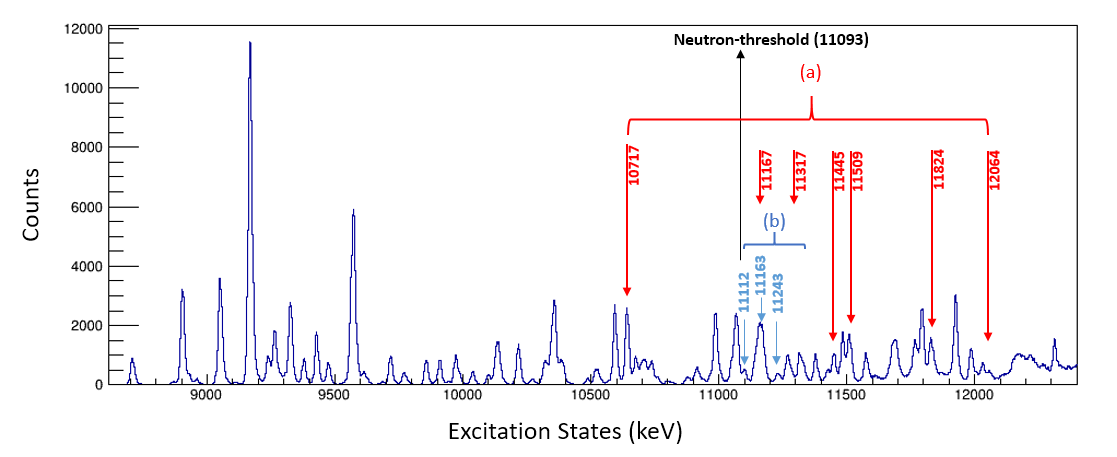
\includegraphics[scale=0.8]{graph/ch5/states2}}
    \caption{Spectrum of $^{26}$Mg in the high-lying states region (excited states above $E_x$ = 8.706 MeV) measured by this work. Energy regions above the $\alpha$ threshold probed by Talwar\citep{Rashi2016} and Massimi\citep{MASSIMI2017} are quoted by red (a) and blue (b) bracket, respectively. The red arrows and values indicate the states that were also observed by Talwar and the blues ones indicate the work by Massimi in units of keV.}
    \label{fig:states2}
    \end{figure}
\end{landscape}

\begin{landscape}
\begin{center}
%\setlength{\LTleft}{0pt} \setlength{\LTright}{0pt}
%\setlength{\tabcolsep}{7mm}
    \begin{longtable}{cc cc cc cc cc}
    %\setlength{\LTleft}{0pt} \setlength{\LTright}{0pt}
    \caption{COMPARISONS WITH STATES of $^{26}$MG POPULATED BY THE (D,P) and (N,$\gamma$) N-TOF REACTIONS \label{tb:dp}\/}\\
    \toprule
    \hline
    \multicolumn{2}{c}{This Work} & \multicolumn{2}{c}{Cujec $et\ al.$\citep{Cujec1964}}  & \multicolumn{2}{c}{Hinds $et\ al.$\citep{Hinds1965}\citep{Hinds1961}}&\multicolumn{2}{c}{Arciszewski $et\ al.$\citep{Arciszewski1984}}& \multicolumn{2}{c}{Massimi $et\ al.$\citep{Massimi}\citep{MASSIMI2017}}       \\
    \multicolumn{2}{c}{($d,p$)}   & \multicolumn{2}{c}{($d,p$)}          & \multicolumn{2}{c}{$(d,p)$}        &  \multicolumn{2}{c}{$(d,p)$}            & \multicolumn{2}{c}{$(n,\gamma)$n-ToF}         \\
      $E_x$(MeV)&    $l_n$        &  $E_x$(MeV)   & $l_n$                & $E_x$(MeV)     &     $l_n$         &  $E_x$(MeV)     &     $l_n$             & $E_x$(MeV)          &    $l_n$              \\
    \midrule
    \endfirsthead % Everything above goes at the top of the 1st page only
% As with the first header, we don't want obscene amounts of space for
% subsequent headings either, and eliminate an em of whitespace.
  \caption[]{{\em Continued}}\\
    \midrule
    \hline
    \multicolumn{2}{c}{This Work} & \multicolumn{2}{c}{Cujec $et\ al.$\citep{Cujec1964}}  & \multicolumn{2}{c}{Hinds $et\ al.$\citep{Hinds1965}\citep{Hinds1961}}&\multicolumn{2}{c}{Arciszewski $et\ al.$\citep{Arciszewski1984}}& \multicolumn{2}{c}{Massimi $et\ al.$\citep{Massimi}\citep{MASSIMI2017}}       \\
    \multicolumn{2}{c}{($d,p$)}   & \multicolumn{2}{c}{($d,p$)}          & \multicolumn{2}{c}{$(d,p)$}        &  \multicolumn{2}{c}{$(d,p)$}            & \multicolumn{2}{c}{$(n,\gamma)$n-ToF}         \\
      $E_x$(MeV)&    $l_n$        &  $E_x$(MeV)   & $l_n$                & $E_x$(MeV)     &     $l_n$         &  $E_x$(MeV)     &     $l_n$             & $E_x$(MeV)          &     $l_n$             \\

    \midrule
    \endhead
    \endfoot % The above section goes at the bottom of continuation pages
  \bottomrule

\endlastfoot


	&		&	0	&		&	0	&	2	&	0	&	2	&		&		\\
1.810(11) 	&		&	1.81	&		&	1.805	&	0+2	&	1.809	&	0,2	&		&		\\
2.940(11) 	&		&	2.94	&		&	2.941	&	0	&	2.938	&	0	&		&		\\
3.583(11) 	&		&	3.58	&	2	&	3.584	&	2	&	3.588	&	2	&		&		\\
3.940(12) 	&		&	3.94	&		&	3.943	&	0	&	3.941	&	0,2	&		&		\\
	&		&	4.32	&		&	4.319	&		&		&		&		&		\\
4.330(11) 	&		&	4.33	&		&	4.331	&		&		&		&		&		\\
4.340(11) 	&		&	4.35	&		&	4.350	&		&		&		&		&		\\
4.831(11) 	&		&	4.83	&	(1,0)	&	4.830	&	0	&	4.834	&	0,2	&		&		\\
4.904(12) 	&		&	4.90	&	2	&	4.896	&	2	&	4.900	&	2	&		&		\\
	&		&	4.97	&		&	4.970	&	2	&		&	2	&		&		\\
5.291(12) 	&		&	5.29	&		&	5.287	&	2	&	5.291	&	2	&		&		\\
5.464(12) 	&		&	5.47	&		&	5.472	&	2	&	5.474	&	2	&		&		\\
5.693(11) 	&		&	5.69	&		&	5.686	&		&		&	0,2	&		&		\\
5.709(12) 	&		&	5.71	&		&	5.710	&		&	5.716	&	0,2	&		&		\\
6.121(12) 	&		&	6.12	&	(0+2)	&	6.120	&	0	&	6.125	&	1	&		&		\\
6.253(12) 	&		&	6.25	&		&	6.253	&		&		&	1,3	&		&		\\
6.617(11) 	&		&	6.62	&	(2+0)	&	6.616	&		&		&	1,3	&		&		\\
6.732(12) 	&		&	6.74	&	(2+0)	&	6.737	&		&	6.744	&	1,3	&		&		\\
6.875(12) 	&		&	6.87	&		&	6.870	&		&	6.878	&	2	&		&		\\
6.967(11) 	&		&	6.97	&		&	6.967	&		&		&	2	&		&		\\
7.058(11) 	&		&	7.06	&		&	7.053	&		&		&	0,2	&		&		\\
7.096(11) 	&		&	7.10	&		&	7.096	&		&		&	3	&		&		\\
7.198(12) 	&		&	7.24	&		&	7.237	&		&	7.262 + 7.282	&		&		&		\\
7.251(10) 	&		&	7.25	&		&	7.251	&		&		&		&		&		\\
7.269(11) 	&		&	7.27	&		&	7.273	&		&		&		&		&		\\
7.347(12) 	&		&	7.34	&		&	7.338	&		&	7.347	&		&		&		\\
	&		&	7.35	&		&	   	&		&		&		&		&		\\
	&		&	7.38	&		&	7.383	&		&		&		&		&		\\
	&		&	7.41	&		&	7.414	&		&		&		&		&		\\
  7.540 (11)  	&		&	7.53	&		&	7.528	&		&	7.543	&		&		&		\\
	&		&	7.67	&		&	7.668	&		&		&		&		&		\\
  7.677 (11)  	&		&	7.68	&		&	   	&		&		&		&		&		\\
  7.712 (12)  	&		&	7.71	&		&	7.714	&		&	7.723	&		&		&		\\
  7.733 (11)  	&		&		&		&		&		&		&		&		&		\\
	&		&	7.76	&		&	7.761	&		&	7.771	&		&		&		\\
  7.809 (11)  	&		&	7.81	&	1	&	7.808	&		&	7.815	&		&		&		\\
	&		&	7.83	&		&	7.842	&		&		&		&		&		\\
  7.942 (10)  	&		&	7.94	&		&	7.945	&		&	7.950	&		&		&		\\
  7.996 (11)  	&		&	8.02	&		&	8.020	&		&		&		&		&		\\
  8.042 (11)  	&		&	8.04	&		&	8.040	&		&		&		&		&		\\
  8.179 (12)  	&		&	8.17	&		&	8.175	&		&		&		&		&		\\
	&		&	(8.19)	&		&	  	&		&		&		&		&		\\
  8.243 (12)  	&		&	8.24	&	0	&	8.243	&		&		&		&		&		\\
  8.393 (11)  	&		&	8.39	&		&	8.388	&		&		&		&		&		\\
  8.454 (10)  	&		&	8.45	&		&	8.451	&		&		&		&		&		\\
  8.497 (11)  	&		&	8.49	&		&	8.494	&		&		&		&		&		\\
  8.527 (11)  	&		&	8.52	&		&	8.524	&		&		&		&		&		\\
	&		&	8.57	&		&	8.565	&		&		&		&		&		\\
  8.621 (11)  	&		&	8.62	&		&	8.617	&		&		&		&		&		\\
	&		&	8.66	&		&		&		&		&		&		&		\\
  8.706 (11)  	&		&	8.69	&		&		&		&		&		&		&		\\
   8.865(11)  	&		&	8.85	&		&		&		&		&		&		&		\\
  8.904 (10)  	&		&	8.89	&		&		&		&		&		&		&		\\
8.931(11)	&		&	8.92	&		&		&		&		&		&		&		\\
  8.960 (11)  	&		&	8.95	&		&		&		&		&		&		&		\\
	&		&	9.03	&	0	&		&		&		&		&		&		\\
   9.052(11)  	&		&	9.05	&		&		&		&		&		&		&		\\
	&		&	9.10	&		&		&		&		&		&		&		\\
  9.167 (11)  	&		&	9.16	&		&		&		&		&		&		&		\\
  9.238 (12)  	&		&	9.22	&		&		&		&		&		&		&		\\
  9.263 (11)  	&		&	9.25	&		&		&		&		&		&		&		\\
   9.322(11)  	&		&	9.30	&		&		&		&		&		&		&		\\
  9.382 (11)  	&		&	9.37	&	0	&		&		&		&		&		&		\\
  9.430 (11)  	&		&	9.42	&	0	&		&		&		&		&		&		\\
  9.476 (11)  	&		&	9.46	&		&		&		&		&		&		&		\\
	&		&	9.53	&		&		&		&		&		&		&		\\
   9.578(11)  	&		&	9.56	&		&		&		&		&		&		&		\\
   9.613(11)  	&		&	9.62	&		&		&		&		&		&		&		\\
  9.683 (10)  	&		&	9.67	&		&		&		&		&		&		&		\\
  9.716 (11)  	&		&	9.71	&		&		&		&		&		&		&		\\
  9.770 (11)  	&		&	9.76	&		&		&		&		&		&		&		\\
	&		&	9.81	&		&		&		&		&		&		&		\\
  9.856 (11)  	&		&	9.84	&		&		&		&		&		&		&		\\
  9.991 (11)  	&		&	9.90	&		&		&		&		&		&		&		\\
  9.985 (11)  	&		&	9.93	&		&		&		&		&		&		&		\\
	&		&	9.97	&		&		&		&		&		&		&		\\
  10.040(10)  	&		&	10.03	&		&		&		&		&		&		&		\\
  10.100(10)  	&		&	10.09	&		&		&		&		&		&		&		\\
  10.137(11)  	&		&	10.12	&		&		&		&		&		&		&		\\
	&		&	10.21	&		&		&		&		&		&		&		\\
  10.269(11)  	&		&	10.27	&		&		&		&		&		&		&		\\
  10.320(11)  	&		&	10.32	&		&		&		&		&		&		&		\\
  10.355(12)  	&		&	10.36	&		&		&		&		&		&		&		\\
  10.385(12)  	&		&	10.40	&		&		&		&		&		&		&		\\
	&		&	10.42	&		&		&		&		&		&		&		\\
  10.487(12)  	&		&	10.48	&		&		&		&		&		&		&		\\
  10.522(11)  	&		&	10.52	&		&		&		&		&		&		&		\\
10.568(11)	&		&		&		&		&		&		&		&		&		\\
  10.595(11)  	&		&	10.59	&		&		&		&		&		&		&		\\
     10.641(11) 	&		&	10.64	&		&		&		&		&		&		&		\\
     10.676(11) 	&		&		&		&		&		&		&		&		&		\\
     10.708(10) 	&	1	&	10.70	&		&		&		&		&		&		&		\\
     10.735(11) 	&	2	&		&		&		&		&		&		&		&		\\
     10.808(10) 	&	2	&		&		&		&		&		&		&		&		\\
     10.875(11) 	&	3	&		&		&		&		&		&		&		&		\\
     10.915(10) 	&	2	&	10.91	&		&		&		&		&		&		&		\\
   10.988(11)   	&	3	&	10.98	&		&		&		&		&		&		&		\\
	&		&	11.00	&		&		&		&		&		&		&		\\
    11.069(10)  	&	2	&	11.07	&		&		&		&		&		&		&		\\
     11.112(11) 	&	3	&	11.12	&		&		&		&		&		&	11.112	&	0	\\
	&		&		&		&		&		&		&		&	11.154	&	1	\\
	&		&		&		&		&		&		&		&	11.163	&	0	\\
    11.165(10)  	&	1	&	11.16	&		&		&		&		&		&	11.169	&	(0)	\\
	&		&		&		&		&		&		&		&	11.171	&	0	\\
	&		&		&		&		&		&		&		&	11.183	&	1	\\
	&		&	11.22	&		&		&		&		&		&	11.190	&	0	\\
    11.232(10)  	&	2	&		&		&		&		&		&		&	11.243	&	(1)	\\
    11.267(10)  	&	2	&		&		&		&		&		&		&	11.274	&	0	\\
	&		&	11.28	&		&		&		&		&		&	11.280	&	(1	\\
	&		&		&		&		&		&		&		&	11.285	&	1	\\
	&		&		&		&		&		&		&		&	11.289	&	(1)	\\
	&		&		&		&		&		&		&		&	11.295	&	(1)	\\
    11.317(11)  	&	3	&	11.31	&		&		&		&		&		&	11.328	&	1	\\
	&		&	11.34	&		&		&		&		&		&	11.344	&	(1)	\\									
    11.374(12)  	&	3	&	11.38	&		&		&		&		&		&	11.362	&	(0)	\\
    11.425(12)  	&	2	&		&		&		&		&		&		&				\\
	&		&		&		&		&		&		&		&	11.393	&	(2)	\\
	&		&		&		&		&		&		&		&		&		\\
    11.447(11)  	&	3	&	11.45	&		&		&		&		&		&	11.441	&	2	\\
	&		&		&		&		&		&		&		&	11.466	&	(3)	\\
    11.482(10)  	&	1	&	11.48	&		&		&		&		&		&		&		\\
    11.509(10)  	&	3	&	11.51	&		&		&		&		&		&	11.500	&	1	\\
	&		&		&		&		&		&		&		&	11.527	&	(1)	\\
     11.573(11) 	&	3	&	11.57	&		&		&		&		&		&		&		\\
	&		&		&		&		&		&		&		&	11.592	&	(1)	\\
     11.613(11) 	&	2	&	11.60	&		&		&		&		&		&	11.613	&	(1)	\\
   11.690(10)   	&	1	&	11.69	&		&		&		&		&		&		&		\\
   11.767(11)   	&	3	&	11.76	&		&		&		&		&		&		&		\\
   11.790(11)   	&	2	&	11.79	&		&		&		&		&		&		&		\\
   11.828(10)   	&	3	&	11.83	&		&		&		&		&		&		&		\\
     11.874(11) 	&	2	&	11.90	&		&		&		&		&		&		&		\\
    11.927(11)  	&	3	&		&		&		&		&		&		&		&		\\
    11.981(11)  	&	2	&		&		&		&		&		&		&		&		\\
     12.032(11) 	&	1	&	12.00	&		&		&		&		&		&		&		\\
     12.059(12) 	&	3	&		&		&		&		&		&		&		&		\\
    12.311(11)  	&	1	&		&		&		&		&		&		&		&		\\
	&		&	12.50	&		&		&		&		&		&		&		\\
	&		&	12.57	&		&		&		&		&		&		&		\\

    \end{longtable}
\end{center}
\end{landscape}



\subsection{Comparison with the reactions $^{23}$Na($\alpha$,p$\gamma$)$^{26}$Mg and $^{12}$C($^{18}$O,$\alpha$)$^{26}$Mg}
In addition to the reactions mentioned above, more methods have been used to explore the high-spin states ($J>4$) in $^{26}$Mg, including the proton-$\gamma$-ray coincidence measurements in the $^{23}$Na($\alpha$,p$\gamma$)$^{26}$Mg (Glatz $et\ al.$\citep{Glatz1986}) and the heavy-ion reactions by $^{12}$C($^{18}$O,$\alpha$)$^{26}$Mg (Gustafson $et\ al.$ \citep{Gustafson1976}), as listed in Table~\ref{tb:other}. Though both reactions are dependable ways of investigating high-spin states, the spin-parity assignments obtained in these works showed limited agreement, possibly due to the fact that \citep{Glatz1986} used the particle-$\gamma$-ray angular correlation method while \citep{Gustafson1976} predicted them by Hauser-Feshbach (HF) calculation.

The neutron-transfer reaction performed in this work can only give the possible $l_n$ values. The $J^{\pi}$ values associated with   $l_n$s are  $J^{\pi}=2^+$ for $l_n=$0;
$J^{\pi}=1^-,3^-$ for $l_n=$1;
$J^{\pi}=0^+,2^+,4^+$ for $l_n=$2;
$J^{\pi}=1^-,3^-,5^-$ for $l_n=$3, etc., which does not provide sufficient information for high-spin(-parity) assignments except  states with $l_n=$3 , for example, $E_x=$11.537(11) MeV and 11.767(11) MeV potentially agree with \citep{Gustafson1976}'s calculation.



\begin{center}
%\setlength{\LTleft}{0pt} \setlength{\LTright}{0pt}
%\setlength{\tabcolsep}{7mm}
    \begin{longtable}{cc cc cc}
    %\setlength{\LTleft}{0pt} \setlength{\LTright}{0pt}
    \caption{COMPARISONS WITH STATES of $^{26}$MG POPULATED BY OTHER REACTIONS \label{tb:other}\/}\\
    \toprule
    \hline
     \multicolumn{2}{c}{This Work} & \multicolumn{2}{c}{Glatz $et\ al.$\citep{Glatz1986}}         &\multicolumn{2}{c}{Gustafson $et\ al.$ \citep{Gustafson1976}}  \\
     \multicolumn{2}{c}{($d,p$)}   & \multicolumn{2}{c}{ ($\alpha,p\gamma$) }                     & \multicolumn{2}{c}{($^{18}O,\alpha$)}                         \\
       $E_x$(MeV)&    $l_n$        &  $E_x$(MeV)   & $J^{\pi}$                                    & $E_x$(MeV)         &           $J^{\pi}$                      \\
    \midrule
    \endfirsthead % Everything above goes at the top of the 1st page only
% As with the first header, we don't want obscene amounts of space for
% subsequent headings either, and eliminate an em of whitespace.
  \caption[]{{\em Continued}}\\
    \midrule
    \hline
     \multicolumn{2}{c}{This Work} & \multicolumn{2}{c}{Glatz $et\ al.$\citep{Glatz1986}}         &\multicolumn{2}{c}{Gustafson $et\ al.$ \citep{Gustafson1976}}  \\
     \multicolumn{2}{c}{($d,p$)}   & \multicolumn{2}{c}{ ($\alpha,p\gamma$) }                     & \multicolumn{2}{c}{($^{18}O,\alpha$)}                         \\
       $E_x$(MeV)&    $l_n$        &  $E_x$(MeV)   & $J^{\pi}$                                    & $E_x$(MeV)         &           $J^{\pi}$                      \\

    \midrule
    \endhead
    \endfoot % The above section goes at the bottom of continuation pages
  \bottomrule

\endlastfoot

  &   & 0.000 & 0 & 0 &   \\
1.810(11)   &   & 1.809 & 2 & 1.83  & (2$^+$)                 \\
2.940(11)   &   & 2.938 & 2 & 2.96  & (2$^+$)                 \\
3.583(11)   &   & 3.588 & 0 & 3.58  &                         \\
3.940(12)   &   & 3.941 & 3 & 3.96  & (3$^+$),(4$^-$)         \\
  &   & 4.318 & 4 &   &   \\
4.330(11)   &   & 4.332 & 2 & 4.32  & (2$^+$),(3$^+$)         \\
4.340(11)   &   & 4.350 & 3 &   &                         \\
4.831(11)   &   & 4.835 & 2 & 4.82  & (2$^+$)                 \\
4.904(12)   &   & 4.901 & 4 & 4.90  & (4$^+$)                 \\
  &   & 4.972 & 0 & 5.00  &                         \\
5.291(12)   &   & 5.292 & 2 & 5.31  & (2$^+$)                 \\
5.464(12)   &   & 5.475 & 4 & 5.48  & (4$^+$)                 \\
5.693(11)   &   & 5.692 & 1 & 5.68  & (1$^-$)                 \\
5.709(12)   &   & 5.715 & 4 & 5.73  & (3$^+$)                 \\
6.121(12)   &   & 6.125 & 3 & 6.17  & (2$^+$)                 \\
6.253(12)   &   & 6.256 & 0 & 6.30  & ((1$^-$, 2$^-$))        \\
6.617(11)   &   & 6.623 & 4$^+$ & 6.60  & (2$^+$)                 \\
  &   & 6.634 & 1 &   &   \\
6.732(12)   &   & 6.745 & 2 & 6.71  & (3$^-$)                 \\
6.875(12)   &   &   &   & 6.87  & ((2$^+$, 3$^+$))        \\
6.967(11)   &   & 6.978 & 5$^+$   & 6.94  & ((2$^+$, 3$^+$))        \\
7.058(11)   &   &   &   & 7.08  & (2$^+$)                 \\
7.096(11)   &   &   &   &   &   \\
7.198(12)   &   &   &   &   &   \\
7.251(10)   &   & 7.242 & 3 &   &   \\
7.269(11)   &   & 7.283 & 4$^-$ &   &   \\
7.347(12)   &   &   &   & 7.34  & ((2$^+$, 3$^+$))          \\
  &   & 7.395 & 5$^+$ & 7.42  & ((2$^+$, 3$^+$))          \\
  7.540 (11)    &   &   &   & 7.54  & ((4$^+$, 5$^+$))          \\
  7.677 (11)    &   & 7.677 & 3$^-$,4$^-$,5$^-$ & 7.64  & ((2$^+$, 3$^+$, 4$^-$))   \\
  7.712 (12)    &   &   &   & 7.72  &                           \\
  7.733 (11)    &   & 7.773 & 4 &   & ((2$^+$, 3$^+$))          \\
  7.809 (11)    &   &   &   &   &                           \\
  7.942 (10)    &   & 7.953 & 5$^-$ & 7.96  & (4$^+$)                   \\
  7.996 (11)    &   &   &   &   &                           \\
  8.042 (11)    &   &   &   & 8.07  & (4$^+$)                   \\
  8.179 (12)    &   & 8.202 & 6$^+$ & 8.16  & (3$^-$)                   \\
  8.243 (12)    &   &   &   &   &                           \\
  8.393 (11)    &   &   &   & 8.38  & (6$^+$)                   \\
  8.454 (10)    &   &   &   &   &                           \\
  8.497 (11)    &   & 8.472 & 6$^+$ & 8.50  & (6$^+$)                   \\
  8.527 (11)    &   &   &   &   &                           \\
  8.621 (11)    &   & 8.624 & 3,4,5 &   &                           \\
  8.706 (11)    &   & 8.670 & 3,5 & 8.70  & (5$^-$)                   \\
   8.865(11)    &   &   &   & 8.84  & (4$^+$)                   \\
  8.904 (10)    &   & 9.065 & 5 & 8.91  & (6$^+$)                   \\
8.931(11) &   &   &   &   &                           \\
  8.960 (11)    &   &   &   & 9.85  & ((2$^+$, 3$^+$))          \\
   9.052(11)    &   &   &   & 9.05  & ((4$^-$))                 \\
  9.167 (11)    &   & 9.112 & 6$^+$ & 9.13  & ((5$^-$,6$^-$))           \\
  9.238 (12)    &   & 9.169 & 6$^-$ & 9.22  & ((2$^+$,3$^+$))           \\
  9.263 (11)    &   &   &   &   &                           \\
   9.322(11)    &   &   &   & 9.30  & ((5$^-$, 6$^-$))          \\
  9.382 (11)    &   & 9.383 & 6$^+$ &   &   \\
  9.430 (11)    &   &   &   &   &   \\
  9.476 (11)    &   &   &   &   &   \\
  &   & 9.542 & 5 & 9.53  & ((5$^-$, 6$^-$))        \\
   9.578(11)    &   &   &   & 9.57  & (7$^-$)                 \\
   9.613(11)    &   &   &   &   &                         \\
  9.683 (10)    &   &   &   &   &                         \\
  9.716 (11)    &   &   &   &   &                         \\
  9.770 (11)    &   &   &   &   &                         \\
  9.856 (11)    &   & 9.829 & 7$^+$ & 9.84  & ((5$^-$, 7$^+$))        \\
  9.991 (11)    &   &   &             & 9.91  & ((2$^+$, 3$^+$))        \\
  9.985 (11)    &   & 9.989 & 6$^+ $      & 9.95  & (4$^-$)                 \\
  10.040(10)    &   &   &   & 10.02 & (3$^-$)                 \\
  10.100(10)    &   &   &   & 10.06 & ((3$^-$, 4$^-$))        \\
  10.137(11)    &   &   &   &   &                         \\
  &   &   &   & 10.16 & ((5$^-$, 7$^+$))        \\
  10.269(11)    &   &   &   &   &                         \\
  10.320(11)    &   &   &   &   &                         \\
  10.355(12)    &   &   &   &   &                         \\
  10.385(12)    &   &   &   &   &                         \\
  &   &   &   & 10.42 & ((3$^-$,5$^+$))         \\
  10.487(12)    &   &   &   & 10.48 & (6$^+$)                 \\
  10.522(11)    &   &   &   & 10.52 & (2$^+$)                 \\
10.568(11)  &   &   &   &   &                         \\
  10.595(11)    &   &   &   &   &                         \\
     10.641(11)   &   &   &   &   &                         \\
     10.676(11)   &   &   &   & 10.66 & ((4$^+$, 5$^+$))        \\
     10.708(10)   & 1 &   &   &   &                         \\
     10.735(11)   & 2 &   &   & 10.74 & (7$^-$)                 \\
     10.808(10)   & 2 &   &   &   &   \\
     10.875(11)   & 3 &   &   &   &   \\
     10.915(10)   & 2 &   &   &   &   \\
   10.988(11)     & 3 &   &   & 10.96 & (7$^-$)                   \\
    11.069(10)    & 2 &   &   & 11.08 & ((4$^+$, 6$^-$))          \\
     11.112(11)   & 3 &   &   &   &                           \\
    11.165(10)    & 1 &   &   & 11.16 & ((6$^+$, 8$^-$))          \\
    11.232(10)    & 2 &   &   &   &                           \\
    11.267(10)    & 2 &   &   &   &                           \\
    11.317(11)    & 3 &   &   & 11.31 & (7$^-$)                   \\
    11.374(12)    & 3 & 11.392  & 7 &   &                           \\
    11.425(12)    & 2 &   &   & 11.42 & ((5$^-$, 7$^+$))          \\
    11.447(11)    & 3 &   &   & 11.45  & ((5$^-$, 7$^+$))            \\
    11.482(10)    & 1 &   &   &   &                           \\
    11.509(10)    & 3 &   &   & 11.51 & ((4$^+$, 6$^-$))          \\
     11.573(11)   & 3 & 11.570  & 7 & 11.56 & ((5$^-$, 6$^-$))          \\
     11.613(11)   & 2 &   &   &   &                           \\
  &   &   &   & 11.64 & (8$^+$)                   \\
   11.690(10)     & 1 &   &   &   &                           \\
   11.767(11)     & 3 &   &   & 11.77 & ((5$^-$, 7$^+$))          \\
   11.790(11)     & 2 &   &   &   &                           \\
  &   &   &   &   &                           \\
   11.828(10)     & 3 &   &   & 11.83 & (6$^+$)                   \\
     11.874(11)   & 2 &   &   &   &                           \\
    11.927(11)    & 3 &   &   & 11.94 & ((6$^+$, 8$^-$))          \\
    11.981(11)    & 2 &   &   &   &                           \\
     12.032(11)   & 1 &   &   & 12.03 & ((7$^-$, 9$^+$))          \\
     12.059(12)   & 3 &   &   &   &                           \\
  &   &   &   & 12.10 & ((6$^+$, 8$^-$))          \\
  &   &   &   & 12.14 & ((6$^+$, 8$^-$))          \\
  &   &   &   & 12.20 & ((6$^+$, 9$^+$))          \\
  &   &   &   & 12.28 & ((4$^+$, 5$^+$, 6$^-$))   \\
    12.311(11)    & 1 &   &   & 12.34 & ((5$^-$, 7$^+$))          \\
  &   &   &   & 12.40 & ((6$^+$, 8$^-$))          \\
  &   & 12.479  & 8$^-$,7$^+$ & 12.45 & (6$^+$)                   \\
  &   &   &   & 12.53 & (8$^+$)                   \\
  &   &   &   & 12.63 & ((6$^+$, 8$^+$))          \\
  &   &   &   & 12.88 & ((6$^+$, 8$^-$))          \\
  &   &   &   & 12.95 & ((7$^-$, 9$^+$))          \\
  &   &   &   & 13.00 & ((6$^+$, 9$^+$))          \\
  &   &   &   & 13.06 & ((6$^+$, 9$^+$))          \\
  &   &   &   & 13.12 & (7$^-$)                   \\
  &   &   &   & 13.19 & (8$^+$)                   \\
  &   &   &   & 13.25 & ((7$^-$, 9$^+$))          \\
  &   &   &   & 13.35 & ((6$^+$, 7$^-$, 9$^+$))   \\
  &   &   &   & 13.39 & (9$^+$)                   \\
  &   &   &   & 13.46 & ((6$^+$, 8$^-$))          \\
  &   &   &   & 13.52 & (9$^+$)                   \\
  &   &   &   & 13.59 & (8$^+$)                   \\
  &   &   &   & 13.64 & (9$^-$)                   \\
  &   &   &   & 13.69 & ((6$^+$, 8$^-$))          \\
  &   &   &   & 13.75 & ((6$^+$, 8$^-$))          \\
  &   &   &   & 13.85 & (8$^+$)                   \\
  &   &   &   & 13.90 & ((7$^-$, 8$^+$))          \\
  &   &   &   & 13.955  & (7$^-$)                   \\
  &   &   &   & 14.08 &   (9$^-$)                 \\
  &   &   &   & 14.14 &   ((9$^-$, 10$^+$))       \\
  &   &   &   & 14.21 &   (9$^-$)                 \\
  &   &   &   & 14.30 &   (8$^+$)                 \\
  &   &   &   & 14.38 &   (7$^-$)                 \\
  &   &   &   & 14.50 &   (8$^+$)                 \\
  &   &   &   & 14.56 &   ((7$^-$, 9$^+$))        \\
  &   &   &   & 14.62 &   (6$^+$)                 \\
  &   &   &   & 14.66 &   ((6$^+$, 8$^-$))        \\
  &   &   &   & 14.70 &   ((7$^-$, 8$^+$))        \\
  &   &   &   & 14.75 &   ((8$^+$,9$^-$))         \\
  &   &   &   & 14.86 &   (8$^+$)                 \\
  &   &   &   & 14.92 &   (8$^+$)                 \\
  &   &   &   & 14.96 &   (8$^+$)                 \\
  &   &   &   & 15.00 &   (8$^+$)                 \\
  &   &   &   & 15.14 &   (8$^+$)                 \\
  &   &   &   & 15.21 &   ((8$^+$, 9$^-$))        \\
  &   &   &   & 15.35 &   (8$^+$)                 \\
  &   &   &   & 15.4  &   (9$^-$)                 \\
  &   &   &   & 15.46 &   ((9$^-$, 10$^+$))       \\
  &   &   &   & 15.56 &   (8$^+$)                 \\
  &   &   &   & 15.70 &   ((9$^-$, 10$^+$))       \\
  &   &   &   & 15.77 &   (8$^+$)                 \\
  &   &   &   & 15.84 &   (9$^-$)                 \\
  &   &   &   & 15.91 &   ((8$^+$, 9$^-$))        \\
  &   &   &   & 15.98 &   (7$^+$)                 \\
  &   &   &   & 16.04 &   (7$^-$)                 \\
  &   &   &   & 16.10 &   (7$^-$)                 \\
  &   &   &   & 16.20 &   (8$^+$)                 \\
  &   &   &   & 16.26 &   (9$^-$)                 \\
  &   &   &   & 16.35 &   ((8$^+$, 9$^-$))        \\

    \end{longtable}
\end{center}




\section{Angular Distribution Analysis}
As mentioned in Chapter 4, the Grand Raiden spectrometer was operated in 3 angle modes including the 0$^{\circ}$ mode, so that measurements can be taken in the angular range from 0.5$^{\circ}$ to about 45$^{\circ}$ of the high-lying states (the 3rd setting B3). The measurements of the angular distributions will help to determine the orbital momentum of the transferred neutron by comparing the experimental data with   Distorted Wave Born Approximation (DWBA) calculations. In this work, the DWUCK4 code~\citep{DWUCK4} was used for the DWBA calculations since it based on the zero range correction and provided the well-studied fitting parameters for the (d,p) reaction ~\citep{DWUCK4}.

\begin{center}
  \begin{longtable}{lcccccccccccc}
    \caption{OPTICAL POTENTIAL  PARAMETERS  USED IN THE DWBA ANALYSIS OF $^{25}$Mg(d,p)$^{26}$Mg ~\citep{HATANAKA1984530} \label{tbl:opticalpotential}\/}\\
        \toprule
        \toprule
         Target  &  & $V_0$   & $r_0$  & $a_0$   &  $W_v$  & $W_D$  & $r_W$ & $a_W$  & $V_{LS}$  & $r_{LS}$ & $a_{LS}$ & $r_c$  \\
         nucleus &  &  MeV  &  fm  & fm    &   MeV & MeV  & fm  & fm   &  MeV    &   fm   &   fm   & fm \\
        \midrule
\endfirsthead

\endhead % Everything above here (and below the \endfirsthead) goes at the top
         % of continuation pages.  The [] argument prevents a duplicate
         % entry from appearing in the table of contents.
% The following 3 lines are provided as an example only -- per ND
% guidelines, the footer at the bottom of a page for a longtable
% should not have a bottom line.  Only the absolute bottom of the
% table should have a final \bottomline

%  \midline
%  \multicolumn{6}{|r|}{\textit{continued}\ldots} \\
%  \bottomrule
\endfoot % The above section goes at the bottom of continuation pages
  \bottomrule
\endlastfoot % The very last bottom of the table
   $^{25}$Mg    &d & 74.05   &  1.17  &   0.804 &   3.81  &  9.90  & 1.325 &  0.731 &   3.51  &   1.07 &  0.66  & 1.3  \\
                &p & 37.57   &  1.144 &   0.69  &   9.88  &  0.0   & 1.32  &  0.657 &   5.6   &   1.01 &  0.6   & 1.25 \\
  \end{longtable}
\end{center}

The optical potential parameters used in the DWBA analysis of $^{25}$Mg(d,p)$^{26}$Mg is listed in Table~\ref{tbl:opticalpotential}. This set of parameters is first applied to the low energy $^{13}$C data measured in this experiment and compared with Hatanaka's measurement~\citep{HATANAKA1984530} in order to verify the reproducibility. As shown in Fig.~\ref{fig:13C}, the DWBA calculation in this experiment is consistent with Hatanaka's work, which proves that the optical potential parameters provided by Hatanaka should also work in our calculations.



\begin{landscape}
\begin{figure}[tpb]
  \begin{center}
    \centerline{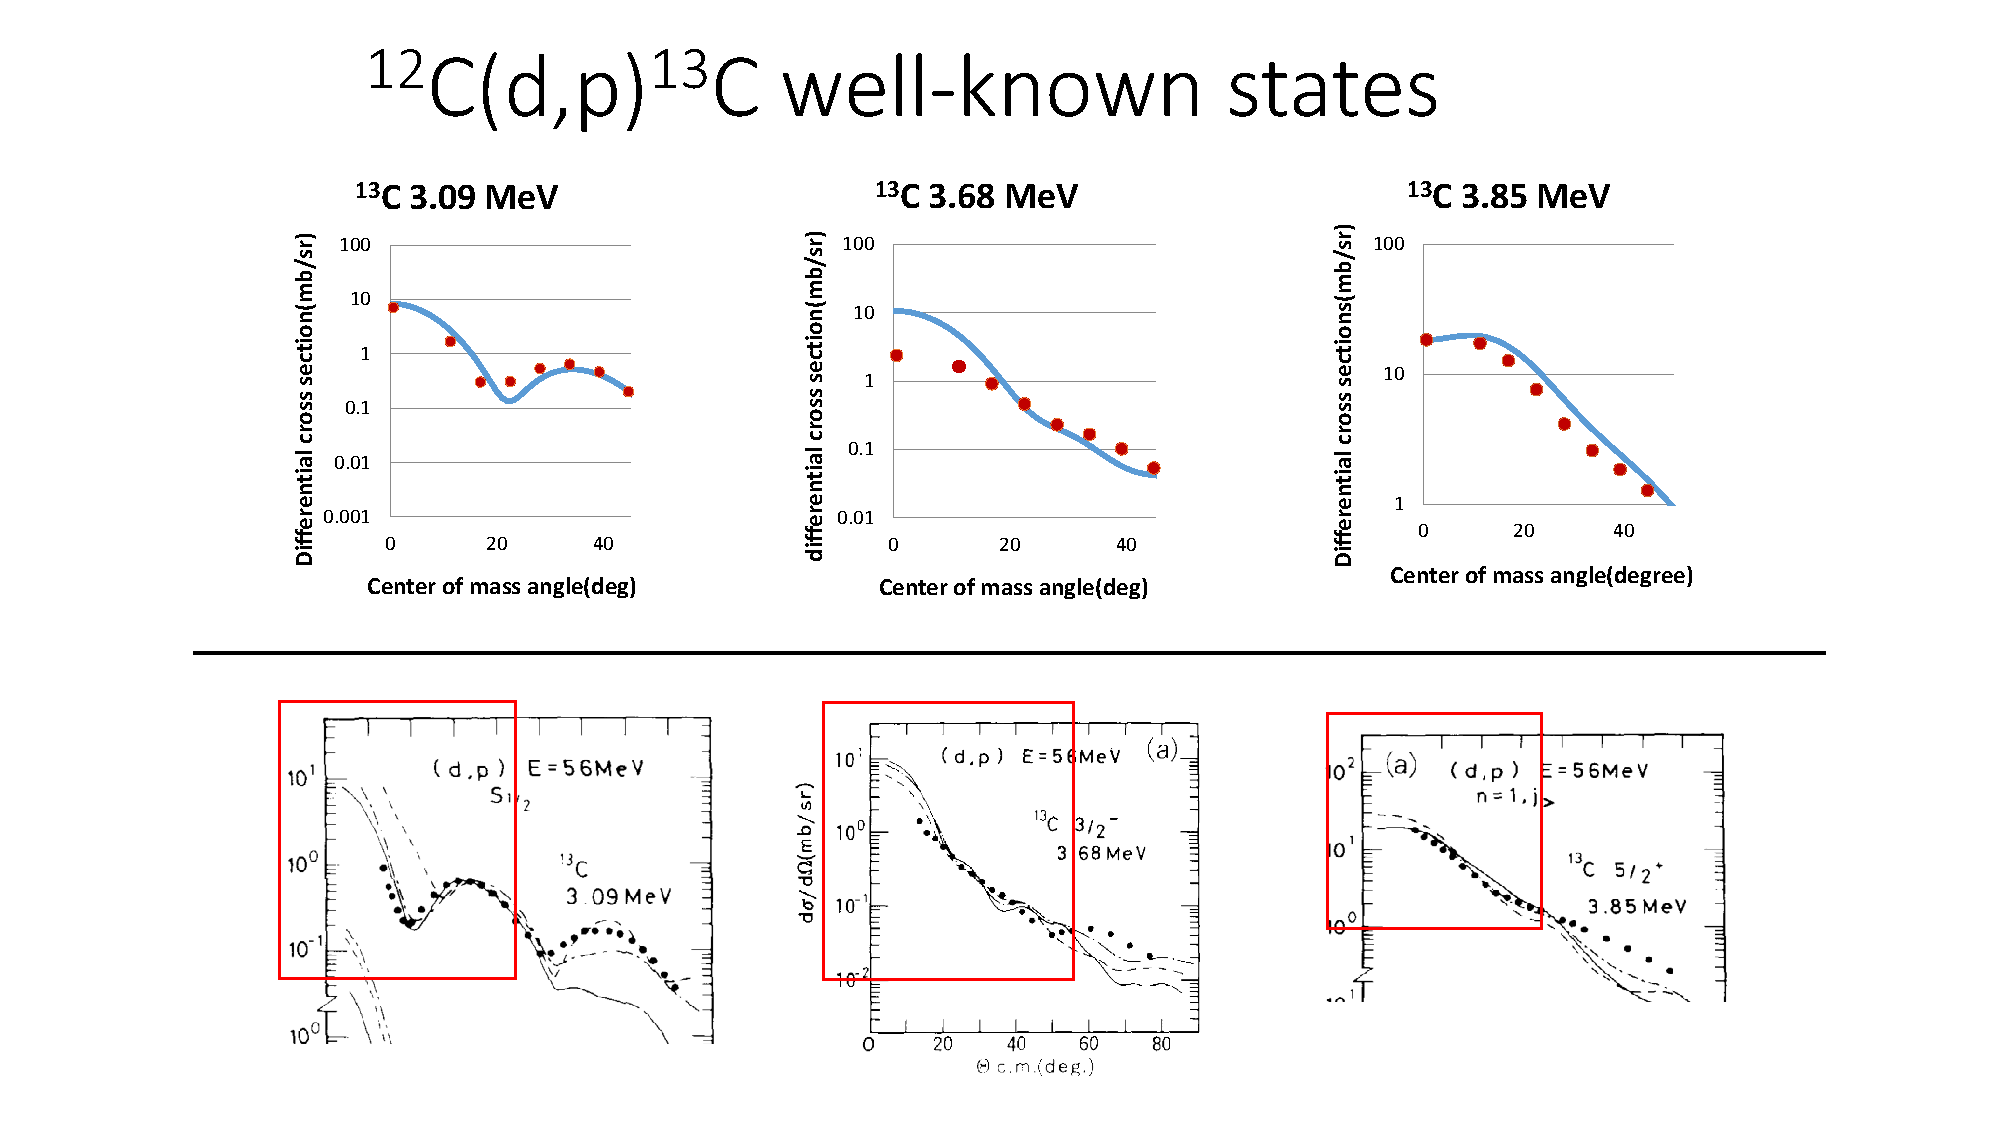
\includegraphics[scale=0.6]{graph/ch5/13C}}
    \caption{Top panel: Angular distributions using DWUCK4 for excited states obtained from the work ( The $^{12}$C(d,p)$^{13}C$ reaction at 56 MeV). Bottom panel: The comparison with results from \citep{HATANAKA1984530} using the same set of optical potential parameters.  }
    \label{fig:13C}
  \end{center}
\end{figure}
\end{landscape}

\begin{landscape}
    \begin{figure}[tpb]
    \centerline{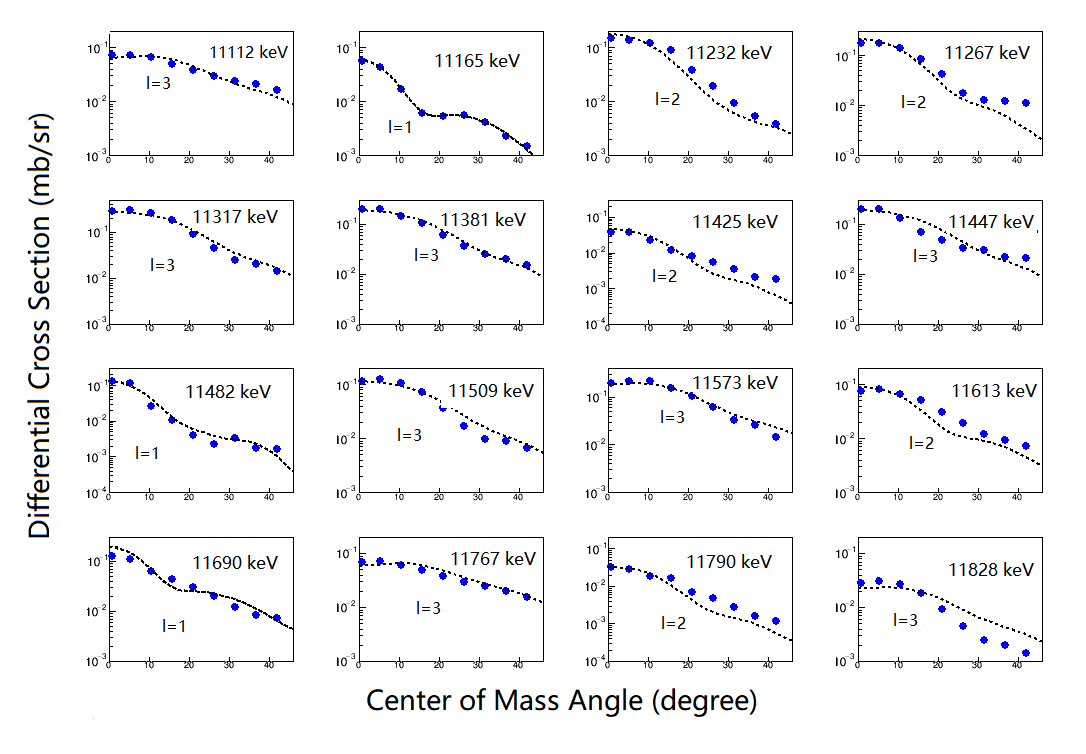
\includegraphics[scale=0.7]{graph/ch5/dwba}}
    \caption{Angular distributions using DWUCK4 for excited states above the neutron threshold obtained from $^{25}$Mg(d,p)$^{26}$Mg reaction at 56 MeV, where $l_n$ is the orbital momentum of the transferred neutron. }
    \label{fig:26Mg}
    \end{figure}
\end{landscape}


The DWBA calculations are then  performed for the high-lying states from 8.706 MeV to  12.311 MeV for the measured angular distributions. The  angular distributions and the DWBA calculations are shown in Fig.~\ref{fig:26Mg}. The possible orbital momenta of the transferred neutron of these states are listed in Tables in the last section.

In the low energy region , there is no measurement for the spin orbital assignment. However, Cujec and Hinds  performed the DWBA calculation  and assignment the J$^{\pi}$ value for some states as listed in Table~\ref{tb:dp}.
Hinds showed some angular distributions and the large cross sections at backward angles are clear indications for   contributions from Compound Nucleus reactions. Cujac only measured two angles but the list of states extends into the $\alpha$-unbound range but has large energy errors. DWBA  calculations are not really appropriate at low energies, nevertheless Hinds fits some
$l_n$-values to the forward angles. In general, these low-lying states are strongly populated in this work, the same as those populated in works of Hinds and Cujec  by either (d,p) reaction and (t,p) reaction.
In the astrophysically important excitation energy region the  level density is high in $^{26}$Mg  above the alpha threshold. For the (d,p) reaction the relative neutron  spectroscopic factors $S_n(rel)$ are extracted from transfer reactions by a comparison of experimental cross sections and the result of DWBA calculations by
\begin{equation}
    \label{eq:S_n}
    \begin{aligned}
\frac{d\sigma_{exp}}{d\Omega} = S_n(rel) N \sigma_{DWBA}
        \end{aligned}
\end{equation}
where N refers to the normalization constant i.e. N = 1.55 for (d,p) reactions~\citep{DWUCK4}.

The neutron widths $\Gamma_{n}$ of unbound states are correlated to the spectroscopic factors $S_n(rel)$ by~\citep{SCHIFFER1963246}:
\begin{equation}
    \label{eq:width_n}
    \begin{aligned}
\Gamma_{n} &=  S_n(rel)\times \Gamma_{sp}
        \end{aligned}
\end{equation}
where $\Gamma_{sp}$ is the calculated neutron single-particle width using the optical potential parameters listed in Table~\ref{tbl:opticalpotential} by DWUCK4.
The resulting resonance parameters for the resonances contributed to the region of interests have  been listed in Table~\ref{tb:reaction_parameters} along with the corresponding reaction rates in this (d,p) measurements.

\begin{landscape}
\setlength{\capwidth}{0.7\textwidth}

    \begin{table}[tpb]
        \begin{centering}
        \caption{ The $^{26}$Mg resonance parameters and the corresponding excitation energies above the neutron-threshold observed in the present work. }
        \label{tb:reaction_parameters}
    \begin{tabular}{c c c c c c c c }
    \toprule
    \toprule
    E$_x$   &       E$_R^{c.m.}$&   l$_n$    &   $\Gamma_{sp}$   &   (2J+1)$S_n$ &  (2J+1)$\Gamma_n$    &  $\Gamma_\gamma$ & $\omega\gamma_{(\alpha,\gamma)}$    \\
    keV     &       keV         &   $\hbar$  &   eV              &               &  eV                  &   eV        &          eV       \\
 \hline


        \hline
     \end{tabular}
      \end{centering}
    \end{table}

\end{landscape}

%\section{Discussion}


% % uncomment the following lines,
% if using chapter-wise bibliography
%
% \bibliographystyle{ndnatbib}
% \bibliography{example}



%
%
% Chapter Six
%

\chapter{REACTION RATES AND IMPLICATIONS}
\section{Reaction Rates Calculation}
As discussed in Chapter 1, the reaction rate for the narrow resonances is given by
 \begin{equation}
 \label{eq:rate_1}
    \begin{aligned}
         N_A<\sigma v> =( \frac{2 \pi}{\mu k T_9 })^{3/2}h_2 \sum_i(\omega \gamma)_i exp(\frac{-E_{R,i}}{kT_9})
        \end{aligned}
\end{equation}
in units of cm$^3$ s$^{-1}$ mole$^{-1}$, and
 \begin{equation}
 \label{eq:rate_2}
    \begin{aligned}
         N_A<\sigma v> = 1.54 \times 10^{5} (\mu T_9)^{-3/2} \sum_i (\omega \gamma)_i \frac{-11.605E_{R,i}}{T_9}
        \end{aligned}
\end{equation}
in units of cm$^3$ s$^{-1}$ mole$^{-1}$ if applying the numerical values to the equation above, where $\mu$ refers to the reduced mass, $T_9$ the astrophysical temperature in in units of GK, $ (\omega \gamma)_i$ the resonance strength in the i$^{th}$ resonance in eV, $E_{R,i}$ the resonance energy of the  i$^{th}$ resonance in the center of mass system in MeV, respectively.

To calculate the reaction rate from Eq.\ref{eq:rate_2}, $T_9$ is associated with the effective temperature that  enables the stellar  burning, $E_{R,i}$  is determined by
 \begin{equation}
 \label{eq:Er}
    \begin{aligned}
    E_{R,i} = E_{x,i} - Q
        \end{aligned}
\end{equation}
where E$_{x,i}$ is the excitation energy of the i$_{th}$ excited states of the compound nuclei and Q is the Q-value of the reaction, i.e. Q = 10.615 MeV in the $^{22}$Ne($\alpha,\gamma$)$^{26}$Mg reaction in this work.
The resonance strength  $(\omega \gamma)_i$ is given by
 \begin{equation}
    \label{eq:strength}
    \begin{aligned}
    \omega \gamma_{i} = \frac{2J_{res} + 1}{(2J_1 + 1)(2J_2 + 1)} \frac{\Gamma_{in} \Gamma_{out}}{\Gamma_{tot}}
        \end{aligned}
\end{equation}
where $J_{res}$, $J_1$, $J_2$ refer to the spins of the resonance, the target nuclei $^{22}$Ne (J = 0) and the incoming $\alpha$ particle (J = 0), respectively. The particle widths  $\Gamma$ can be written as $\Gamma_{tot} = \Gamma_\alpha + \Gamma_\gamma$ for neutron bound states and  $\Gamma_{tot} = \Gamma_\alpha + \Gamma_\gamma + \Gamma_n$ for neutron unbound states.

As a result, Eq.\ref{eq:strength} becomes
 \begin{equation}
    \label{eq:width_n_bound}
    \begin{aligned}
 \omega \gamma_{(\alpha,\gamma)} &= (2J_{res} + 1) \frac{\Gamma_\alpha \Gamma_\gamma }{\Gamma_\alpha + \Gamma_\gamma } \\
                                & \sim (2J_{res} + 1)\Gamma_\alpha
        \end{aligned}
\end{equation}
for neutron bound states. Because of the large Coulomb barrier for $\alpha$ particles that the approximation $\Gamma_\alpha \ll \Gamma_\gamma , \Gamma_n$ has been made for low energy resonances.


Similarly, we obtain neutron unbound states,
\begin{equation}
    \label{eq:width_n_unbound1}
    \begin{aligned}
 \omega \gamma_{(\alpha,\gamma)} = (2J_{res} + 1) \frac{\Gamma_\alpha }{1+ \Gamma_n/\Gamma_\gamma }
        \end{aligned}
\end{equation}
and
\begin{equation}
    \label{eq:width_n_unbound2}
    \begin{aligned}
 \omega \gamma_{(\alpha,n)} = (2J_{res} + 1) \frac{\Gamma_\alpha }{1+ \Gamma_\gamma/\Gamma_n }
        \end{aligned}
\end{equation}



Typically spectroscopic factors  are very sensitive to the choice of optical potentials. However, it has been  shown~\citep{Fortune2003} that the width $\Gamma_{exp}$ does not critically depend on the selected potential, owing to  the fact that $\Gamma_{sp}$ also depends on the potential thus canceling most of the potential dependence, as long as both values are extracted with the same potential. In addition, DWBA calculations for transfer reactions to neutron unbound states use the Vincent-Fortune Method~\citep{Vincent1970}. In this method the width of the resonance, instead of the spectroscopic factor, is measured by the absolute magnitude of the cross section. Thus the particle width can be determined in the same theoretical framework where the spectroscopic factor is determined.




The reaction rates of $^{22}$Ne($\alpha$,n)$^{25}$Mg reaction are calculated by Eq.~\ref{eq:rate_2} with the parameters taken from the calculation in Talwar $et\ al.$\citep{Rashi2016} ,as listed in Table.~\ref{tb:rate_para}. The lowest-lying known resonance in the direct measurement has been observed at a c.m. energy of E$_\alpha$ = 702 keV corresponding to an excitation energy in $^{26}$Mg of 11.317 MeV~\citep{Wolke1989}~\citep{Jaeger2001}. The reaction rates corresponding to each individual resonances observed in this work has been normalized to this resonance.   Figure~\ref{fg:rate1} represents the behaviour of the $^{22}$Ne($\alpha,\gamma$)$^{25}$Mg reaction rates as a function of the temperature $T_9$ using the individual resonances 533 keV and 702 keV with several possible spin assignments and $\alpha$-spectroscopic factors obtained in \citep{Rashi2016}. Each resonance shows  similar behaviour in regards of the contribution to the ($\alpha$, $\gamma$) reaction rate.  For $T_9 < $ 0.31, the  four possible 553 keV resonances with different spin-parity assignments listed in Table.~\ref{tb:rate_para} make the similar  amount of contribution to the reaction rate. With higher temperatures, the contribution of 553 keV with $2^+$ and S = 0.44 drops, along with  553 keV ($2^+$, S=0.21) and 553 keV ($2^+$, S=0.99) resonances. Up until   $T_9 < $ 0.34, 553 keV($1^-$, S=0.36) is still the dominant with respect to the 702 keV resonance.

\begin{table}[tpb]
    \setlength{\capwidth}{0.7\textwidth}
    \begin{centering}
       \caption{Resonance parameters taken from Talwar $et\ al.$\citep{Rashi2016} used in the present work for the reaction rate calculation. }
       \label{tb:rate_para}
       \begin{tabular}{c c c c c c c c}
       \toprule
       \toprule
              $E_x$        &    $E_R^{c.m.}$ &  $J^{\pi}$  &  $S_{\alpha}$   &    $\Gamma_{sp}$     &   (2J+1)$\Gamma_\alpha$     &    $\omega\gamma_{(\alpha,\gamma)}$  & $\omega\gamma_{(\alpha,n)}$           \\
              (keV)        &    (keV)       &     &    &  (eV)   &   (eV)  &  (eV)  &   (eV)   \\
             \hline
            11167(11)       &    553         &   1$^-$  &  0.36   & 5.00 $\times$ 10$^{-07}$   & 5.4(7) $\times$ 10$^{-07}$  & 5.4(7) $\times$ 10$^{-07}$ & $\leq$6 $\times$ 10$^{-08}$   \\
                           &                &   2$^+$  &  0.99   & 8.78 $\times$ 10$^{-08}$   & 4.4(5) $\times$ 10$^{-07}$  & 4.4(5) $\times$ 10$^{-07}$ & $\leq$ 6 $\times$ 10$^{-08}$   \\
                            &                 &   1$^-$  &  0.44   & 5.00 $\times$ 10$^{-07}$   & 6.6(7) $\times$ 10$^{-07}$  & 6.6(7) $\times$ 10$^{-07}$ &$\leq$ 6 $\times$ 10$^{-08}$   \\
                            &                &   2$^+$  &  0.21   & 8.78 $\times$ 10$^{-08}$   & 5.3(7) $\times$ 10$^{-07}$  & 5.3(7) $\times$ 10$^{-07}$ & $\leq$6 $\times$ 10$^{-08}$   \\
               11317(11)       &    702        &   1$^-$  &  0.43   & 1.18 $\times$ 10$^{-04}$   & 1.5(2) $\times$ 10$^{-04}$  & 3.7(4) $\times$ 10$^{-05}$ & 1.2(1)$\times$ 10$^{-04}$   \\
                            &                  &   2$^+$  &  1.44   & 2.15 $\times$ 10$^{-05}$   & 1.5(2) $\times$ 10$^{-04}$  & 3.7(4) $\times$ 10$^{-05}$ & 1.2(1)$\times$ 10$^{-04}$   \\

             \hline
         \hline
       \end{tabular}
     \end{centering}
\end{table}

Despite of the resonance parameters, the errors of the variables in Eq.~\ref{eq:rate_2} also affect the magnitude of the values of the calculated reaction rates. According to  Mao~\cite{Mao1996}, there is a model dependence uncertainty of about 30\%  in $\Gamma_\alpha$ between  different $r_0$ values that are used to calculate the single particle widths in the DWBA model. As shown in Figure.~\ref{fg:ag_1}, adding the model dependence error of 30\% to the reaction rates gives the magnitude of the reaction rate of the individual resonance 553 keV with respect to the 702 keV resonance.

Another uncertainty that may affect the upper limits of the reaction rates comes from the uncertainty of the resonance energies. Talwar\citep{Rashi2016} measured the ($\alpha$, n) and ($\alpha$, $\gamma$) reaction rates with large error in the resonance energy with respect to the (d,p) measurements (error of 18 keV for the 703 keV resonance, compared to the error of 11 keV in this work). In this work the energy error of the resonance is 11 keV and the best error measured so far is about 3 keV~\citep{26mgaa2017}. To see how the uncertainty of the resonance energies affect the reaction rates, 3 keV and 18 keV are applied to the calculation, respectively.  As  shown in Fig.~\ref{fg:ag_2}, the left panel gives the result for the resonance with the error of 18 keV and the right panel shows the error of 3 keV. It is clearly seen that there are   dramatic differences between the larger  and the smaller uncertainties in the resonance energy. This is because   E$_{R}$ is in the exponential term in Eq.~\ref{eq:rate_2}, which also leads to the fact that the lower reaction rate ratio on the left plot drops to negative at about T$_9$ = 0.25.

In addition to the 553 keV resonance, in this work 13 resonances are observed between the $\alpha$ threshold and the lowest observed resonance by the $^{22}$Ne + $\alpha$ system. Amongst these resonances, contributions from the resonances at 374 keV ($E_x=$ 10.988(11) MeV), 455 keV ($E_x=$ 11.069(10) MeV) and 553  keV ($E_x=$ 11.165(11) MeV)  are not negligible because they are possibly associated with $E_x=$ 10.095(21) MeV, 11.085(8) MeV and 11.167 MeV with $S_{\alpha}$s obtained in ~\citep{Rashi}. Their reaction rates to the 702 keV are plotted in Fig.~\ref{fg:ag_a}. It is shown at For T$_9 <$ 0.3, the 553 keV is the dominant resonance to the ($\alpha, \gamma$) rate. When stellar temperature  drops down to about T$_9 <$ 0.23, the 347 keV resonance begins to contribute significantly  to the rate. When T$_9$ keeps going down to about T$_9 <$ 0.18, the 455 keV resonance starts to contribute significantly to the ($\alpha, \gamma$) reaction rate, and  the 374 keV resonance gradually replaces the 553 keV and becomes to the dominant resonance in the $^{22}$Ne($\alpha, \gamma$)$^{26}$Mg reaction.







%Table~\ref{tb:res} listed the resonances above the $\alpha$ threshold and the corresponding parameters observed in this work that contribute to the reaction rates up to E$_\alpha$ = 703 keV.






\begin{figure}[tpb]
  \begin{center}
    \centerline{\includegraphics[scale=0.8]{graph/ch6/an_rate}}
    \caption{The reaction rate ratio of ($\alpha$, $\gamma$) calculated from several possible spin parity assignments of 553 keV resonance ($1^-$, S=0.36), normalized to the 702 keV resonance, the lowest observed resonance from the direct measurement.}
    \label{fg:rate1}
  \end{center}
\end{figure}




\begin{figure}[tpb]
  \begin{center}
    \centerline{\includegraphics[scale=0.8]{graph/ch6/ag_1}}
    \caption{The uncertainty band  of the reaction rate ratio of ($\alpha$, $\gamma$)   calculated for the 552 keV resonance ($1^-$, S=0.36), normalized to the 702 keV resonance. The colored band represents is the error band of from the model dependent error of  30\%.}
    \label{fg:ag_1}
  \end{center}
\end{figure}


\begin{figure}[tpb]
  \begin{center}
    \centerline{\includegraphics[scale=1.5]{graph/ch6/ag_2}}
    \caption{The uncertainty band  of the reaction rate ratio of ($\alpha$, $\gamma$)   calculated from the 552 keV resonance ($1^-$, S=0.36), normalized to the 702 keV resonance.  The left panel (a) shows the light blue error band of 18 keV on the 702 keV resonance and the right panel (b) shows the light blue error band of 3 keV. }
    \label{fg:ag_2}
  \end{center}
\end{figure}

\begin{figure}[tpb]
  \begin{center}
    \centerline{\includegraphics[scale=0.8]{graph/ch6/ag_a}}
    \caption{The reaction rate ratios of  ($\alpha$, $\gamma$) ), calculated from the  374 keV (red line), 455 keV (yellow line) and 553 keV (blue line)  resonances, respectively, normalized to the 702 keV resonance.}
    \label{fg:ag_a}
  \end{center}
\end{figure}
%\section{Astrophysical Implication}


% % uncomment the following lines,
% if using chapter-wise bibliography
%
% \bibliographystyle{ndnatbib}
% \bibliography{example}

%
%
% conclusion
%


\chapter{CONCLUSION}
This is conclusion.

% % uncomment the following lines,
% if using chapter-wise bibliography
%
% \bibliographystyle{ndnatbib}
% \bibliography{example}

%
%
% table
%


\chapter{table check}

\begin{landscape}
\setlength{\capwidth}{0.7\textwidth}

    \begin{table}[tpb]
        \begin{centering}
        \caption{ The $^{26}$Mg resonance parameters and the corresponding excitation energies above the neutron-threshold observed in the present work. }
        \label{tb:reaction_parameters}  
    \begin{tabular}{c c c c c c c c }
    \toprule
    \toprule
    E$_x$   &       E$_R^{c.m.}$&   l$_n$    &   $\Gamma_{sp}$   &   (2J+1)$S_n$ &  (2J+1)$\Gamma_n$    &  $\Gamma_\gamma$ & $\omega\gamma_{(\alpha,\gamma)}$    \\
    keV     &       keV         &   $\hbar$  &   eV              &               &  eV                  &   eV        &          eV       \\
 \hline


        \hline
     \end{tabular}
      \end{centering}
    \end{table}

\end{landscape}





\begin{table}[tpb]
    \setlength{\capwidth}{0.7\textwidth}
    \begin{centering}
       \caption{Resonance parameters taken from Talwar $et\ al.$\citep{Rashi2016} used in the present work for the reaction rate calculation. }
       \label{tb:wellknown_states}
       \begin{tabular}{c c c c c c c c}
       \toprule
       \toprule
              $E_x$        &    $E_R^{c.m.}$ &  $J^{\pi}$  &  $S_{\alpha}$   &    $\Gamma_{sp}$     &   (2J+1)$\Gamma_\alpha$     &    $\omega\gamma_{(\alpha,\gamma)}$  & $\omega\gamma_{(\alpha,n)}$           \\
              (keV)        &    (keV)       &     &    &  (eV)   &   (eV)  &  (eV)  &   (eV)   \\
             \hline
            11167(8)       &    553         &   1$^-$  &  0.36   & 5.00 $\times$ 10$^{-07}$   & 5.4(7) $\times$ 10$^{-07}$  & 5.4(7) $\times$ 10$^{-07}$ & $\leq$6 $\times$ 10$^{-08}$   \\
                           &                &   2$^+$  &  0.99   & 8.78 $\times$ 10$^{-08}$   & 4.4(5) $\times$ 10$^{-07}$  & 4.4(5) $\times$ 10$^{-07}$ & $\leq$ 6 $\times$ 10$^{-08}$   \\
                            &                 &   1$^-$  &  0.44   & 5.00 $\times$ 10$^{-07}$   & 6.6(7) $\times$ 10$^{-07}$  & 6.6(7) $\times$ 10$^{-07}$ &$\leq$ 6 $\times$ 10$^{-08}$   \\
                            &                &   2$^+$  &  0.21   & 8.78 $\times$ 10$^{-08}$   & 5.3(7) $\times$ 10$^{-07}$  & 5.3(7) $\times$ 10$^{-07}$ & $\leq$6 $\times$ 10$^{-08}$   \\
               11317(18)       &    702        &   1$^-$  &  0.43   & 1.18 $\times$ 10$^{-04}$   & 1.5(2) $\times$ 10$^{-04}$  & 3.7(4) $\times$ 10$^{-05}$ & 1.2(1)$\times$ 10$^{-04}$   \\
                            &                  &   2$^+$  &  1.44   & 2.15 $\times$ 10$^{-05}$   & 1.5(2) $\times$ 10$^{-04}$  & 3.7(4) $\times$ 10$^{-05}$ & 1.2(1)$\times$ 10$^{-04}$   \\

             \hline
         \hline
       \end{tabular}
     \end{centering}
\end{table}




%%%%%%%%%%%%%%%%%%%%6lid

\begin{center}
%\setlength{\LTleft}{0pt} \setlength{\LTright}{0pt}
%\setlength{\tabcolsep}{7mm}
%%   \begin{ThreePartTable}
    \begin{longtable}{cc c cc cc}
    %\setlength{\LTleft}{0pt} \setlength{\LTright}{0pt}
    \caption{COMPARISONS WITH STATES of $^{26}$MG POPULATED BY THE ($^6$LI,D) REACTION \label{tb:6Lid}\/}\\
    \toprule
    \hline
    \multicolumn{2}{c}{This Work}          & Ugalde $et\ al.$\citep{Ugalde2007}    & \multicolumn{2}{c}{Giesen $et\ al.$\citep{GIESEN199395}}  & \multicolumn{2}{c}{Talwar $et\ al.$\citep{Rashi2016}} \\
    \multicolumn{2}{c}{($d,p$)}            &              ($^6Li,d$)               & \multicolumn{2}{c}{($^6 Li,d$)}      & \multicolumn{2}{c}{($^6 Li,d$)}     \\
      $E_x$(MeV)  &  $l_n$                 & $E_x$(MeV)                            &  $E_x$(MeV)   & $J^{\pi}$             & $E_x$(MeV)   & $J^{\pi}$             \\
    \midrule
    \endfirsthead % Everything above goes at the top of the 1st page only
% As with the first header, we don't want obscene amounts of space for
% subsequent headings either, and eliminate an em of whitespace.
  \caption[]{{\em Continued}}\\
    \midrule
    \hline
    \multicolumn{2}{c}{This Work}          & Ugalde $et\ al.$\citep{Ugalde2007}    & \multicolumn{2}{c}{Giesen $et\ al.$\citep{GIESEN199395}}  & \multicolumn{2}{c}{Talwar $et\ al.$\citep{Rashi2016}} \\
    \multicolumn{2}{c}{($d,p$)}            &              ($^6Li,d$)               & \multicolumn{2}{c}{($^6 Li,d$)}      & \multicolumn{2}{c}{($^6 Li,d$)}     \\
      $E_x$(MeV)  &  $l_n$                 & $E_x$(MeV)                            &  $E_x$(MeV)   & $J^{\pi}$             & $E_x$(MeV)   & $J^{\pi}$             \\
    \midrule
    \endhead
    \endfoot % The above section goes at the bottom of continuation pages
  \bottomrule

\endlastfoot

1.810(11)   &       &       &       &       &       &       \\
2.940(11)   &       &       &       &       &       &       \\
3.583(11)   &       &       &       &       &       &       \\
3.940(12)   &       &       &       &       &       &       \\
4.330(11)   &       &       &       &       &       &       \\
4.340(11)   &       &       &       &       &       &       \\
4.831(11)   &       &       &       &       &       &       \\
4.904(12)   &       &       &       &       &       &       \\
5.291(12)   &       &       &       &       &       &       \\
5.464(12)   &       &       &       &       &       &       \\
5.693(11)   &       &       &       &       &       &       \\
5.709(12)   &       &       &       &       &       &       \\
6.121(12)   &       &       &       &       &       &       \\
6.253(12)   &       &       &       &       &       &       \\
6.617(11)   &       &       &       &       &       &       \\
6.732(12)   &       &       &       &       &       &       \\
6.875(12)   &       &       &       &       &       &       \\
6.967(11)   &       &       &       &       &       &       \\
7.058(11)   &       &       &       &       &       &       \\
7.096(11)   &       &       &       &       &       &       \\
7.198(12)   &       &       &       &       &       &       \\
7.251(10)   &       &       &       &       &       &       \\
7.269(11)   &       &       &       &       &       &       \\
7.347(12)   &       &       &       &       &    7.365(13)      &          2$^+$            \\
  7.540 (11)    &       &       &       &       &       &       \\
  7.677 (11)    &       &       &       &       &    7.671(16)      &                           \\
  7.712 (12)    &       &       &       &       &       &       \\
  7.733 (11)    &       &       &       &       &       &       \\
  7.809 (11)    &       &       &       &       &    7.821(22)      &          3$^-$            \\
  7.942 (10)    &       &       &       &       &       &       \\
  7.996 (11)    &       &       &       &       &       &       \\
  8.042 (11)    &       &       &       &       &    8.040(13)      &          2$^+$            \\
  8.179 (12)    &       &       &       &       &    8.214(14)      &          6$^+$            \\
  8.243 (12)    &       &       &       &       &       &       \\
  8.393 (11)    &       &       &       &       &       &       \\
  8.454 (10)    &       &       &       &       &       &       \\
  8.497 (11)    &       &       &       &       &       &       \\
  8.527 (11)    &       &       &       &       &       &       \\
  8.621 (11)    &       &       &       &       &    8.625(15)      &          5$^-$            \\
  8.706 (11)    &       &       &       &       &       &       \\
   8.865(11)    &       &       &       &       &       &       \\
  8.904 (10)    &       &       &       &       &       &       \\
    &       &       &       &       &    8.931(13)      &          1$^-$,2$^+$      \\
  8.960 (11)    &       &       &       &       &       &       \\
   9.052(11)    &       &       &       &       &       &       \\
  9.167 (11)    &       &       &       &       &       &       \\
  9.238 (12)    &       &       &       &       &       &       \\
  9.263 (11)    &       &       &       &       &       &       \\
   9.322(11)    &       &     9.32(6)       &       &       &       &       \\
  9.382 (11)    &       &       &       &       &    9.383(16)      &          0$^+$,1$^-$      \\
  9.430 (11)    &       &                   &     9.404(20)     &         (4$^+$), 6$^+$    &                   &                           \\
  9.476 (11)    &       &       &       &       &       &       \\
   9.578(11)    &       &     9.57(4)       &    9.586(20)      &           4$^+$           &   9.595(32)       &         1$^-$,2$^+$       \\
   9.613(11)    &       &       &       &       &       &       \\
  9.683 (10)    &       &       &       &       &       &       \\
  9.716 (11)    &       &       &       &       &       &       \\
  9.770 (11)    &       &       &       &       &       &       \\
  9.856 (11)    &       &       &       &       &       &       \\
  9.985 (11)    &       &       &     9.985(20)     &                           &    9.987(18)      &         1$^-$,2$^+$       \\
  9.991 (11)    &       &       &       &       &       &       \\
  10.040(10)    &       &       &       &       &       &       \\
  10.100(10)    &       &       &       &       &       &       \\
  10.137(11)    &       &       &       &       &       &       \\
  10.269(11)    &       &       &       &       &       &       \\
  10.320(11)    &       &       &       &       &       &       \\
  10.355(12)    &       &                   &     10.335(20)    &           (7$^-$)         &   10.357(14)      &         2$^+$             \\
  10.385(12)    &       &       &       &       &       &       \\
  10.487(12)    &       &       &       &       &       &       \\
  10.522(11)    &       &       &       &       &       &       \\
    &       &                   &    10.568(25)     &                           &                   &                           \\
  10.595(11)    &       &       &       &       &       &       \\
     10.641(11)     &       &       &       &       &       &       \\
     10.676(11)     &       &       &       &       &       &       \\
     10.708(10)     &   1   &                   &     10.694(20)    &    4$^+$,7$^-$,8$^+$      &    10.714(20)     &    1$^-$,2$^+$,4$^+$      \\
     10.735(11)     &   2   &       &       &       &       &       \\
     10.808(10)     &   2   &     10.808(20)    &     10.949(25)    &     (2$^+$,4$^+$)3$^-$    &   10.977(15)      &    1$^-$,2$^+$,4$^+$      \\
     10.875(11)     &   3   &       &       &       &       &       \\
     10.915(10)     &   2   &       &       &       &       &       \\
   10.988(11)       &   3   &     10.953(25)    &                   &                           &       &       \\
    11.069(10)      &   2   &       &       &       &       &       \\
     11.112(11)     &   3   &       &       &       &       &       \\
    11.165(10)      &   1   &       &       &       &   11.169(17)      &       1$^-$               \\
    11.232(10)      &   2   &       &       &       &       &       \\
    11.267(10)      &   2   &       &       &       &       &       \\
    11.317(11)      &   3   &       &     11.310(20)    &     (1$^-$),2$^+$         &   11.317(18)      &       1$^-$               \\
    11.381(12)      &   3   &       &       &       &       &       \\
    11.425(12)      &   2   &       &       &       &       &       \\
    11.447(11)      &   3   &       &     11.453(25)    &    (1$^-$,2$^+$),3$^-$    &       &       \\
    11.482(10)      &   1   &       &       &       &       &       \\
    11.509(10)      &   3   &       &       &       &       &       \\
     11.573(11)     &   3   &       &       &       &       &       \\
     11.613(11)     &   2   &       &       &       &       &       \\
    &   1   &       &     11.644(20)    &                           &       &       \\
   11.690(10)       &   1   &       &       &       &       &       \\
   11.767(11)       &   3   &       &       &       &       &       \\
   11.790(11)       &   2   &       &       &       &       &       \\
    &       &       &       &       &       &       \\
   11.828(10)       &   3   &       &     11.831(20)    &    (1$^-$,2$^+$,3$^-$)    &       &       \\
     11.874(11)     &   2   &       &       &       &       &       \\
    11.927(11)      &   3   &       &       &       &       &       \\
    11.981(11)      &   2   &       &       &       &       &       \\
     12.032(11)     &   1   &       &       &       &       &       \\
     12.059(12)     &   3   &       &       &       &       &       \\
    12.311(11)      &   1   &       &       &       &       &       \\


    \end{longtable}
\end{center}


%%%%%%%%%%%%%%%%%%%%aa
\begin{center}
%\setlength{\LTleft}{0pt} \setlength{\LTright}{0pt}
%\setlength{\tabcolsep}{7mm}
    \begin{longtable}{cc cc cc}
    %\setlength{\LTleft}{0pt} \setlength{\LTright}{0pt}
    \caption{COMPARISONS WITH STATES of $^{26}$MG POPULATED BY THE ($\alpha,\alpha'$) REACTION \label{tb:aa}\/}\\
    \toprule
    \hline
    \multicolumn{2}{c}{This Work}& \multicolumn{2}{c}{Talwar $et\ al.$\citep{Rashi2016}}  & \multicolumn{2}{c}{Adsley $et\ al.$\citep{26mgaa2017}} \\
    \multicolumn{2}{c}{($d,p$)}  & \multicolumn{2}{c}{($\alpha,\alpha'$)} & \multicolumn{2}{c}{($\alpha,\alpha'$)}\\
      $E_x$(MeV) &  $l_n$        &  $E_x$(MeV)   & $J^{\pi}$             & $E_x$(MeV)    & $J^{\pi}$            \\
    \midrule
    \endfirsthead % Everything above goes at the top of the 1st page only
% As with the first header, we don't want obscene amounts of space for
% subsequent headings either, and eliminate an em of whitespace.
  \caption[]{{\em Continued}}\\
    \midrule
    \hline
    \multicolumn{2}{c}{This Work}& \multicolumn{2}{c}{Talwar $et\ al.$\citep{Rashi2016}}  & \multicolumn{2}{c}{Adsley $et\ al.$\citep{26mgaa2017}} \\
    \multicolumn{2}{c}{($d,p$)}  & \multicolumn{2}{c}{($\alpha,\alpha'$)} & \multicolumn{2}{c}{($\alpha,\alpha'$)}\\
      $E_x$(MeV) &  $l_n$        &  $E_x$(MeV)   & $J^{\pi}$             & $E_x$(MeV)    & $J^{\pi}$            \\

    \midrule
    \endhead
    \endfoot % The above section goes at the bottom of continuation pages
  \bottomrule

\endlastfoot
 1.810(11)  &   &   &   &   &   \\
2.940(11)   &   &   &   &   &   \\
3.583(11)   &   &   &   &   &   \\
3.940(12)   &   &   &   &   &   \\
4.330(11)   &   &   &   &   &   \\
4.340(11)   &   &   &   &   &   \\
4.831(11)   &   &   &   &   &   \\
4.904(12)   &   &   &   &   &   \\
5.291(12)   &   &   &   &   &   \\
5.464(12)   &   &   &   &   &   \\
5.693(11)   &   &   &   &   &   \\
5.709(12)   &   &   &   &   &   \\
6.121(12)   &   &   &   &   &   \\
6.253(12)   &   &   &   &   &   \\
6.617(11)   &   &   &   &   &   \\
6.732(12)   &   &   &   &   &   \\
6.875(12)   &   &   &   &   &   \\
6.967(11)   &   &   &   &   &   \\
7.058(11)   &   &   &   &   &   \\
7.096(11)   &   &   &   &   &   \\
7.198(12)   &   &   &   &   &   \\
7.251(10)   &   &   &   &   &   \\
7.269(11)   &   &   &   &   &   \\
7.347(12)   &   &   &   &   &   \\
  7.540 (11)    &   &   &   &   &   \\
  7.677 (11)    &   &  7.685(8)   &   &   &   \\
  7.712 (12)    &   &   &   &   &   \\
  7.733 (11)    &   &   &   &   &   \\
  7.809 (11)    &   &  7.826(6)   &   &   &   \\
  7.942 (10)    &   &   &   &   &   \\
  7.996 (11)    &   &   &   &   &   \\
  8.042 (11)    &   &  8.036(7)   &   &   &   \\
  8.179 (12)    &   &  8.193(15)  &   &   &   \\
  8.243 (12)    &   &   &   &   &   \\
  8.393 (11)    &   &   &   &   &   \\
  8.454 (10)    &   &   &   &   &   \\
  8.497 (11)    &   &  8.497(8)   &   &   &   \\
  8.527 (11)    &   &   &   &   &   \\
  8.621 (11)    &   &  8.626(7)   &   &   &   \\
  8.706 (11)    &   &  8.703(6)   &   &   &   \\
   8.865(11)    &   &  8.866(9)   &   &   &   \\
  8.904 (10)    &   &   &   &   &   \\
  &   &  8.937(6)   &   &   &   \\
  8.960 (11)    &   &   &   &   &   \\
   9.052(11)    &   &   &   &   &   \\
  9.167 (11)    &   &   &   &   &   \\
  9.238 (12)    &   &   &   &   &   \\
  9.263 (11)    &   &  9.276(10)  &   &   &   \\
   9.322(11)    &   &   &   &   &   \\
  9.382 (11)    &   &  9.383(16)  &   &   &   \\
  9.430 (11)    &   &   &   &   &   \\
  9.476 (11)    &   &   &   &   &   \\
   9.578(11)    &   &   &   &   &   \\
   9.613(11)    &   &  9.603(9)   &   &   &   \\
  9.683 (10)    &   &   &   &   &   \\
  9.716 (11)    &   &  9.718(7)   &   &   &   \\
  9.770 (11)    &   &   &   &   &   \\
  9.856 (11)    &   &  9.863(6)   &   &   &   \\
  9.985 (11)    &   &   &   &   &   \\
  9.991 (11)    &   &  9.992(9)   &   &   &   \\
  10.040(10)    &   &   &   &   &   \\
  &   &  10.067(7)  &   &   &   \\
  10.100(10)    &   &   &   &   &   \\
  10.137(11)    &   &  10.136(8)  &   &   &   \\
  10.269(11)    &   &  10.273(10) &   &   &   \\
  10.320(11)    &   &   &   &   &   \\
  10.355(12)    &   &  10.350(7)  &   &   &   \\
  10.385(12)    &   &   &   &   &   \\
  10.487(12)    &   &  10.495(9)  & 1$^-$               & 10.495(9)   &  1$^-$          \\
  10.522(11)    &   &   &   &   &   \\
  10.595(11)    &   &  10.575(10) & 1$^-$,2$^+$         & 10.5733(8)  &  1$^-$          \\
     10.641(11)   &   &   &   &   &   \\
     10.676(11)   &   &   &   &   &   \\
     10.708(10)   & 1 &  10.717(9)  & 1$^-$,2$^+$         & 10.717(9)   &  2$^+$          \\
     10.735(11)   & 2 &   &   &   &   \\
     10.808(10)   & 2 &             &                     & 10.8057(7)  &  1$^-$          \\
  &   &  10.822(10) &   1$^-$             & 10.824(3)   &  0$^+$          \\
     10.875(11)   & 3 &   &   &   &   \\
  &   &             &                     & 10.89(1)    &  $>$1           \\
     10.915(10)   & 2 &  10.951(21) &  1$^-$,2$^+$        & 10.9491(8)  &  1$^-$          \\
   10.988(11)     & 3 &   &   &   &   \\
  &   &   &   &   &   \\
    11.069(10)    & 2 &  11.085(8)  &  2$^+$,3$^-$        & 11.085(8)   &  2$^+$,3$^- $   \\
     11.112(11)   & 3 &   &   &   &   \\
    11.165(10)    & 1 &  11.167(9)  &  1$^-$,2$^+$        & 11.167(8)   &  (2$^+$)        \\
    11.232(10)    & 2 &   &   &   &   \\
    11.267(10)    & 2 &   &   &   &   \\
    11.317(11)    & 3 &  11.301(9)  &  1$^-$,2$^+$,3$^-$  & 11.301(9)   &  $>$1           \\
  &   &             &                     & 11.3347(4)  &  $>$1           \\
  &   &  11.359(8)  &  1$^-$,2$^+$        &             &                 \\
    11.381(12)    & 3 &   &   &   &   \\
    11.425(12)    & 2 &   &   &   &   \\
    11.447(11)    & 3 &  11.445(9)  &  1$^-$,3$^-$        & 11.441(2)   &  1$^-$,3$^+$    \\
    11.482(10)    & 1 &   &   &   &   \\
    11.509(10)    & 3 &  11.509(11) &  0$^+$,1$^-$        & 11.5001(4)  &  1$^-$          \\
  &   &             &                     & (11.526 &  (1$^-$)        \\
     11.573(11)   & 3 &   &   &   &   \\
     11.613(11)   & 2 &   &   &   &   \\
  &   &  11.648(7)  & 1$^-$,2$^+$         &   &   \\
   11.690(10)     & 1 &   &   &   &   \\
  &   &  11.731(9)  & 1$^-$,2$^+$         &   &   \\
   11.767(11)     & 3 &   &   &   &   \\
   11.790(11)     & 2 &   &   &   &   \\
   11.828(10)     & 3 &  11.824(9)  & 0$^+$,1$^-$         &   &   \\
     11.874(11)   & 2 &   &   &   &   \\
  &   &  11.900(9)  & 1$^-$,2$^+$         &   &   \\
    11.927(11)    & 3 &   &   &   &   \\
    11.981(11)    & 2 &   &   &   &   \\
     12.032(11)   & 1 &   &   &   &   \\
     12.059(12)   & 3 &  12.064(8)  & 0$^+$,1$^-$,2$^+$   &   &   \\
    12.311(11)    & 1 &   &   &   &   \\


    \end{longtable}
\end{center}



%%%%%%%%%%%%%%%%%%%ddpp

\begin{center}
%\setlength{\LTleft}{0pt} \setlength{\LTright}{0pt}
%\setlength{\tabcolsep}{7mm}
    \begin{longtable}{cc cc c}
    %\setlength{\LTleft}{0pt} \setlength{\LTright}{0pt}
    \caption{COMPARISONS WITH STATES of $^{26}$MG POPULATED BY THE (D,D\') and (P,P\') REACTIONS \label{tb:ddpp}\/}\\
    \toprule
    \hline
    \multicolumn{2}{c}{This Work} & \multicolumn{2}{c}{Adsley $et\ al.$\citep{26mgdd2018}}        &  Moss $et\ al.$ \citep{Moss1967}        \\
     \multicolumn{2}{c}{($d,p$)}  & \multicolumn{2}{c}{($p,p'$) and ($d,d'$)}                     & $(p,p')$                                \\
       $E_x$(MeV) &  $l_n$        &  $E_x$(MeV)   & $J^{\pi}$                                     & $E_x$(MeV)                              \\
    \midrule
    \endfirsthead % Everything above goes at the top of the 1st page only
% As with the first header, we don't want obscene amounts of space for
% subsequent headings either, and eliminate an em of whitespace.
  \caption[]{{\em Continued}}\\
    \midrule
    \hline
    \multicolumn{2}{c}{This Work} & \multicolumn{2}{c}{Adsley $et\ al.$\citep{26mgdd2018}}        &  Moss $et\ al.$ \citep{Moss1967}        \\
     \multicolumn{2}{c}{($d,p$)}  & \multicolumn{2}{c}{($p,p'$) and ($d,d'$)}                     & $(p,p')$                                \\
       $E_x$(MeV) &  $l_n$        &  $E_x$(MeV)   & $J^{\pi}$                                     & $E_x$(MeV)                              \\

    \midrule
    \endhead
    \endfoot % The above section goes at the bottom of continuation pages
  \bottomrule

\endlastfoot

1.810(11)   &   &   &   &   \\
2.940(11)   &   &   &   &   \\
3.583(11)   &   &   &   &   \\
3.940(12)   &   &   &   &   \\
4.330(11)   &   &   &   &   \\
4.340(11)   &   &   &   &   \\
4.831(11)   &   &   &   &   \\
4.904(12)   &   &   &   &   \\
5.291(12)   &   &   &   &   \\
5.464(12)   &   &   &   &   \\
5.693(11)   &   &   &   &   \\
5.709(12)   &   &   &   &   \\
6.121(12)   &   &   &   &   \\
6.253(12)   &   &   &   &   \\
6.617(11)   &   &   &   &   \\
6.732(12)   &   &   &   &   \\
6.875(12)   &   &   &   &   \\
6.967(11)   &   &   &   &   \\
7.058(11)   &   &   &   &   \\
7.096(11)   &   &   &   &   \\
7.198(12)   &   &   &   &   \\
7.251(10)   &   &   &   &   \\
7.269(11)   &   &   &   &   \\
7.347(12)   &   &   &   &   \\
  7.540 (11)    &   &   &   &   \\
  7.677 (11)    &   &   &   &   \\
  7.712 (12)    &   &   &   &   \\
  7.733 (11)    &   &   &   &   \\
  7.809 (11)    &   &   &   &   \\
  7.942 (10)    &   &   &   &   \\
  7.996 (11)    &   &   &   &   \\
  8.042 (11)    &   &   &   &   \\
  8.179 (12)    &   &   &   &   \\
  8.243 (12)    &   &   &   &   \\
  8.393 (11)    &   &   &   &   \\
  8.454 (10)    &   &   &   &   \\
  8.497 (11)    &   &   &   &   \\
  8.527 (11)    &   &   &   &   \\
  8.621 (11)    &   &   &   &   \\
  8.706 (11)    &   &   &   &   \\
   8.865(11)    &   &   &   &   \\
  8.904 (10)    &   &   &   &   \\
  8.960 (11)    &   &   &   &   \\
   9.052(11)    &   &   &   &   \\
  9.167 (11)    &   &   &   &   \\
  9.238 (12)    &   &   &   &   \\
  9.263 (11)    &   &   &   &   \\
   9.322(11)    &   &   &   &   \\
  9.382 (11)    &   &   &   &   \\
  9.430 (11)    &   &   &   &   \\
  9.476 (11)    &   &   &   &   \\
   9.578(11)    &   &   &   &   \\
   9.613(11)    &   &   &   &   \\
  9.683 (10)    &   &   &   &   \\
  9.716 (11)    &   &   &   &   \\
  9.770 (11)    &   &   &   &   \\
  9.856 (11)    &   &   &   &   \\
  9.991 (11)    &   &   &   &   \\
  9.985 (11)    &   &   &   &   \\
  10.040(10)    &   &   &   &   \\
  10.100(10)    &   &   &   &   \\
  10.137(11)    &   &   &   &   \\
  10.269(11)    &   &   &   &   \\
  10.320(11)    &   &   &   &   \\
  10.355(12)    &   &   &   &   \\
  10.385(12)    &   &   &   &   \\
  10.487(12)    &   &   &   &   \\
  10.522(11)    &   &   &   &   \\
  10.595(11)    &   &   &   &   \\
     10.641(11)   &   & 10.650(1)   &            1$^+$              &    10.644(3)  \\
     10.676(11)   &   & 10.684(2)   &                               &    10.678(3)  \\
  &   & 10.693(1)   &            4$^+$              &    10.689(3)  \\
     10.708(10)   & 1 & 10.706(1)   &                               &    10.702(3)  \\
  &   & 10.719(2)   &            2$^+$              &    10.715(3)  \\
     10.735(11)   & 2 & 10.730(2)   &                               &    10.726(3)  \\
  &   & 10.746(3)   &                               &    10.744(3)  \\
  &   & 10.771(1)   &                               &    10.769(3)  \\
     10.808(10)   & 2 & 10.806(1)   &            1$^-$              &               \\
  &   & 10.818(1)   &            1$^+$              &               \\
  &   & 10.826(1)   &            0$^+$              &    10.824(3)  \\
     10.875(11)   & 3 & 10.882(1)   &                               &    10.881(3)  \\
  &   & 10.893(1)   &                               &    10.893(3)  \\
     10.915(10)   & 2 & 10.915(1)   &                               &    10.915(3)  \\
  &   & 10.928(1)   &                               &    10.927(3)  \\
  &   & 10.943(2)   &                               &               \\
  &   & 10.950(1)   &            1$^-$              &    10.950(3)  \\
  &   & 10.978(1)   &                               &    10.978(3)  \\
   10.988(11)     & 3 & 10.998(1)   &                               &    10.998(3)  \\
  &   & 11.017(1)   &                               &    11.017(3)  \\
  &   & 11.047(1)   &                               &    11.048(3)  \\
    11.069(10)    & 2 & 11.074(1)   &                               &               \\
  &   & 11.084(1)   &                               &    11.084(3)  \\
  &   & 11.102(1)   &                               &               \\
     11.112(11)   & 3 & 11.113(1)   &            2$^+$              &               \\
  &   & 11.119(1)   &                               &               \\
  &   & 11.155(1)   &            1$^+$              &    11.156(3)  \\
    11.165(10)    & 1 & 11.165(1)   &            2$^+$ ,  3$^-$           &               \\
  &   & 11.172(1)   &                               &    11.171(3)  \\
  &   & 11.184(1)   &            (1$^-$)            &   \\
  &   & 11.191(1)   &            3$^+$              &   \\
  &   & 11.209(1)   &                               &   \\
  &   & 11.216(1)   &                               &   \\
    11.232(10)    & 2 & 11.243(3)   &                               &   \\
  &   & 11.245(1)   &            2$^-$              &   \\
    11.267(10)    & 2 & 11.266(1)   &                               &   \\
    11.317(11)    & 3 & 11.321(1)   &                               &   \\
  &   & 11.329(1)   &           (1$^+$)             &   \\
  &   & 11.345(1)   &                               &   \\
  &   & 11.357(1)   &                               &   \\
    11.381(12)    & 3 &   &   &   \\
  &   & 11.395(1)   &                               &   \\
  &   & 11.414(1)   &                               &   \\
    11.425(12)    & 2 & 11.426(1)   &                               &   \\
    11.447(11)    & 3 & 11.444(1)   & (4$^+$)$\rightarrow$J$\leq$3  &   \\
  &   & 11.46(1)    &        1$^+$                  &   \\
  &   & 11.467(1)   & (5$^-$)$\rightarrow$J$\leq$3  &   \\
    11.482(10)    & 1 & 11.481(1)   &                               &   \\
    11.509(10)    & 3 & 11.501(1)   &                               &   \\
     11.573(11)   & 3 &   &   &   \\
     11.613(11)   & 2 &   &   &   \\
   11.690(10)     & 1 &   &   &   \\
   11.767(11)     & 3 &   &   &   \\
   11.790(11)     & 2 &   &   &   \\
   11.828(10)     & 3 &   &   &   \\
     11.874(11)   & 2 &   &   &   \\
    11.927(11)    & 3 &   &   &   \\
    11.981(11)    & 2 &   &   &   \\
     12.032(11)   & 1 &   &   &   \\
     12.059(12)   & 3 &   &   &   \\
    12.311(11)    & 1 &   &   &   \\




    \end{longtable}
\end{center}


%%%%%%%%%%%%%%%%%%%dp

\begin{landscape}
\begin{center}
%\setlength{\LTleft}{0pt} \setlength{\LTright}{0pt}
%\setlength{\tabcolsep}{7mm}
    \begin{longtable}{cc cc cc cc cc}
    %\setlength{\LTleft}{0pt} \setlength{\LTright}{0pt}
    \caption{COMPARISONS WITH STATES of $^{26}$MG POPULATED BY THE (D,P) and (N,$\gamma$) TOF REACTIONS \label{tb:ddpp}\/}\\
    \toprule
    \hline
    \multicolumn{2}{c}{This Work} & \multicolumn{2}{c}{Cujec $et\ al.$\citep{Cujec1964}}  & \multicolumn{2}{c}{Hinds $et\ al.$\citep{Hinds1965}\citep{Hinds1961}}&\multicolumn{2}{c}{Arciszewski $et\ al.$\citep{Arciszewski1984}}& \multicolumn{2}{c}{Massimi $et\ al.$\citep{Massimi}\citep{MASSIMI2017}}       \\
    \multicolumn{2}{c}{($d,p$)}   & \multicolumn{2}{c}{($d,p$)}          & \multicolumn{2}{c}{$(d,p)$}        &  \multicolumn{2}{c}{$(d,p)$}            & \multicolumn{2}{c}{$(n,\gamma)$ToF}         \\
      $E_x$(MeV)&    $l_n$        &  $E_x$(MeV)   & $l_n$                & $E_x$(MeV)     &     $l_n$         &  $E_x$(MeV)     &     $l_n$             & $E_x$(MeV)          &    $J^{\pi}$          \\
    \midrule
    \endfirsthead % Everything above goes at the top of the 1st page only
% As with the first header, we don't want obscene amounts of space for
% subsequent headings either, and eliminate an em of whitespace.
  \caption[]{{\em Continued}}\\
    \midrule
    \hline
    \multicolumn{2}{c}{This Work} & \multicolumn{2}{c}{Cujec $et\ al.$\citep{Cujec1964}}  & \multicolumn{2}{c}{Hinds $et\ al.$\citep{Hinds1965}\citep{Hinds1961}}&\multicolumn{2}{c}{Arciszewski $et\ al.$\citep{Arciszewski1984}}& \multicolumn{2}{c}{Massimi $et\ al.$\citep{Massimi}\citep{MASSIMI2017}}       \\
    \multicolumn{2}{c}{($d,p$)}   & \multicolumn{2}{c}{($d,p$)}          & \multicolumn{2}{c}{$(d,p)$}        &  \multicolumn{2}{c}{$(d,p)$}            & \multicolumn{2}{c}{$(n,\gamma)$ToF}         \\
      $E_x$(MeV)&    $l_n$        &  $E_x$(MeV)   & $l_n$                & $E_x$(MeV)     &     $l_n$         &  $E_x$(MeV)     &     $l_n$             & $E_x$(MeV)          &    $J^{\pi}$          \\

    \midrule
    \endhead
    \endfoot % The above section goes at the bottom of continuation pages
  \bottomrule

\endlastfoot


  &   & 0 &   & 0 & 0+  & 0 & 2 &   &   \\
1.810(11)   &   & 1.81  &   & 1.805 & 2+  & 1.809 & 0,2 &   &   \\
2.940(11)   &   & 2.94  &   & 2.941 & 2+  & 2.938 & 0 &   &   \\
3.583(11)   &   & 3.58  & 2 & 3.584 & 0+  & 3.588 & 2 &   &   \\
3.940(12)   &   & 3.94  &   & 3.943 & 3+  & 3.941 & 0,2 &   &   \\
  &   & 4.32  &   & 4.319 & (4+)  &   &   &   &   \\
4.330(11)   &   & 4.33  &   & 4.331 &   &   &   &   &   \\
4.340(11)   &   & 4.35  &   & 4.350 & 2+  &   &   &   &   \\
4.831(11)   &   & 4.83  & ��1,0�� & 4.830 & 2+  & 4.834 & 0,2 &   &   \\
4.904(12)   &   & 4.90  & 2 & 4.896 & 0 to 5+ & 4.900 & 2 &   &   \\
  &   & 4.97  &   & 4.970 & 0+  &   & 2 &   &   \\
5.291(12)   &   & 5.29  &   & 5.287 & 0 to 5+ & 5.291 & 2 &   &   \\
5.464(12)   &   & 5.47  &   & 5.472 & 4+  & 5.474 & 2 &   &   \\
5.693(11)   &   & 5.69  &   & 5.686 &   &   & 0,2 &   &   \\
5.709(12)   &   & 5.71  &   & 5.710 & 0 to 5+ & 5.716 & 0,2 &   &   \\
6.121(12)   &   & 6.12  & ��0+2�� & 6.120 & 2+  & 6.125 & 1 &   &   \\
6.253(12)   &   & 6.25  &   & 6.253 & 0+  &   & 1,3 &   &   \\
6.617(11)   &   & 6.62  & ��2+0�� & 6.616 & 0 to 5+ &   & 1,3 &   &   \\
6.732(12)   &   & 6.74  & ��2+0�� & 6.737 & 2+  & 6.744 & 1,3 &   &   \\
6.875(12)   &   & 6.87  &   & 6.870 & 3-  & 6.878 & 2 &   &   \\
6.967(11)   &   & 6.97  &   & 6.967 &   &   & 2 &   &   \\
7.058(11)   &   & 7.06  &   & 7.053 &   &   & 0,2 &   &   \\
7.096(11)   &   & 7.10  &   & 7.096 &   &   & 3 &   &   \\
7.198(12)   &   & 7.24  &   & 7.237 &   & 7.262 + 7.282 &   &   &   \\
7.251(10)   &   & 7.25  &   & 7.251 &   &   &   &   &   \\
7.269(11)   &   & 7.27  &   & 7.273 &   &   &   &   &   \\
7.347(12)   &   & 7.34  &   & 7.338 &   & 7.347 &   &   &   \\
  &   & 7.35  &   & ----- &   &   &   &   &   \\
  &   & 7.38  &   & 7.383 &   &   &   &   &   \\
  &   & 7.41  &   & 7.414 &   &   &   &   &   \\
  7.540 (11)    &   & 7.53  &   & 7.528 &   & 7.543 &   &   &   \\
  &   & 7.67  &   & 7.668 &   &   &   &   &   \\
  7.677 (11)    &   & 7.68  &   & ----- &   &   &   &   &   \\
  7.712 (12)    &   & 7.71  &   & 7.714 &   & 7.723 &   &   &   \\
  7.733 (11)    &   &       &   &   &   &   &   &   \\
  &   & 7.76  &   & 7.761 &   & 7.771 &   &   &   \\
  7.809 (11)    &   & 7.81  & 1 & 7.808 &   & 7.815 &   &   &   \\
  &   & 7.83  &   & 7.842 &   &   &   &   &   \\
  7.942 (10)    &   & 7.94  &   & 7.945 &   & 7.950 &   &   &   \\
  7.996 (11)    &   & 8.02  &   & 8.020 &   &   &   &   &   \\
  8.042 (11)    &   & 8.04  &   & 8.040 &   &   &   &   &   \\
  8.179 (12)    &   & 8.17  &   & 8.175 &   &   &   &   &   \\
  &   & ( 8.19  &   & ----- &   &   &   &   &   \\
      ��8.215��         -----
  8.243 (12)    &   & 8.24  & 0 & 8.243 &   &   &   &   &   \\
  8.393 (11)    &   & 8.39  &   & 8.388 &   &   &   &   &   \\
  8.454 (10)    &   & 8.45  &   & 8.451 &   &   &   &   &   \\
  8.497 (11)    &   & 8.49  &   & 8.494 &   &   &   &   &   \\
  8.527 (11)    &   & 8.52  &   & 8.524 &   &   &   &   &   \\
  &   & 8.57  &   & 8.565 &   &   &   &   &   \\
  8.621 (11)    &   & 8.62  &   & 8.617 &   &   &   &   &   \\
  &   & 8.66  &   &   &   &   &   &   &   \\
  8.706 (11)    &   & 8.69  &   &   &   &   &   &   &   \\
   8.865(11)    &   & 8.85  &   &   &   &   &   &   &   \\
  8.904 (10)    &   & 8.89  &   &   &   &   &   &   &   \\
  &   & 8.92  &   &   &   &   &   &   &   \\
  8.960 (11)    &   & 8.95  &   &   &   &   &   &   &   \\
  &   & 9.03  & 0 &   &   &   &   &   &   \\
   9.052(11)    &   & 9.05  &   &   &   &   &   &   &   \\
  &   & 9.10  &   &   &   &   &   &   &   \\
  9.167 (11)    &   & 9.16  &   &   &   &   &   &   &   \\
  9.238 (12)    &   & 9.22  &   &   &   &   &   &   &   \\
  9.263 (11)    &   & 9.25  &   &   &   &   &   &   &   \\
   9.322(11)    &   & 9.30  &   &   &   &   &   &   &   \\
  9.382 (11)    &   & 9.37  & 0 &   &   &   &   &   &   \\
  9.430 (11)    &   & 9.42  & 0 &   &   &   &   &   &   \\
  9.476 (11)    &   & 9.46  &   &   &   &   &   &   &   \\
  &   & 9.53  &   &   &   &   &   &   &   \\
   9.578(11)    &   & 9.56  &   &   &   &   &   &   &   \\
   9.613(11)    &   & 9.62  &   &   &   &   &   &   &   \\
  9.683 (10)    &   & 9.67  &   &   &   &   &   &   &   \\
  9.716 (11)    &   & 9.71  &   &   &   &   &   &   &   \\
  9.770 (11)    &   & 9.76  &   &   &   &   &   &   &   \\
  &   & 9.81  &   &   &   &   &   &   &   \\
  9.856 (11)    &   & 9.84  &   &   &   &   &   &   &   \\
  9.991 (11)    &   & 9.90  &   &   &   &   &   &   &   \\
  9.985 (11)    &   & 9.93  &   &   &   &   &   &   &   \\
  &   & 9.97  &   &   &   &   &   &   &   \\
  10.040(10)    &   & 10.03 &   &   &   &   &   &   &   \\
  10.100(10)    &   & 10.09 &   &   &   &   &   &   &   \\
  10.137(11)    &   & 10.12 &   &   &   &   &   &   &   \\
  &   & 10.21 &   &   &   &   &   &   &   \\
  10.269(11)    &   & 10.27 &   &   &   &   &   &   &   \\
  10.320(11)    &   & 10.32 &   &   &   &   &   &   &   \\
  10.355(12)    &   & 10.36 &   &   &   &   &   &   &   \\
  10.385(12)    &   & 10.40 &   &   &   &   &   &   &   \\
  &   & 10.42 &   &   &   &   &   &   &   \\
  10.487(12)    &   & 10.48 &   &   &   &   &   &   &   \\
  10.522(11)    &   & 10.52 &   &   &   &   &   &   &   \\
  10.595(11)    &   &   &   &   &   &   &   &   &   \\
     10.641(11)   &   &   &   &   &   &   &   &   &   \\
     10.676(11)   &   &   &   &   &   &   &   &   &   \\
     10.708(10)   & 1 &   &   &   &   &   &   &   &   \\
     10.735(11)   & 2 &   &   &   &   &   &   &   &   \\
     10.808(10)   & 2 &   &   &   &   &   &   &   &   \\
     10.875(11)   & 3 &   &   &   &   &   &   &   &   \\
     10.915(10)   & 2 &   &   &   &   &   &   &   &   \\
   10.988(11)     & 3 &   &   &   &   &   &   &   &   \\
    11.069(10)    & 2 &   &   &   &   &   &   &   &   \\
     11.112(11)   & 3 & 11.12 &   &   &   &   &   & 11.112  & 2+  \\
  &   &   &   &   &   &   &   & 11.154  & 1+  \\
  &   &   &   &   &   &   &   & 11.163  & 2+  \\
    11.165(10)    & 1 & 11.17 &   &   &   &   &   & 11.169  & 3-  \\
  &   &   &   &   &   &   &   & 11.171  &   \\
  &   &   &   &   &   &   &   & 11.183  & (1-)  \\
  &   & 11.20 &   &   &   &   &   & 11.190  & 3+  \\
    11.232(10)    & 2 &   &   &   &   &   &   & 11.243  & 2-  \\
    11.267(10)    & 2 &   &   &   &   &   &   & 11.274  & 2+  \\
  &   &   &   &   &   &   &   & 11.280  & 3-  \\
  &   &   &   &   &   &   &   & 11.285  & 2-  \\
  &   &   &   &   &   &   &   & 11.289  &   \\
  &   &   &   &   &   &   &   & 11.295  & 2-  \\
    11.317(11)    & 3 &   &   &   &   &   &   & 11.328  &   \\
    11.381(12)    & 3 & (11.35  &   &   &   &   &   & 11.344  & >3  \\
    11.425(12)    & 2 &   &   &   &   &   &   & 11.362  &   \\
  &   &   &   &   &   &   &   & 11.393  &   \\
  &   &   &   &   &   &   &   &   &   \\
    11.447(11)    & 3 &   &   &   &   &   &   & 11.441  &   \\
  &   &   &   &   &   &   &   & 11.466  &   \\
    11.482(10)    & 1 &   &   &   &   &   &   &   &   \\
    11.509(10)    & 3 &   &   &   &   &   &   & 11.500  &   \\
     11.573(11)   & 3 &   &   &   &   &   &   &   &   \\
     11.613(11)   & 2 &   &   &   &   &   &   &   &   \\
   11.690(10)     & 1 &   &   &   &   &   &   &   &   \\
   11.767(11)     & 3 &   &   &   &   &   &   &   &   \\
   11.790(11)     & 2 &   &   &   &   &   &   &   &   \\
   11.828(10)     & 3 &   &   &   &   &   &   &   &   \\
     11.874(11)   & 2 &   &   &   &   &   &   &   &   \\
    11.927(11)    & 3 &   &   &   &   &   &   &   &   \\
    11.981(11)    & 2 &   &   &   &   &   &   &   &   \\
     12.032(11)   & 1 &   &   &   &   &   &   &   &   \\
     12.059(12)   & 3 &   &   &   &   &   &   &   &   \\
    12.311(11)    & 1 &   &   &   &   &   &   &   &   \\



    \end{longtable}
\end{center}
\end{landscape}


%%%%%%%%%%%%%%%%%%%other
\begin{center}
%\setlength{\LTleft}{0pt} \setlength{\LTright}{0pt}
%\setlength{\tabcolsep}{7mm}
    \begin{longtable}{cc cc cc}
    %\setlength{\LTleft}{0pt} \setlength{\LTright}{0pt}
    \caption{COMPARISONS WITH STATES of $^{26}$MG POPULATED BY OTHER REACTIONS \label{tb:other}\/}\\
    \toprule
    \hline
     \multicolumn{2}{c}{This Work} & \multicolumn{2}{c}{Glatz $et\ al.$\citep{Glatz1986}}         &\multicolumn{2}{c}{Gustafson $et\ al.$ \citep{Gustafson1976}}  \\
     \multicolumn{2}{c}{($d,p$)}   & \multicolumn{2}{c}{ ($\alpha,p\gamma$) }                     & \multicolumn{2}{c}{($^{18}O,\alpha$)}                         \\
       $E_x$(MeV)&    $l_n$        &  $E_x$(MeV)   & $J^{\pi}$                                    & $E_x$(MeV)         &           $J^{\pi}$                      \\
    \midrule
    \endfirsthead % Everything above goes at the top of the 1st page only
% As with the first header, we don't want obscene amounts of space for
% subsequent headings either, and eliminate an em of whitespace.
  \caption[]{{\em Continued}}\\
    \midrule
    \hline
     \multicolumn{2}{c}{This Work} & \multicolumn{2}{c}{Glatz $et\ al.$\citep{Glatz1986}}         &\multicolumn{2}{c}{Gustafson $et\ al.$ \citep{Gustafson1976}}  \\
     \multicolumn{2}{c}{($d,p$)}   & \multicolumn{2}{c}{ ($\alpha,p\gamma$) }                     & \multicolumn{2}{c}{($^{18}O,\alpha$)}                         \\
       $E_x$(MeV)&    $l_n$        &  $E_x$(MeV)   & $J^{\pi}$                                    & $E_x$(MeV)         &           $J^{\pi}$                      \\

    \midrule
    \endhead
    \endfoot % The above section goes at the bottom of continuation pages
  \bottomrule

\endlastfoot

                 &                 &               &                                                & 0     &   \\
1.810(11)        &                 &               &                                                & 1.83  & (2+)  \\
2.940(11)        &                 &               &                                                & 2.96  & (2+)  \\
3.583(11)        &                 &               &                                                & 3.58  &   \\
3.940(12)        &                 & 3.941 &   & 3.96  & (3+),(4-) \\
4.330(11)        &                 & 4.318 &   & 4.32  & (2+),(3+) \\
4.340(11)        &                 &   &   &   &   \\
4.831(11)        &                 &   &   & 4.82  & (2+)  \\
4.904(12)        &                 & 4.901 &   & 4.90  & (4+)  \\
  &   &   &   & 5.00  &   \\
5.291(12)   &   &   &   & 5.31  & (2+)  \\
5.464(12)   &   & 5.475 &   & 5.48  & (4+)  \\
5.693(11)   &   & 5.692 &   & 5.68  & (1-)  \\
5.709(12)   &   & 5.715 &   & 5.73  & (3+)  \\
6.121(12)   &   & 6.125 &   & 6.17  & (2+)  \\
6.253(12)   &   &   &   & 6.30  & ((1-, 2-))  \\
6.617(11)   &   & 6.623 & 4+  & 6.60  & (2+)  \\
6.732(12)   &   &   &   & 6.71  & (3-)  \\
6.875(12)   &   &   &   & 6.87  & ((2+, 3+))  \\
6.967(11)   &   & 6.978 & 3+,5+ & 6.94  & ((2+, 3+))  \\
7.058(11)   &   &   &   & 7.08  & (2+)  \\
7.096(11)   &   &   &   &   &   \\
7.198(12)   &   &   &   &   &   \\
7.251(10)   &   &   &   &   &   \\
7.269(11)   &   &   &   &   &   \\
7.347(12)   &   & 7.283 & 4 & 7.34  & ((2+, 3+))  \\
  &   & 7.395 & 3+,5+ & 7.42  & ((2+, 3+))  \\
  7.540 (11)    &   &   &   & 7.54  & ((4+, 5+))  \\
  7.677 (11)    &   & 7.677 & 3-,4-,5-  & 7.64  & ((2+, 3+, 4-))  \\
  7.712 (12)    &   &   &   &   &   \\
  7.733 (11)    &   &   &   & 7.72  & ((2+, 3+))  \\
  7.809 (11)    &   &   &   &   &   \\
  7.942 (10)    &   & 7.953 & 5-  & 7.96  & (4+)  \\
  7.996 (11)    &   &   &   &   &   \\
  8.042 (11)    &   &   &   & 8.07  & (4+)(2) \\
  8.179 (12)    &   & 8.202 & 4+,6+ & 8.16  & (3-)  \\
  8.243 (12)    &   &   &   &   &   \\
  8.393 (11)    &   &   &   & 8.38  & (6+)  \\
  8.454 (10)    &   &   &   &   &   \\
  8.497 (11)    &   & 8.472 & 4+,6+ & 8.50  & (6+)  \\
  8.527 (11)    &   &   &   &   &   \\
  8.621 (11)    &   & 8.624 & 3,4,5 &   &   \\
  8.706 (11)    &   & 8.670 & 3,5 & 8.70  & (5-)  \\
   8.865(11)    &   &   &   & 8.84  & (4+)  \\
  8.904 (10)    &   & 9.065 & 5 & 8.91  & (6+)  \\
  8.960 (11)    &   &   &   & 9.85  & ((2+, 3+))  \\
   9.052(11)    &   &   &   & 9.05  & ((4-))  \\
  9.167 (11)    &   & 9.112 & 4+,6+ & 9.13  & ((5-,6-)) \\
  9.238 (12)    &   & 9.169 & 4-,6- & 9.22  & ((2+, 3+))  \\
  9.263 (11)    &   &   &   &   &   \\
   9.322(11)    &   &   &   & 9.30  & ((5-, 6-))  \\
  9.382 (11)    &   & 9.383 & 4+,6+ &   &   \\
  9.430 (11)    &   &   &   &   &   \\
  9.476 (11)    &   &   &   &   &   \\
  &   & 9.542 & 5 & 9.53  & ((5-, 6-))  \\
   9.578(11)    &   &   &   & 9.57  & (7-)  \\
   9.613(11)    &   &   &   &   &   \\
  9.683 (10)    &   &   &   &   &   \\
  9.716 (11)    &   &   &   &   &   \\
  9.770 (11)    &   &   &   &   &   \\
  9.856 (11)    &   & 9.829 & 5+,7+ & 9.84  & ((5-, 7+))  \\
  9.991 (11)    &   &   &   & 9.91  & ((2+. 3+))  \\
  9.985 (11)    &   & 9.989 & 6+  & 9.95  & (4-)  \\
  10.040(10)    &   &   &   & 10.02 & (3-)  \\
  10.100(10)    &   &   &   & 10.06 & ((3-, 4-))  \\
  10.137(11)    &   &   &   &   &   \\
  &   &   &   & 10.16 & ((5-, 7+))  \\
  10.269(11)    &   &   &   &   &   \\
  10.320(11)    &   &   &   &   &   \\
  10.355(12)    &   &   &   &   &   \\
  10.385(12)    &   &   &   &   &   \\
  &   &   &   & 10.42 & ((3-,5+)) \\
  10.487(12)    &   &   &   & 10.48 & (6+)  \\
  10.522(11)    &   &   &   & 10.52 & (2+)  \\
  10.595(11)    &   &   &   &   &   \\
     10.641(11)   &   &   &   &   &   \\
     10.676(11)   &   &   &   & 10.66 & ((4+, 5+))  \\
     10.708(10)   & 1 &   &   &   &   \\
     10.735(11)   & 2 &   &   & 10.74 & (7-)  \\
     10.808(10)   & 2 &   &   &   &   \\
     10.875(11)   & 3 &   &   &   &   \\
     10.915(10)   & 2 &   &   &   &   \\
   10.988(11)     & 3 &   &   & 10.96 & (7-)  \\
    11.069(10)    & 2 &   &   & 11.08 & ((4+, 6-))  \\
     11.112(11)   & 3 &   &   &   &   \\
    11.165(10)    & 1 &   &   & 11.16 & ((6+, 8-))  \\
    11.232(10)    & 2 &   &   &   &   \\
    11.267(10)    & 2 &   &   &   &   \\
    11.317(11)    & 3 &   &   & 11.31 & (7-)            \\
    11.381(12)    & 3 &   &   &   &   \\
  &   &   &   & 11.42 & ((5-, 7+))      \\
    11.425(12)    & 2 &   &   & 11.45 & ((5-, 7+))      \\
    11.447(11)    & 3 &   &   &   &   \\
    11.482(10)    & 1 &   &   &   &   \\
    11.509(10)    & 3 &   &   & 11.51 & ((4+, 6-))      \\
     11.573(11)   & 3 &   &   & 11.56 & ((5-, 6-))      \\
     11.613(11)   & 2 &   &   &   &   \\
  &   &   &   & 11.64 & (8+)            \\
   11.690(10)     & 1 &   &   &   &   \\
   11.767(11)     & 3 &   &   & 11.77 & ((5-, 7+))      \\
   11.790(11)     & 2 &   &   &   &   \\
  &   &   &   &   &   \\
   11.828(10)     & 3 &   &   & 11.83 & (6+)            \\
     11.874(11)   & 2 &   &   &   &   \\
    11.927(11)    & 3 &   &   & 11.94 & ((6+, 8-))      \\
    11.981(11)    & 2 &   &   &   &   \\
     12.032(11)   & 1 &   &   & 12.03 & ((7-, 9+))      \\
     12.059(12)   & 3 &   &   &   &   \\
  &   &   &   & 12.10 & ((6+, 8-))      \\
  &   &   &   & 12.14 & ((6+, 8-))      \\
  &   &   &   & 12.20 & ((6+, 9+))      \\
  &   &   &   & 12.28 & ((4+, 5+, 6-))  \\
    12.311(11)    & 1 &   &   & 12.34 & ((5-, 7+))      \\
  &   &   &   & 12.40 & ((6+, 8-))    \\
  &   &   &   & 12.45 & (6+)          \\
  &   &   &   & 12.53 & (8+)          \\
  &   &   &   & 12.63 & ((6+, 8+))    \\
  &   &   &   & 12.88 & ((6+, 8-))    \\
  &   &   &   & 12.95 & ((7-, 9+))    \\
  &   &   &   & 13.00 & ((6+, 9+))    \\
  &   &   &   & 13.06 & ((6+, 9+))    \\
  &   &   &   & 13.12 & (7-)          \\
  &   &   &   & 13.19 & (8+)  \\
  &   &   &   & 13.25 & ((7-, 9+))  \\
  &   &   &   & 13.35 & ((6+, 7-, 9+))  \\
  &   &   &   & 13.39 & (9+)  \\
  &   &   &   & 13.46 & ((6+, 8-))  \\
  &   &   &   & 13.52 & (9+)  \\
  &   &   &   & 13.59 & (8+)  \\
  &   &   &   & 13.64 & (9-)  \\
  &   &   &   & 13.69 & ((6+, 8-))  \\
  &   &   &   & 13.75 & ((6+, 8-))  \\
  &   &   &   & 13.85 & (8+)  \\
  &   &   &   & 13.90 & ((7-, 8+))  \\
  &   &   &   & 13.955  & (7-)  \\
  &   &   &   & 14.08 &   (9-)          \\
  &   &   &   & 14.14 &   ((9-, 10+))   \\
  &   &   &   & 14.21 &   (9-)  \\
  &   &   &   & 14.30 &   (8+)          \\
  &   &   &   & 14.38 &   (7-)          \\
  &   &   &   & 14.50 &   (8+)          \\
  &   &   &   & 14.56 &   ((7-, 9+))    \\
  &   &   &   & 14.62 &   (6+)          \\
  &   &   &   & 14.66 &   ((6+, 8-))    \\
  &   &   &   & 14.70 &   ((7-g 8+))    \\
  &   &   &   & 14.75 &   (8+(9-))      \\
  &   &   &   & 14.86 &   (8+)          \\
  &   &   &   & 14.92 &   (8+)          \\
  &   &   &   & 14.96 &   (8+)          \\
  &   &   &   & 15.00 &   (8+)          \\
  &   &   &   & 15.14 &   (8+)          \\
  &   &   &   & 15.21 &   ((8+, 9-))    \\
  &   &   &   & 15.35 &   (8+)          \\
  &   &   &   & 15.4  &   (9-)          \\
  &   &   &   & 15.46 &   ((9, 10+))    \\
  &   &   &   & 15.56 &   (8+)          \\
  &   &   &   & 15.70 &   ((9-, l0+))   \\
  &   &   &   & 15.77 &   (8+)          \\
  &   &   &   & 15.84 &   (9-)          \\
  &   &   &   & 15.91 &   ((8+, 9-))    \\
  &   &   &   & 15.98 &   (7+)          \\
  &   &   &   & 16.04 &   (7-)          \\
  &   &   &   & 16.10 &   (7-)          \\
  &   &   &   & 16.20 &   (8+)          \\
  &   &   &   & 16.26 &   (9-)          \\
  &   &   &   & 16.35 &   ((8+, 9-))    \\



    \end{longtable}
\end{center}



% % uncomment the following lines,
% if using chapter-wise bibliography
%
% \bibliographystyle{ndnatbib}
% \bibliography{reference}




%\appendix

 % If you have appendices, add them here.
 % Begin each one with \chapter{TITLE} as before. The \appendix command takes
 % care of renaming chapter headings and creates a new page in the Table of
 % Contents for them.
 % \include{appendix-one}

\backmatter              % Place for bibliography and index


%\bibliographystyle{nddiss2e}
%\bibliography{reference}         % input the bib-database file name


\bibliographystyle{unsrt}
%\bibliographystyle{unsrtnat}
\bibliography{reference}

\end{document}

%%
\endinput
%%
%% End of file `template.tex'.
